\chapter{Partial Differential Equations} \label{Sec:pde}

Partial differential equations are fundamental to mathematical modeling in science and engineering. Much of the relevant physical phenomena that we study are described by partial differential equations, with their ordinary differential equation analogs being simplifications to one dimension. This chapter focuses on the analytical techniques for solving partial differential equations and leaves the theoretical considerations and the numerical techniques to another course (although the techniques encountered earlier in the text regarding ordinary differential equations are still applicable).

As with the ordinary differential equation chapter, this chapter on partial differential equations is split into two parts with the first focusing on first-order partial differential equations and the second focusing on second-order partial differential equations. For the first-order partial differential equations, we will learn about the method of characteristics for both the linear and the quasi-linear cases. For the latter, we will study the 1-D inviscid Burger's equation, which is the simplest model of shockwave formation. The second-order partial differential equations covered in this text are the 1-D heat equation, with a first derivative in time and a single second derivative in space, and the 2-D and 3-D Laplace equation in Cartesian and spherical coordinates.

%%%%%%%%%%%%%%%%%%%%%%%%%%%%%%%%%%%%%%%%%%%%%%%%%%%%%%%%%%%%%%%%%%%%%%%%%%%%%%%%%%%%%%%%%%%%%%%
%%%%%%%%%%%%%%%%%%%%%%%%%%%%%%%%%%%%%%%%%%%%%%%%%%%%%%%%%%%%%%%%%%%%%%%%%%%%%%%%%%%%%%%%%%%%%%%
\section{First-Order Linear PDEs}

The method of characteristics is useful for solving equations first-order partial differential equations of the form:
\begin{align}
  a(x,y) \dho{u}{x} + b(x,y) \dho{u}{y} = q(x,y,u) .
\end{align}
Here $a$ and $b$ are coefficients that could be functions of $y$. The function $q$ could depend upon $u(x,y)$ in addition to $x$ and $y$. If its dependency upon $u$ is constant or linear in $u$, the differential equation is linear. If $q$ is a nonlinear function of $u$, the partial differential equation is referred to as semi-linear. In the next section, we will discuss a particular case where we allow the coefficients $a$ and $b$ to depend upon $u$ (but not on its derivatives). We call this set of equations quasilinear, and are relevant for describing shock formation, which is necessary for applications involving inertial confinement fusion.

%%%%%%%%%%%%%%%%%%%%%%%%%%%%%%%%%%%%%%%%%%%%%%%%%%%%%%%%%%%%%%%%%%%%%%%%%%%%%%%%%%%%%%%%%%%%%%%
\subsection{Method of Characteristics}

The technique for solving first-order linear partial differential equations is called the method of characteristics. The goal with method of characteristics is to reduce a first-order partial differential equation into a system of ordinary differential equations that can hopefully be solved. In this section we will study its application to linear first-order partial differential equations; however, the method is quite versatile and can be applied to fairly general first-order partial differential equations.

To begin, we define an equation describing a 2-D surface in 3-D space
\begin{align}
  f = u(x,y) - u = 0.
\end{align}
This definition may seem odd at first. Here $u(x,y)$ is the function for a given $x$ and $y$ and $u$ is the value taken when the function $u(x,y)$ is evaluated at those points. Now we find a normal vector to the surface by taking the gradient where the $z$ coordinate is renamed the $u$ coordinate. The normal vector to the surface is therefore
\begin{align}
  \nabla f = \dho{u}{x} \ihat + \dho{u}{y} \jhat - \khat .
\end{align}
Now let us take a vector 
\begin{align}
  \boldsymbol\Omega = a(x,y,u) \ihat + b(x,y,u) \jhat + q(x,y,u) \khat .
\end{align}
Here we put a $u$ dependence upon $a$ and $b$ to show that the method will work for that case. If we then take the directional derivative along $\boldsymbol\Omega$ we get
\begin{align}
  \boldsymbol\Omega \cdot \nabla f = a(x,y,u) \dho{u}{x} + b(x,y,u) \dho{u}{y} - q(x,y,u) = 0 .
\end{align}
The directional derivative is zero because the result is the original partial differential equation. Therefore, the vector $\boldsymbol\Omega$ describes a direction for which the surface is constant. We call this a \emph{characteristic curve}.

We specify a curve parameterized by a variable $s$, which has a differential length vector as
\begin{align}
  \frac{d\boldsymbol\ell}{ds} = \frac{dx}{ds} \ihat + \frac{dy}{ds} \jhat + \frac{du}{ds} \khat .
\end{align}
Since this differential length vector runs tangent to the curve $\boldsymbol\Omega$, the cross product between the them must be zero:
\begin{align}
  \boldsymbol\Omega \times \frac{d\boldsymbol\ell}{ds} = 
  \left| \begin{array}{c c c} 
  \ihat & \jhat & \khat \\
  a & b & q \\
  \dfrac{dx}{ds} & \dfrac{dy}{ds} & \dfrac{du}{ds} \\ \end{array} \right| = \mathbf{0} .
\end{align}
Since each vector component must be zero, this gives the system of equations:
\begin{subequations}
\begin{align}
  &b \frac{du}{ds} - q \frac{dy}{ds} = 0, \\
  &q \frac{dx}{ds} - a \frac{du}{ds} = 0, \\
  &a \frac{dy}{ds} - b \frac{dx}{ds} = 0.
\end{align}
\end{subequations}
These equations are satisfied when
\begin{subequations}
\begin{align}
  &\frac{dx}{ds} = a(x,y,u), \\
  &\frac{dy}{ds} = b(x,y,u), \\
  &\frac{du}{ds} = q(x,y,u) .
\end{align}
\end{subequations}
This gives a system of linear equations that must be solved. Let's illustrate this with a few examples.

%%%%%%%%%%%%%%%%%%%%%%%%%%%%%%%%%%%%%%%%%%%%%%%%%%%%%%%%%%%%%%%%%%%%%%%%%%%%%%%%%%%%%%%%%%%%%%%
\subsection{Example: Uniform Transport}

Let $y$ take the role of a time variable $t$. Suppose we have a differential equation that reads
\begin{align}
  \dho{u}{t} + c \dho{u}{x} = 0, \quad u(x,0) = f(x).
\end{align}
We will see this equation describes motion at constant speed $c$. The initial condition gives some value of a function of $x$ specified at time $t$.

The system of ordinary differential equations from method of characteristics for this problem is
\begin{subequations}
\begin{align}
  &\frac{dx}{ds} = c, \\
  &\frac{dt}{ds} = 1, \\
  &\frac{du}{ds} = 0 .
\end{align}
\end{subequations}
To solve these differential equations, we will have some arbitrary constants. We can choose these in terms of $s$ based on our initial conditions such that
\begin{subequations}
\begin{align}
  &x(0) = \alpha, \\
  &t(0) = 0, \\
  &u(0) = f(\alpha) .
\end{align}
\end{subequations}
Here $\alpha$ is some constant value that we will eliminate using the initial condition.

Solving the differential equations is very simple. These yield
\begin{subequations}
\begin{align}
  x &= c s + \alpha, \\
  t &= s, \\
  u &= f(\alpha) .
\end{align}
\end{subequations}
From the equation for $x$ we can solve for $\alpha$ to get
\begin{align}
  \alpha = x - c s = x - c t.
\end{align}
Inserting this into the equation for $u$ gives the solution
\begin{align}
  u(x,t) = f( x - c t ) .
\end{align}

This differential equation takes the initial function $f(x)$ and moves it with a fixed speed $c$ through time. This is depicted in Fig.~\ref{Fig:pde_exampleSolutionUniformTransport}. In other words, this describes uniform translation and is the simplest first-order partial differential equation. The characteristic curves, i.e., where $u$ is constant, are straight lines with slope $1/c$. Fig.~\ref{Fig:pde_characteristicsUniformTransport} plots these lines in the $x$-$t$ plane. Here we can see the values of $\alpha$ denote where the characteristic lines hit the $x$ axis.

\begin{figure}[htb!]
\begin{center}
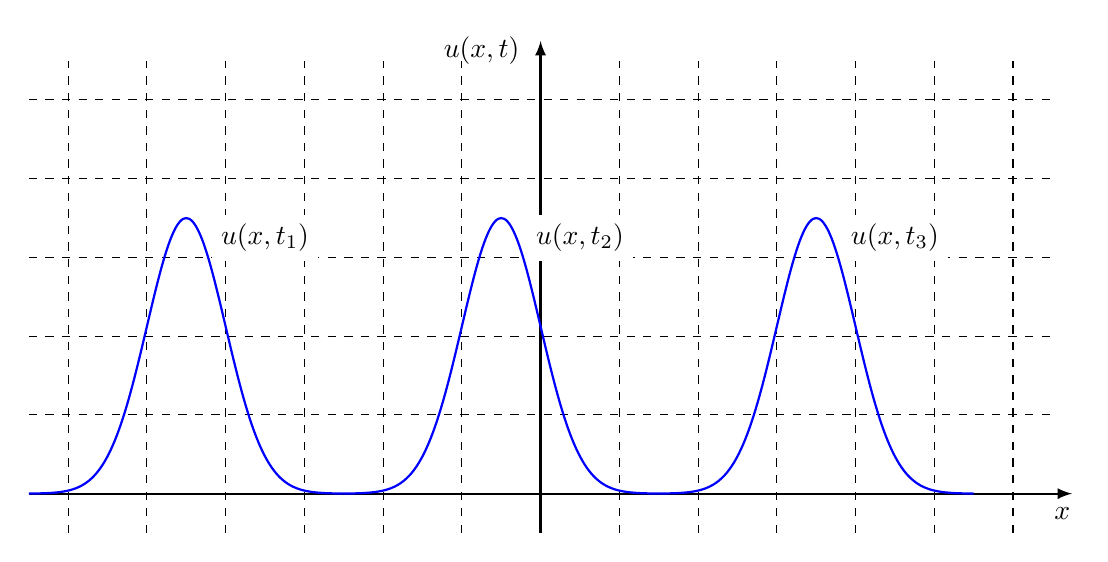
\begin{tikzpicture}
  \draw[-latex,thick] (-6.5,0) -- (6.75,0);
  \node at (6.625,-0.25) {$x$};
  \draw[-latex,thick] (0,-0.5) -- (0,5.75);
  \node at (-0.75,5.625) {$u(x,t)$};
  \foreach \x in {-6,...,6}
    \draw[dashed] (\x,-0.5) -- (\x,5.5);
  \foreach \y in {0,...,5}
    \draw[dashed] (-6.5,\y) -- (6.5,\y);

  \node[fill=white] at (-3.5,3.25) {$u(x,t_1)$}; 
  \node[fill=white] at (0.5,3.25) {$u(x,t_2)$}; 
  \node[fill=white] at (4.5,3.25) {$u(x,t_3)$}; 

  \foreach \r in {-4.5,-0.5,3.5}
    \draw[thick,color=blue]  plot[smooth,domain={{\r-2}:{\r+2}},samples=101] (\x, {3.5*exp(-2*(\x - \r)*(\x - \r)) });

%  \foreach \x in {-9,...,6}
%    \draw[-latex,thick,color=blue] ({max(-6.5,\x - 0.5*cot(60))},{max(-0.5,-6.5*tan(60) - \x*tan(60))}) -- ({min(6.5,\x + 5.5*cot(60))},{min(5.5,6.5*tan(60) - \x*tan(60))});
\end{tikzpicture}
\caption{Illustration of an example solution of uniform transport at a few snapshots in time. The initial function translates along the $x$ direction with a rate given by $c$.}
\label{Fig:pde_exampleSolutionUniformTransport}
\end{center}
\end{figure}

\begin{figure}[htb!]
\begin{center}
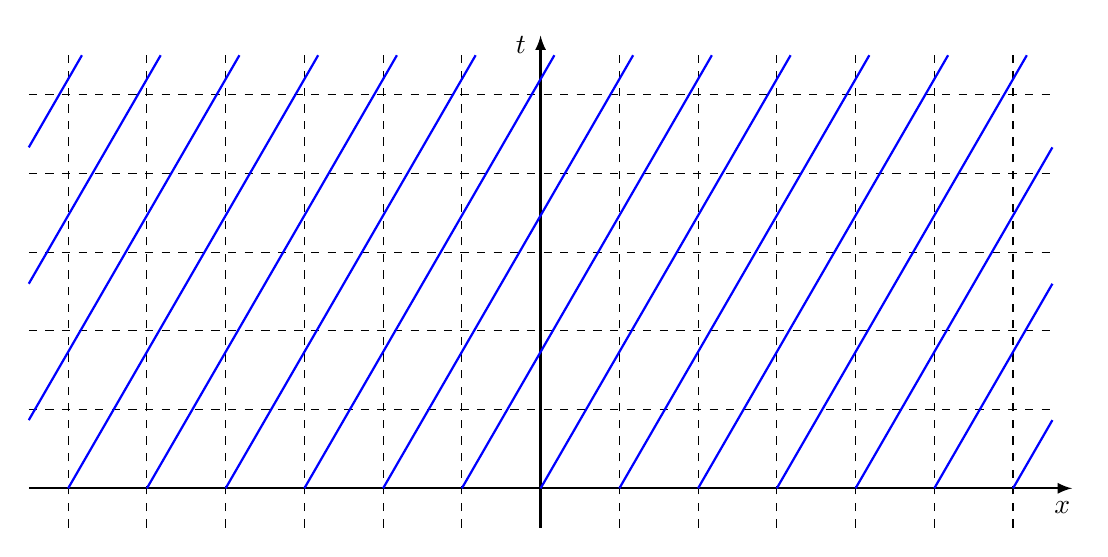
\begin{tikzpicture}
  \draw[-latex,thick] (-6.5,0) -- (6.75,0);
  \node at (6.625,-0.25) {$x$};
  \draw[-latex,thick] (0,-0.5) -- (0,5.75);
  \node at (-0.25,5.625) {$t$};
  \foreach \x in {-6,...,6}
    \draw[dashed] (\x,-0.5) -- (\x,5.5);
  \foreach \y in {0,...,5}
    \draw[dashed] (-6.5,\y) -- (6.5,\y);

  \foreach \x in {-9,...,6}
%    \draw[thick,color=blue] ({max(-6.5,\x - 0.5*cot(60))},{max(-0.5,-6.5*tan(60) - \x*tan(60))}) -- ({min(6.5,\x + 5.5*cot(60))},{min(5.5,6.5*tan(60) - \x*tan(60))});
    \draw[thick,color=blue] ({max(-6.5,\x - 0*cot(60))},{max(0,-6.5*tan(60) - \x*tan(60))}) -- ({min(6.5,\x + 5.5*cot(60))},{min(5.5,6.5*tan(60) - \x*tan(60))});
\end{tikzpicture}
\caption{Illustration of characteristic lines for the uniform transport problem.}
\label{Fig:pde_characteristicsUniformTransport}
\end{center}
\end{figure}


%%%%%%%%%%%%%%%%%%%%%%%%%%%%%%%%%%%%%%%%%%%%%%%%%%%%%%%%%%%%%%%%%%%%%%%%%%%%%%%%%%%%%%%%%%%%%%%
\subsection{Example: Transport with Absorption}

We can solve a slightly more difficult version of the same problem by including an absorption term on the right-hand side with constant absorption coefficient $\lambda$ and initial condition $u(x,0) = f(x)$:
\begin{align}
  \dho{u}{t} + c \dho{u}{x} = -\lambda u(x,t), \quad u(x,0) = f(x).
\end{align}
 The system of ordinary differential equations from method of characteristics for this problem is
\begin{subequations}
\begin{align}
  &\frac{dx}{ds} = c, \\
  &\frac{dt}{ds} = 1, \\
  &\frac{du}{ds} = -\lambda u .
\end{align}
\end{subequations}
with the initial conditions
\begin{subequations}
\begin{align}
  &x(0) = \alpha, \\
  &t(0) = 0, \\
  &u(0) = f(\alpha) .
\end{align}
\end{subequations}
The solution for the $x$ and $t$ are identical to before
\begin{subequations}
\begin{align}
  x &= c s + \alpha, \\
  t &= s.
\end{align}
The equation for $u$ is separable and leads to an exponential with a constant
\begin{align}
  u = k e^{-\lambda s} = k e^{-\lambda t} . \nonumber
\end{align}
Inserting the initial condition at $t = 0$ gives the solution for the constant
\begin{align}
  f(\alpha) =  k e^{-\lambda (0)} = k . \nonumber
\end{align}
Therefore,
\begin{align}
  u(x,t) = f(x - c t) e^{-\lambda t } .
\end{align}
\end{subequations}

\begin{figure}[tb!]
\begin{center}
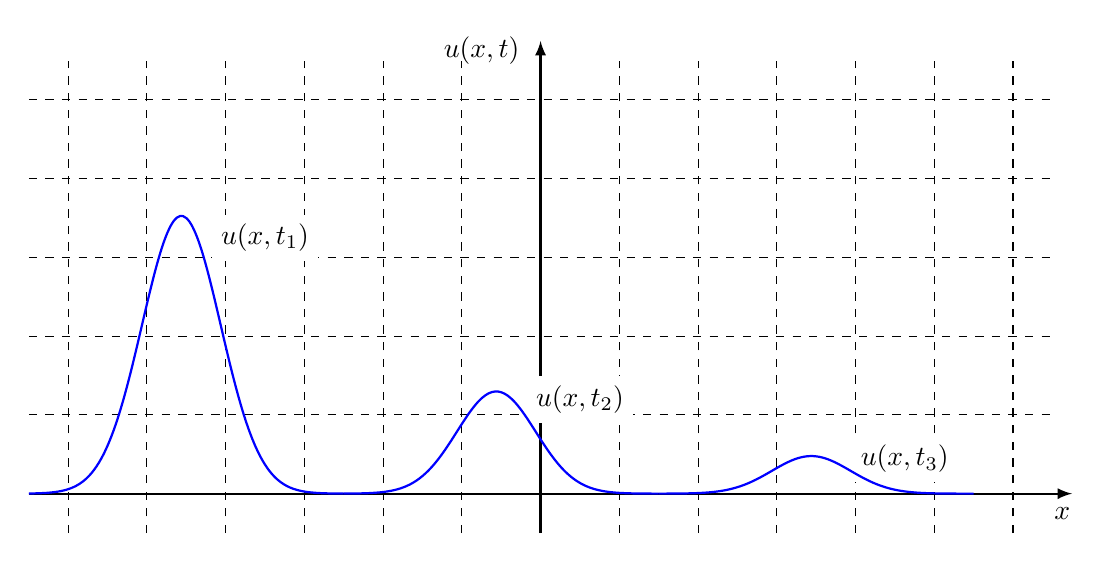
\begin{tikzpicture}
  \draw[-latex,thick] (-6.5,0) -- (6.75,0);
  \node at (6.625,-0.25) {$x$};
  \draw[-latex,thick] (0,-0.5) -- (0,5.75);
  \node at (-0.75,5.625) {$u(x,t)$};
  \foreach \x in {-6,...,6}
    \draw[dashed] (\x,-0.5) -- (\x,5.5);
  \foreach \y in {0,...,5}
    \draw[dashed] (-6.5,\y) -- (6.5,\y);

  \node[fill=white] at (-3.5,3.25) {$u(x,t_1)$}; 
  \node[fill=white] at (0.5,{3.25*exp(-1)}) {$u(x,t_2)$}; 
  \node[fill=white] at (4.625,{3.25*exp(-2)}) {$u(x,t_3)$}; 

  \foreach \r in {-4.5,-0.5,3.5}
    \draw[thick,color=blue]  plot[smooth,domain={{\r-2}:{\r+2}},samples=101] (\x, {3.5*exp(-2*(\x - \r)*(\x - \r))*exp(-0.25*(\x + 4.5)) });

%  \foreach \x in {-9,...,6}
%    \draw[-latex,thick,color=blue] ({max(-6.5,\x - 0.5*cot(60))},{max(-0.5,-6.5*tan(60) - \x*tan(60))}) -- ({min(6.5,\x + 5.5*cot(60))},{min(5.5,6.5*tan(60) - \x*tan(60))});
\end{tikzpicture}
\caption{Illustration of an example solution of transport with absorption at a few snapshots in time. The initial function translates along the $x$ direction with a rate given by $c$ and the magnitude of the function decreases with increasing time.}
\label{Fig:pde_exampleSolutionTransportWithAbsroption}
\end{center}
\end{figure}

The solution is very similar to what we had in the uniform transport case, except we how have an exponential decay term. This describes the translation of the initial condition with a speed $c$ that decreases in magnitude exponentially. This is depicted in Fig.~\ref{Fig:pde_exampleSolutionTransportWithAbsroption}. This mathematical model is used to describe moving radioactive particles or how a pulse of radiation propagates through matter.


%%%%%%%%%%%%%%%%%%%%%%%%%%%%%%%%%%%%%%%%%%%%%%%%%%%%%%%%%%%%%%%%%%%%%%%%%%%%%%%%%%%%%%%%%%%%%%%
\subsection{Example: Photon Emission from a Moving Point Source}

We have some flexibility when it comes to the initial condition. Suppose now we have a radioactive object that begins at $x = 0$ and moves with a constant speed $v$ in the positive $x$ direction that emits photons that move in the positive $x$ direction with the speed of light $c$ (we assume $v < c$). The photons are absorbed with a coefficient $\lambda$. The mathematical description of this problem is the same as what we had before, except that the initial condition is different. The mathematical model becomes
\begin{align}
  \dho{u}{t} + c \dho{u}{x} = -\lambda u(x,t), \quad u(vt,t) = u_0, \quad t \ge 0
\end{align}
The ordinary differential equations are identical, 
\begin{subequations}
\begin{align}
  &\frac{dx}{ds} = c, \\
  &\frac{dt}{ds} = 1, \\
  &\frac{du}{ds} = -\lambda u .
\end{align}
\end{subequations}
but we now have
\begin{subequations}
\begin{align}
  &x(0) = v \alpha, \\
  &t(0) = \alpha, \\
  &u(0) = u_0,
\end{align}
\end{subequations}
for the initial conditions. Solving these equations gives
\begin{subequations}
\begin{align}
  x &= c s + v \alpha, \\
  t &= s + \alpha, \\
  u &= u_0 e^{-\lambda s } .
\end{align}
\end{subequations}
The difference now being that the time coordinate $t$ is a function of $\alpha$. Eliminating $s$ from the equation for $t$ and then using the equation for $x$ to solve for $\alpha$ gives
\begin{align}
  \alpha = \frac{ ct - x }{ c - v } .
\end{align}
Plugging in $s = t - \alpha$ into the equation for $u$ gives the solution
\begin{align}
  u(x,t) = u_0 \exp \left[ -\lambda \left( t - \frac{ c t - x }{ c - v } \right) \right] , \quad vt \le x \le ct
\end{align}
To show the range solution where is valid based we study the characteristics and lines of photon emission in the $x$-$t$ plane. These are shown in Fig.~\ref{Fig:pde_photonTrajectories}. Since $t \ge 0$ and the source starts at $x = 0$, we can assert that the position coordinate in the $x$-$t$ plane cannot exceed $ct$, as it would require a particle to be emitted before $t = 0$. Likewise, the position coordinate cannot be less that $vt$ since that denotes the point photons are emitted (remember we required that they travel in the positive $x$ direction.

\begin{figure}[tb!]
\begin{center}
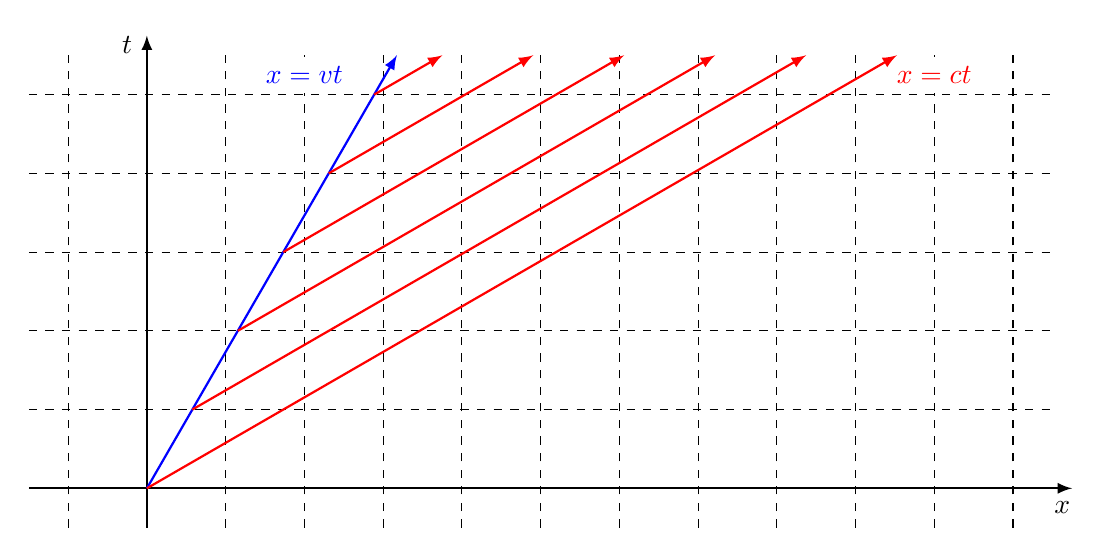
\begin{tikzpicture}
  \draw[-latex,thick] (-1.5,0) -- (11.75,0);
  \node at (11.625,-0.25) {$x$};
  \draw[-latex,thick] (0,-0.5) -- (0,5.75);
  \node at (-0.25,5.625) {$t$};
  \foreach \x in {-1,...,11}
    \draw[dashed] (\x,-0.5) -- (\x,5.5);
  \foreach \y in {0,...,5}
    \draw[dashed] (-1.5,\y) -- (11.5,\y);

  \node[color=blue, fill=white] at (2,5.25) {$x = vt$};
  \node[color=red, fill=white] at (10,5.25) {$x = ct$};
 
  \draw[-latex,thick,color=blue] (0,0) -- ({5.5*cot(60)},5.5);
  
  \foreach \t in {0,...,5}
    \draw[-latex,thick,color=red] ({\t*cot(60)},{\t})  -- ({\t*cot(60) + (5.5 - \t)*cot(30)},5.5);

%  \foreach \x in {-9,...,6}
%    \draw[-latex,thick,color=blue] ({max(-6.5,\x - 0.5*cot(60))},{max(-0.5,-6.5*tan(60) - \x*tan(60))}) -- ({min(6.5,\x + 5.5*cot(60))},{min(5.5,6.5*tan(60) - \x*tan(60))});
\end{tikzpicture}
\caption{Illustration of photon emission problem. The radioactive source travel along the blue line and the photons travel along the red lines.}
\label{Fig:pde_photonTrajectories}
\end{center}
\end{figure}

%%%%%%%%%%%%%%%%%%%%%%%%%%%%%%%%%%%%%%%%%%%%%%%%%%%%%%%%%%%%%%%%%%%%%%%%%%%%%%%%%%%%%%%%%%%%%%%
%%%%%%%%%%%%%%%%%%%%%%%%%%%%%%%%%%%%%%%%%%%%%%%%%%%%%%%%%%%%%%%%%%%%%%%%%%%%%%%%%%%%%%%%%%%%%%%
\section{First-Order Quasi-Linear PDEs}

A particular class of first-order partial differential equations that is particularly relevant to inertial confinement fusion is the quasi-linear case. These can be used to describe the flow of inviscid fluids and permit the formation of shockwaves. The first-order quasi-linear partial differential equation has the form
\begin{align}
  a(x,y,u) \dho{u}{x} + b(x,y,u) \dho{u}{y} = q(x,y,u) .
\end{align}
This differs from the linear case in that the coefficients $a$ and $b$ can now depend upon the function $u(x,t)$. The distinction between a quasi-linear and a fully nonlinear partial differential equation is that we do not allow the coefficients to depend upon the partial derivatives. Quasi-linear first-order partial differential equations, like their simpler linear kin, can be solved using the method of characteristics. In this section, we will focus explicitly on an equation called Burger's equation, which describes the flow of an inviscid fluid in one dimension with a unit speed and no external forces.

%%%%%%%%%%%%%%%%%%%%%%%%%%%%%%%%%%%%%%%%%%%%%%%%%%%%%%%%%%%%%%%%%%%%%%%%%%%%%%%%%%%%%%%%%%%%%%%
\subsection{Burger's Equation}

Burger's equation has the form
\begin{align}
  \dho{u}{t} + \frac{1}{2} \dho{}{x} ( u^2 ) = 0 , \quad u(x,0) = f(x).
\end{align}
While at first glance, this appears nonlinear, the partial derivative in $x$ can be expanded to obtain
\begin{align}
  \dho{u}{t} + u(x,t) \dho{u}{x}  = 0 , \quad u(x,0) = f(x).
\end{align}
In the form of quasi-linear partial differential equations (where we let $y = t$), the coefficients are
\begin{subequations}
\begin{align}
  a &= u, \\
  b &= 1, \\
  q &= 0.
\end{align}
\end{subequations}
Burger's equation describes a system where the speed that the function travels in the $x$ direction is equal to the magnitude of the function itself. This allows for parts of the function that are higher to ``catch up'' or ``run away'' from other parts of the solution.

Applying the method of characteristics we obtain the following system of ordinary differential equations:
\begin{subequations}
\begin{align}
  &\frac{dx}{ds} = u, \\
  &\frac{dt}{ds} = 1, \\
  &\frac{du}{ds} = 0,
\end{align}
\end{subequations}
which have the initial conditions
\begin{subequations}
\begin{align}
  &x(0) = \alpha, \\
  &t(0) = 0, \\
  &u(0) = f(\alpha) .
\end{align}
\end{subequations}
Solving for $t$ and applying the initial condition gives
\begin{subequations}
\begin{align}
  t = s .
\end{align}
Solving for $u$ yields a constant value. After applying the initial condition we get
\begin{align}
  u = f(\alpha) .
\end{align}
Finally, solving for $x$ gives
\begin{align}
  x = f(\alpha) s + \alpha = f(\alpha) t + \alpha .
\end{align}
\end{subequations}
Solving for $\alpha$ gives
\begin{align}
  \alpha = x - f(\alpha) t = x - u t .
\end{align}
Therefore, the solution becomes the implicit function
\begin{align}
  u(x,t) = f(x - u t ) .
\end{align}

This solution can lead to some interesting issues. To illustrate, let us consider the example where the initial condition is given by the following piecewise ramp function
\begin{align}
  f(x) = \left\{ \begin{array}{r l} 
  1, & \quad x < 0 \\
  1 - x, & \quad 0 \le x < 1 \\
  0, & \quad x \ge 1 \\ \end{array} \right. . 
\end{align}
Using this initial condition, we can construct a set of characteristic lines in the $x$-$t$ plane. If we parameterize the lines based on $\alpha$ we may use $x = f(\alpha) t + \alpha$ and insert the argument from the initial condition for $f(\alpha)$ replacing $x$ with $\alpha$. This gives the following functional form for the characteristics:
\begin{align}
  x(t) = \left\{ \begin{array}{r l} 
  t + \alpha, & \quad \alpha < 0 \\
  (1 - \alpha) t + \alpha, & \quad 0 \le \alpha < 1 \\
  \alpha, & \quad \alpha \ge 1 \\ \end{array} \right. . 
\end{align}

\begin{figure}[tb!]
\begin{center}
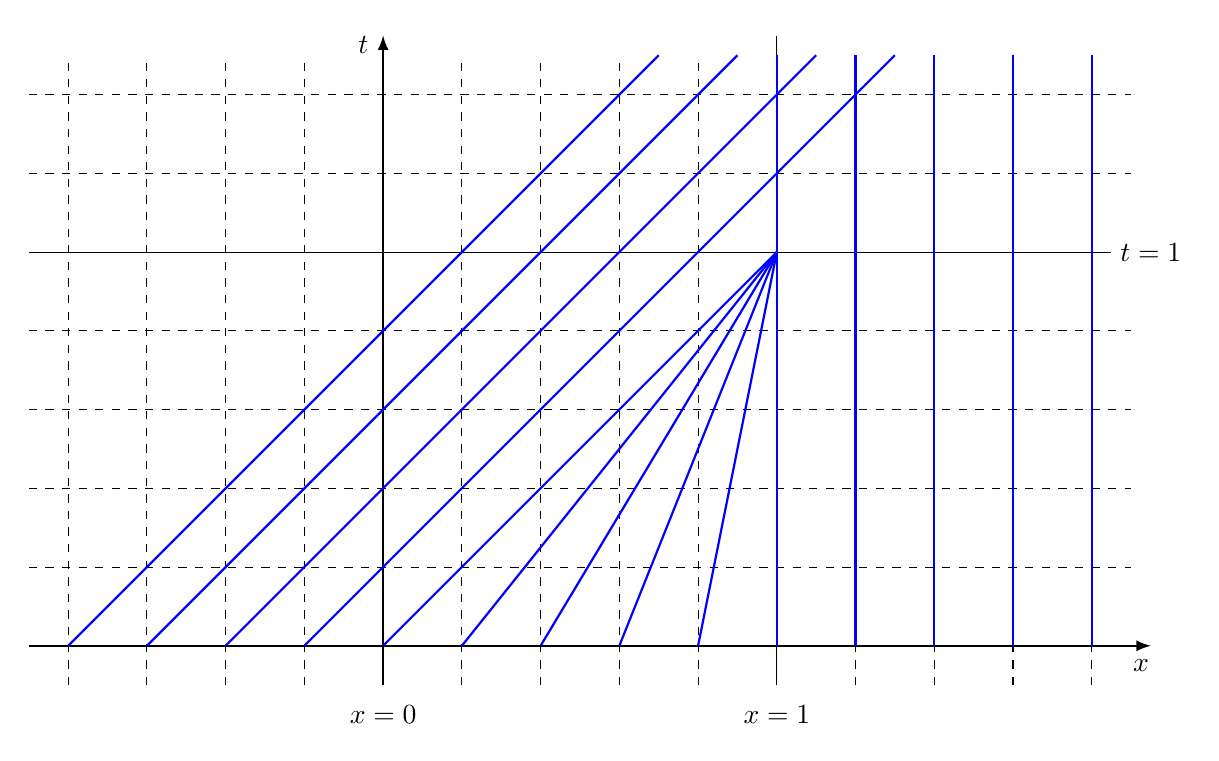
\begin{tikzpicture}
  \draw[-latex,thick] (-4.5,0) -- (9.75,0);
  \node at (9.625,-0.25) {$x$};
  \draw[-latex,thick] (0,-0.5) -- (0,7.75);
  \node at (-0.25,7.625) {$t$};
  \node at (0,-0.875) {$x = 0$};
  
  \foreach \x in {-4,...,9}
    \draw[dashed] (\x,-0.5) -- (\x,7.5);
  \foreach \y in {0,...,7}
    \draw[dashed] (-4.5,\y) -- (9.5,\y);
  \draw (5,-0.5) -- (5,7.75);
  \node at (5,-0.875) {$x = 1$};
  \draw (-4.5,5) -- (9.5,5);
  \node[fill=white] at (9.75,5) {$t=1$};

  \foreach \x in {-4,...,-1}
    \draw[thick,blue] (\x,0) -- ({\x + 7.5},7.5);

  \foreach \x in {0,...,4}
    \draw[thick,blue] (\x,0) -- (5,5);

  \foreach \x in {5,...,9}
    \draw[thick,blue] (\x,0) -- (\x,7.5);
\end{tikzpicture}
\caption{Characteristics for Burger's equation with a ramp function initial condition.}
\label{Fig:pde_burgerEquationCharacteristics_RampFunction}
\end{center}
\end{figure}

The characteristic lines are plotted in Fig.~\ref{Fig:pde_burgerEquationCharacteristics_RampFunction}. In the region $0 \le \alpha < 1$, the lines exhibit a feature that the all intersect at the point $(1,1)$ indicating that the the function appears to be converging at the time $t = 1$. 

%TODO Explain that u is a constant along a characteristic curve; explain f(alpha) in way to emphasize that alpha is merely an argument or symbol in this context; more detail on the inequalities

To obtain the solutions, we note that again $u = f(x - ut)$ and that the solution is constant along the characteristic curves. We develop solutions for three different cases for each range of $\alpha$ on these characteristic curves. For the case where $\alpha < 0$, we have $f(\alpha) = 1$. Inserting this into the equation gives 
\begin{align}
  u(x,t) = f(1) = 1, \quad \alpha < 0, \nonumber
\end{align}
or a constant solution. Putting this in terms of $x$ and $t$, this corresponds to the range where
\begin{align}
  0 > \alpha = x - f(\alpha) t = x - t \nonumber
\end{align}
or
\begin{align}
  x < t. \nonumber
\end{align}
Similarly, for the next range we have
\begin{align}
  f(x - ut) = 1 - (x - ut) = u, \quad 0 \le \alpha < 1 . \nonumber
\end{align}
Solving for $u$ gives
\begin{align}
  u = \frac{ 1 - x }{ 1 - t } . \nonumber
\end{align}
The range is found by 
\begin{align}
  0 \le \alpha = x - f(\alpha) t = x - ( 1 - \alpha ) t < 1. \nonumber
\end{align}  
Solving for $\alpha$ gives
\begin{align}
  \alpha = \frac{ x - t }{ 1 - t } . \nonumber
\end{align}
For the left side of the range where $\alpha \ge 0$,
\begin{align}
  \frac{ x - t }{ 1 - t }  \ge 0, \nonumber
\end{align}
which gives 
\begin{align}
  x \ge t. \nonumber
\end{align}
For the right side of the range where $\alpha < 1$,
\begin{align}
  \frac{ x - t }{ 1 - t }  < 1, \nonumber
\end{align}
we get 
\begin{align}
  x < 1. \nonumber
\end{align}  
Finally,
\begin{align}
  f(x - ut) = 0 = u, \quad \alpha > 1. \nonumber
\end{align}
This corresponds to the range $x \ge 1$.

%\begin{subequations}
%\begin{align}
%  u(x,t) = f(1) 
%\end{align}
%\end{subequations}

Pulling this altogether, the solution of Burger's equation is
\begin{align}
  u(x,t) = \left\{ \begin{array}{r l} 
  1, & \quad x < t \\
  \dfrac{1 - x}{1 - t}, & \quad t \le x < 1 \vspace{0.2em} \\
  0, & \quad x \ge 1 \\ \end{array} \right. . 
\end{align}
The function $u(x,t)$ is well defined until we reach the convergence point of the characteristics at $t = 1$. At this point, the solution approaches a problem point where the slope goes towards infinity and the function becomes discontinuous. Strictly speaking, a discontinuous function cannot satisfy a differential equation. Instead we will demand the differential equation be satisfied under some integral. This leads to a concept called a weak formulation, which will not be discussed here. What we need to fully define the solution, is to obtain the behavior for $t \ge 1$. To do this, we will need to derive a jump condition.

%%%%%%%%%%%%%%%%%%%%%%%%%%%%%%%%%%%%%%%%%%%%%%%%%%%%%%%%%%%%%%%%%%%%%%%%%%%%%%%%%%%%%%%%%%%%%%%
\subsection{Jump Condition for Shocks}

Before proceeding, we need to first define the notion of a conservation law. Differential equations are usually used to describe some physical process. In this case, Burger's equation is often used to describe the motion of inviscid fluids, and we can think of the conserved quantity as the amount of mass or momentum in some volume. Let us define the conservation law as the integral of $u(x,t)$ over some range $x_1$ to $x_2$:
\begin{align}
  m = \int_{x_1}^{x_2} u(x,t) dx .
\end{align}
Here $m$ denotes some conserved quantity. If we take the time rate of change of $m$, we can relate it to the difference between the inflow and outflow rates across $x_1$ and $x_2$ respectively. This gives
\begin{align}
  \frac{d}{dt} \int_{x_1}^{x_2} u(x,t) dx = \phi(u(x_1,t)) - \phi(u(x_2,t)).
\end{align}
Here $\phi(u)$ represents the flow rate of the conserved quantity across the boundary. Now, if we divide both sides by $h = x_2 - x_1$ we get
\begin{align}
  \frac{1}{x_2 - x_1} \frac{d}{dt} \int_{x_1}^{x_2} u(x,t) dx = \frac{ \phi(u(x_1,t)) - \phi(u(x_2,t)) }{ x_2 - x_1 }.
\end{align}
Next, if we take the limit is the interval $x_2 - x_1 \rightarrow 0$. The right-hand side is simply the definition of the partial derivative. We can see this if we rewrite the range to be centered around some fixed midpoint value we call $x$:
\begin{subequations}
\begin{align}
  x_1 &= x - \frac{h}{2}, \\
  x_2 &= x + \frac{h}{2}.
\end{align}
\end{subequations}
The right-hand side becomes
\begin{align}
  \dho{u}{x} = \lim_{h \rightarrow 0 } \frac{ \phi(u(x + h/2,t)) - \phi(u(x - h/2,t)) }{ h }.
\end{align}
The left-hand side becomes
\begin{align}
 \frac{d}{dt} \left(  \lim_{h \rightarrow 0 }  \frac{1}{h}  \int_{x - h/2}^{x + h/2} u(x,t) dx \right).
\end{align}
When taking the limit as $h \rightarrow 0$, we have the case where the integral goes to zero and the denominator $h$ also goes to zero. To take this limit, we employ L'Hopital's rule.
\begin{align}
  \lim_{h \rightarrow 0 } \frac{f(h)}{g(h)} = \frac{ f'(h) }{ g'(h) } .
\end{align}
To perform the derivative of the integral with respect to $h$, we note that the limits of integration depend upon $h$. This requires the use of the Leibniz rule:
\begin{align}
  \frac{d}{dt} \int_{a(t)}^{b(t)} u(x,t) dx = u(b(t),t) \frac{db}{dt} - u(a(t),t) \frac{da}{dt} + \int_{a(t)}^{b(t)} \dho{u}{t} dx .
\end{align}
The derivative becomes:
\begin{align}
  \frac{d}{dh} \left( \int_{x - h/2}^{x + h/2} u(x,t) dx \right) &=  u( x + h/2, t) \left( \frac{1}{2} \right) - u( x - h/2, t) \left( -\frac{1}{2} \right) \nonumber \\
  &= \frac{1}{2} \left[ u( x + h/2, t) + u( x - h/2, t ) \right] .
\end{align}
The last partial derivative with respect to $h$ vanishes because $u$ does not depend upon $h$. The derivative of $h$ with respect to $h$ is simply 1. So taking the limit gives
\begin{align}
  \frac{d}{dt} \left[ \frac{1}{2} \left( u(x,t) + u(x,t) \right) \right] = \frac{d}{dt} u(x,t) = \dho{u}{t} .
\end{align}
The derivative becomes the partial derivative since we are taking it with respect to some fixed value of $x$. Putting this together get a partial differential equation:
\begin{align}
  \dho{u}{t} = -\dho{}{x}( \phi(u) ) .
\end{align}
If we define
\begin{align}
  \phi(u) = \frac{1}{2} u^2(x,t)
\end{align}
we arrive at Burger's equation where $\phi(u)$ represents the outflow rate of a physical quantity.

Now let us return to our original conservation equation. Suppose we have $x_1 < x_s(t) < x_2$ where $x_s(t)$ is the time-dependent location of a shock where, based on our solution to Burger's equation, we define
\begin{align}
  u(x,t) = \left\{ \begin{array}{r l}
  u^-(x,t) & \quad x < x_s(t) \\
  u^+(x,t) & \quad x > x_s(t) \\ \end{array} \right.
\end{align}
We can write the integral term as the sum of two sub-integrals on each side of the shock
\begin{align}
  \frac{d}{dt} \left(  \int_{x_1}^{x_s(t)} u^-(x,t) dx + \int_{x_s(t)}^{x_2} u^+(x,t) dx   \right) = \phi(u^-(x_1,t)) - \phi(u^+(x_2,t)).
\end{align}
Now, to evaluate the total derivative with respect to an integral, where the limits of integration are again functions of the variable being differentiated, so we use the Leibniz rule. Taking the derivative gives
\begin{align}
  &u^-(x_s(t),t) \frac{dx_s}{dt} - u^-(x_1,t) \frac{dx_1}{dt} + \int_{x_1}^{x_s(t)} \dho{u^-}{t} dx  \nonumber \\
  &+ u^+(x_2,t) \frac{dx_2}{dt} - u^+(x_s(t),t) \frac{dx_s}{dt} + \int_{x_s(t)}^{x_2} \dho{u^+}{t} dx   \nonumber \\
  &= \phi(u^-(x_1,t)) - \phi(u^+(x_2,t)).
\end{align}
Note that $x_1$ and $x_2$ are fixed in time, so those two terms can cancel, leaving:
\begin{align}
  &u^-(x_s(t),t) \frac{dx_s}{dt} - u^+(x_s(t),t) \frac{dx_s}{dt}   \nonumber \\
  &+ \int_{x_1}^{x_s(t)} \dho{u^-}{t} dx + \int_{x_s(t)}^{x_2} \dho{u^+}{t} dx = \phi(u^-(x_1,t)) - \phi(u^+(x_2,t)).
\end{align}
Now we take the one-sided limits as $x_1 \rightarrow x_s(t)^-$ and $x_2 \rightarrow x_s(t)^+$. This causes the integral terms to vanish, leaving us with a solution we can solve for the time derivative of $x_s(t)$. This gives the \emph{Rankine-Hugoniot jump condition}:
\begin{align}
  \frac{dx_s}{dt} = \frac{ \phi(u^-(x_s(t),t)) - \phi(u^+(x_s(t),t)) }{ u^-(x_s(t),t) - u^+(x_s(t),t) } .
\end{align}
The Jump condition relates the speed of the shock to what occurs on each side of the shock.

Applying this to Burger's equation where $\phi(u) = u^2/2$, we get the jump condition is
\begin{align}
  \frac{dx_s}{dt} = \frac{1}{2} \frac{ (u^-(x_s,t))^2 - (u^+(x_s,t))^2 }{ u^-(x_s,t) - u^+(x_s,t) } .
\end{align}
Based on our solution, we have the limiting case for the left side of the shock gives $u^- = 1$ and the limiting case on the right side is $u^+ = 0$. Plugging in these values gives
\begin{align}
  \frac{dx}{dt} = \frac{1}{2} .
\end{align}
Based on the characteristics, the problem point occurs at $(1,1)$, which gives us an ``initial condition'' for the jump condition. Integrating and applying the initial condition gives
\begin{align}
  x(t) = \frac{ t + 1 }{ 2 }.
\end{align}
Therefore, the solution for the problem for $t \ge 1$ is
\begin{align}
  u(x,t) = \left\{ \begin{array}{r l}
  1, & \quad  x < \dfrac{t + 1}{2} \vspace{0.2cm} \\
  0, & \quad  x > \dfrac{t + 1}{2} \\ \end{array} \right. ,
\end{align}
with the solution we obtained previously,
\begin{align}
  u(x,t) = \left\{ \begin{array}{r l} 
  1, & \quad x < t \\
  \dfrac{1 - x}{1 - t}, & \quad t \le x < 1 \vspace{0.2em} \\
  0, & \quad x \ge 1 \\ \end{array} \right. , \nonumber
\end{align}
valid for $t < 1$. This solution is such that for $0 < t < 1$, the solution moves toward forming a shock, which occurs at $t = 1$. The shock then propagates to the right at a speed of $1/2$. This solution is shown in Fig.~\ref{Fig:pde_SolutionBurgersEquation_RampInitialCondition}. We must also incorporate this into our characteristics. A revised plot for the characteristics that includes the jump condition is given in Fig.~\ref{Fig:pde_burgerEquationCharacteristics_RampFunction_Revised}.


\begin{figure}[htb!]
\begin{center}
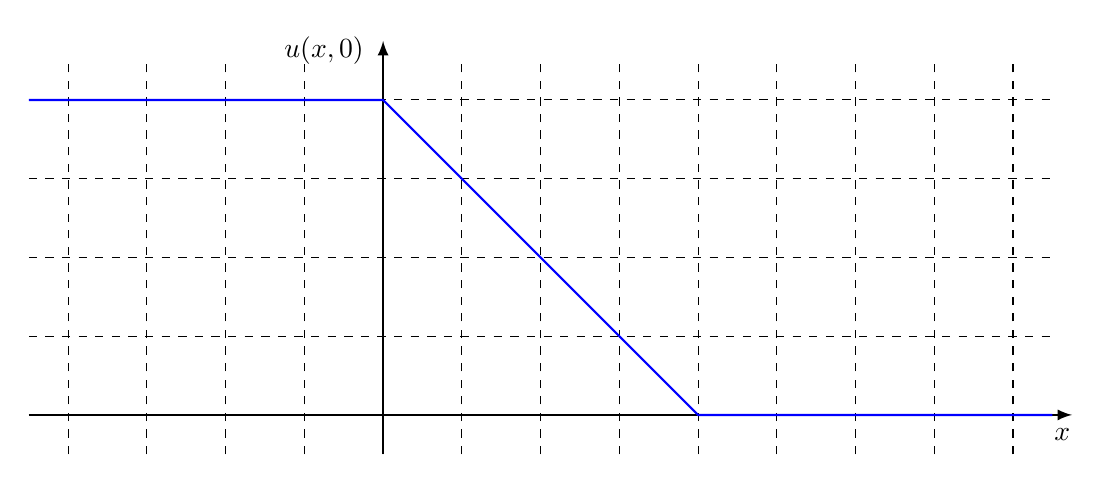
\begin{tikzpicture}
  \draw[-latex,thick] (-4.5,0) -- (8.75,0);
  \node at (8.625,-0.25) {$x$};
  \draw[-latex,thick] (0,-0.5) -- (0,4.75);
  \node at (-0.75,4.625) {$u(x,0)$};
  \foreach \x in {-4,...,8}
    \draw[dashed] (\x,-0.5) -- (\x,4.5);
  \foreach \y in {0,...,4}
    \draw[dashed] (-4.5,\y) -- (8.5,\y);

  \draw[thick,color=blue]  (-4.5,4) -- (0,4) -- (4,0) -- (8.5,0);
\end{tikzpicture}
%%%%%
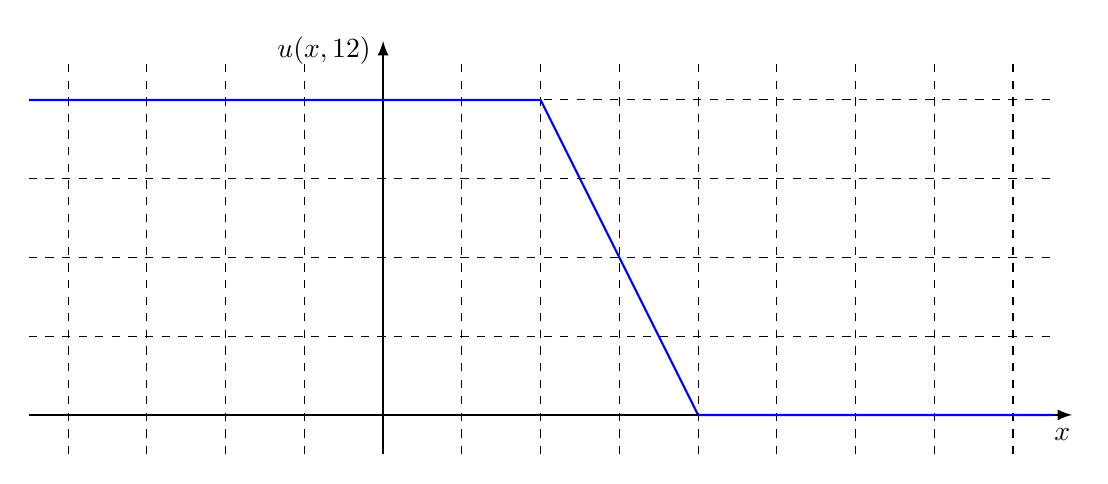
\begin{tikzpicture}
  \draw[-latex,thick] (-4.5,0) -- (8.75,0);
  \node at (8.625,-0.25) {$x$};
  \draw[-latex,thick] (0,-0.5) -- (0,4.75);
  \node at (-0.75,4.625) {$u(x,\rfrac{1}{2})$};
  \foreach \x in {-4,...,8}
    \draw[dashed] (\x,-0.5) -- (\x,4.5);
  \foreach \y in {0,...,4}
    \draw[dashed] (-4.5,\y) -- (8.5,\y);

  \draw[thick,color=blue]  (-4.5,4) -- (2,4) -- (4,0) -- (8.5,0);
\end{tikzpicture}
%%%%%
\begin{tikzpicture}
  \draw[-latex,thick] (-4.5,0) -- (8.75,0);
  \node at (8.625,-0.25) {$x$};
  \draw[-latex,thick] (0,-0.5) -- (0,4.75);
  \node at (-0.75,4.625) {$u(x,1)$};
  \foreach \x in {-4,...,8}
    \draw[dashed] (\x,-0.5) -- (\x,4.5);
  \foreach \y in {0,...,4}
    \draw[dashed] (-4.5,\y) -- (8.5,\y);

  \draw[thick,color=blue]  (-4.5,4) -- (4,4) -- (4,0) -- (8.5,0);
\end{tikzpicture}
%%%%%
\begin{tikzpicture}
  \draw[-latex,thick] (-4.5,0) -- (8.75,0);
  \node at (8.625,-0.25) {$x$};
  \draw[-latex,thick] (0,-0.5) -- (0,4.75);
  \node at (-0.75,4.625) {$u(x,2)$};
  \foreach \x in {-4,...,8}
    \draw[dashed] (\x,-0.5) -- (\x,4.5);
  \foreach \y in {0,...,4}
    \draw[dashed] (-4.5,\y) -- (8.5,\y);

  \draw[thick,color=blue]  (-4.5,4) -- (6,4) -- (6,0) -- (8.5,0);
\end{tikzpicture}
\caption{Illustration of a solution to Burger's equation with an initial ramp function.}
\label{Fig:pde_SolutionBurgersEquation_RampInitialCondition}
\end{center}
\end{figure}
\clearpage

\begin{figure}[tb!]
\begin{center}
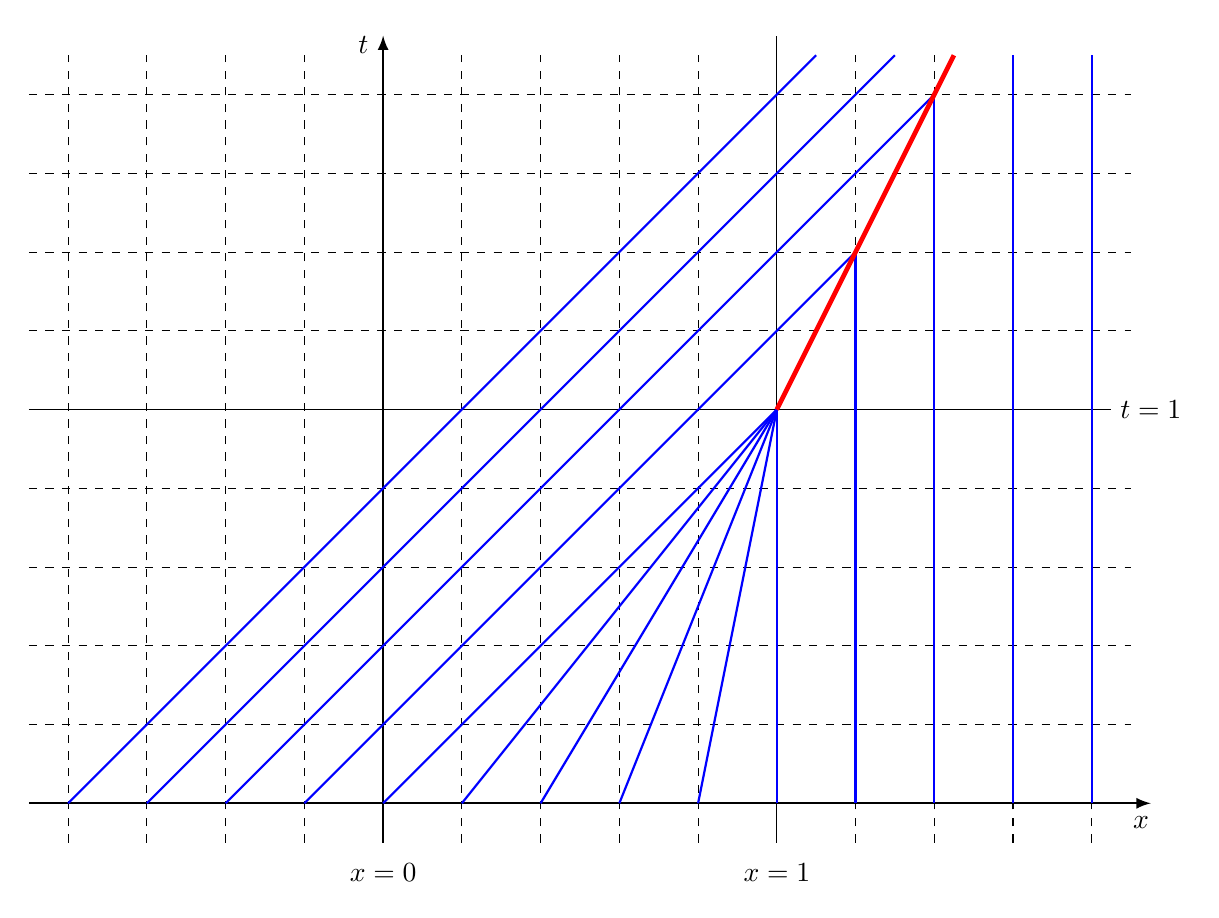
\begin{tikzpicture}
  \draw[-latex,thick] (-4.5,0) -- (9.75,0);
  \node at (9.625,-0.25) {$x$};
  \draw[-latex,thick] (0,-0.5) -- (0,9.75);
  \node at (-0.25,9.625) {$t$};
  \node at (0,-0.875) {$x = 0$};
  
  \foreach \x in {-4,...,9}
    \draw[dashed] (\x,-0.5) -- (\x,9.5);
  \foreach \y in {0,...,9}
    \draw[dashed] (-4.5,\y) -- (9.5,\y);
  \draw (5,-0.5) -- (5,9.75);
  \node at (5,-0.875) {$x = 1$};
  \draw (-4.5,5) -- (9.5,5);
  \node[fill=white] at (9.75,5) {$t=1$};

  \foreach \r in {-4,-3}
    \draw[thick,blue] (\r,0) -- ({\r + 9.5},9.5);

  \foreach \r in {-2,-1}
    \draw[thick,blue] (\r,0) -- ({5 - \r},{5 - 2*\r});
%    \draw[thick,blue] (\x,0) -- ({\x + 7.5},7.5);

  \foreach \x in {0,...,4}
    \draw[thick,blue] (\x,0) -- (5,5);

  \foreach \x in {5,...,9}
    \draw[thick,blue] (\x,0) -- (\x,{min(9.5,2*\x-5)});
    
  \draw[red,line width=0.6mm] (5,5) -- (7.25,9.5);
\end{tikzpicture}
\caption{Characteristics for Burger's equation with a ramp function initial condition including the Rankine-Hugoniot jump condition after the shock formation. The shock front is denoted by a thick red line.}
\label{Fig:pde_burgerEquationCharacteristics_RampFunction_Revised}
\end{center}
\end{figure}


%%%%%%%%%%%%%%%%%%%%%%%%%%%%%%%%%%%%%%%%%%%%%%%%%%%%%%%%%%%%%%%%%%%%%%%%%%%%%%%%%%%%%%%%%%%%%%%
\subsection{Entropy Condition and Rarefactions}

It is also possible to have cases where we have multiple valid solutions from quasi-linear partial differential equations that satisfy the jump conditions. In these cases, the mathematical model does not have sufficient information to uniquely determine the physics and we need to impose additional constraints based upon physics considerations. We illustrate this case for Burger's equation with the following initial condition:
\begin{align}
  f(x) = \left\{ \begin{array}{r l} 
  0, & \quad x < 0 \\
  1, & \quad x \ge 0 \\ \end{array} \right. . 
\end{align}
This initial condition has a discontinuity at $x = 0$. A key feature here is that initial condition is greater to the right and smaller to the left. In these cases, we may run into the issue of multiple valid solutions.

Again, the characteristic curves along $x$ parameterized by $\alpha$ are given by
\begin{align}
  x(\alpha) = f(\alpha) t + \alpha . \nonumber
\end{align}
This implies
\begin{align}
  x(\alpha) = \left\{ \begin{array}{r l}
  \alpha, & \quad \alpha < 0 \\
  t + \alpha, & \quad \alpha \ge 0 \\ \end{array} \right. .
\end{align}
These characteristic curves produce the solution
\begin{align}
  u(x,t) = \left\{ \begin{array}{r l}
  0, & \quad x < 0 \\
  ?, & \quad 0 \ge x < t \\
  1, & \quad x > t \\ \end{array} \right. .
\end{align}
Here we have characteristic curves, and therefore solutions, for the region $x < 0$ and $x > t$, but no information about $0 < x < t$. In other words, the range between $x = 0$ and the edge of the shock is undefined for $t > 0$. The differential equation alone does not provide enough information.

We must therefore devise solutions that both satisfy both the differential equation and the Rankine-Hugoniot jump conditions. A possible solution that does this is to have the shock move to the right at the speed of $1/2$ with a value of $u = 1$ ahead of the shock and $u = 0$ behind it. We call this possible solution
\begin{align}
  u(x,t) \stackrel{?}{=} u_1(x,t) = \left\{ \begin{array}{r l}
  0, & \quad x < \dfrac{t}{2} \vspace{0.2cm} \\
  1, & \quad x \ge \dfrac{t}{2} \\ \end{array} \right. .
\end{align}
Another possible solution continuously connects the points between $x = 0$ and $x = t$. We call this solution
\begin{align}
  u(x,t) \stackrel{?}{=} u_2(x,t) = \dfrac{x}{t} .
\end{align}
This also satisfies the differential equation and for $t \rightarrow 0$ limits to the initial and jump conditions. Both candidate solutions are plotting alongside the initial condition in Fig.~\ref{Fig:pde_SolutionBurgersEquation_Rarefaction_PossibleSolutions}.

Resolving which one of these two solutions most matches reality invokes the second law of thermodynamics, which states that in an isolated system the entropy increases. (Note that if we have external forces, the entropy could decrease locally so long as the net increase in entropy from generating the external force is positive.) The entropy condition whether a shock is allowed to propagate relates the shock speed to the derivative of the inflow/outflow rates:
\begin{align}
  \phi'(u^-) > \frac{dx_s}{dt} > \phi'(u^+).
\end{align}
We only admit shocks that follow this condition. If the curve is not a discontinuous shock, then we cannot apply this conditions.

\begin{figure}[tb!]
\begin{center}
\begin{tikzpicture}
  \draw[-latex,thick] (-4.5,0) -- (8.75,0);
  \node at (8.625,-0.25) {$x$};
  \draw[-latex,thick] (0,-0.5) -- (0,4.75);
  \node at (-0.75,4.625) {$u(x,0)$};
  \foreach \x in {-4,...,8}
    \draw[dashed] (\x,-0.5) -- (\x,4.5);
  \foreach \y in {0,...,4}
    \draw[dashed] (-4.5,\y) -- (8.5,\y);

  \draw[thick,color=blue]  (-4.5,0) -- (0,0) -- (0,4) -- (8.5,4);
\end{tikzpicture}
%%%%%
\begin{tikzpicture}
  \draw[-latex,thick] (-4.5,0) -- (8.75,0);
  \node at (8.625,-0.25) {$x$};
  \draw[-latex,thick] (0,-0.5) -- (0,4.75);
  \node at (-0.75,4.625) {$u_1(x,1)$};
  \foreach \x in {-4,...,8}
    \draw[dashed] (\x,-0.5) -- (\x,4.5);
  \foreach \y in {0,...,4}
    \draw[dashed] (-4.5,\y) -- (8.5,\y);

  \draw[thick,color=blue]  (-4.5,0) -- (2,0) -- (2,4) -- (8.5,4);
\end{tikzpicture}
%%%%%
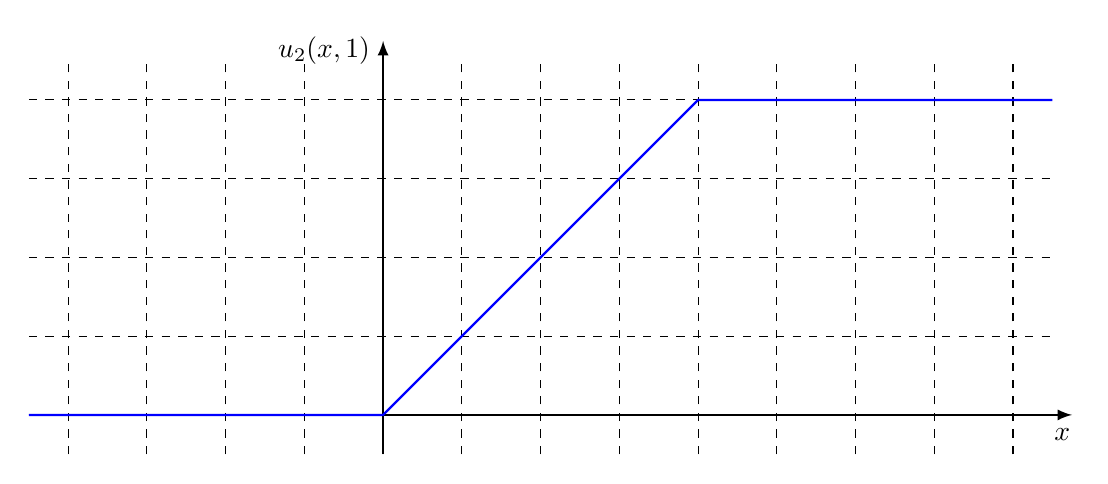
\begin{tikzpicture}
  \draw[-latex,thick] (-4.5,0) -- (8.75,0);
  \node at (8.625,-0.25) {$x$};
  \draw[-latex,thick] (0,-0.5) -- (0,4.75);
  \node at (-0.75,4.625) {$u_2(x,1)$};
  \foreach \x in {-4,...,8}
    \draw[dashed] (\x,-0.5) -- (\x,4.5);
  \foreach \y in {0,...,4}
    \draw[dashed] (-4.5,\y) -- (8.5,\y);

  \draw[thick,color=blue]  (-4.5,0) -- (0,0) -- (4,4) -- (8.5,4);
\end{tikzpicture}
\caption{Illustration of the initial condition and two possible solutions of Burger's equation at $t = 1$.}
\label{Fig:pde_SolutionBurgersEquation_Rarefaction_PossibleSolutions}
\end{center}
\end{figure}
\clearpage

\begin{figure}[tb!]
\begin{center}
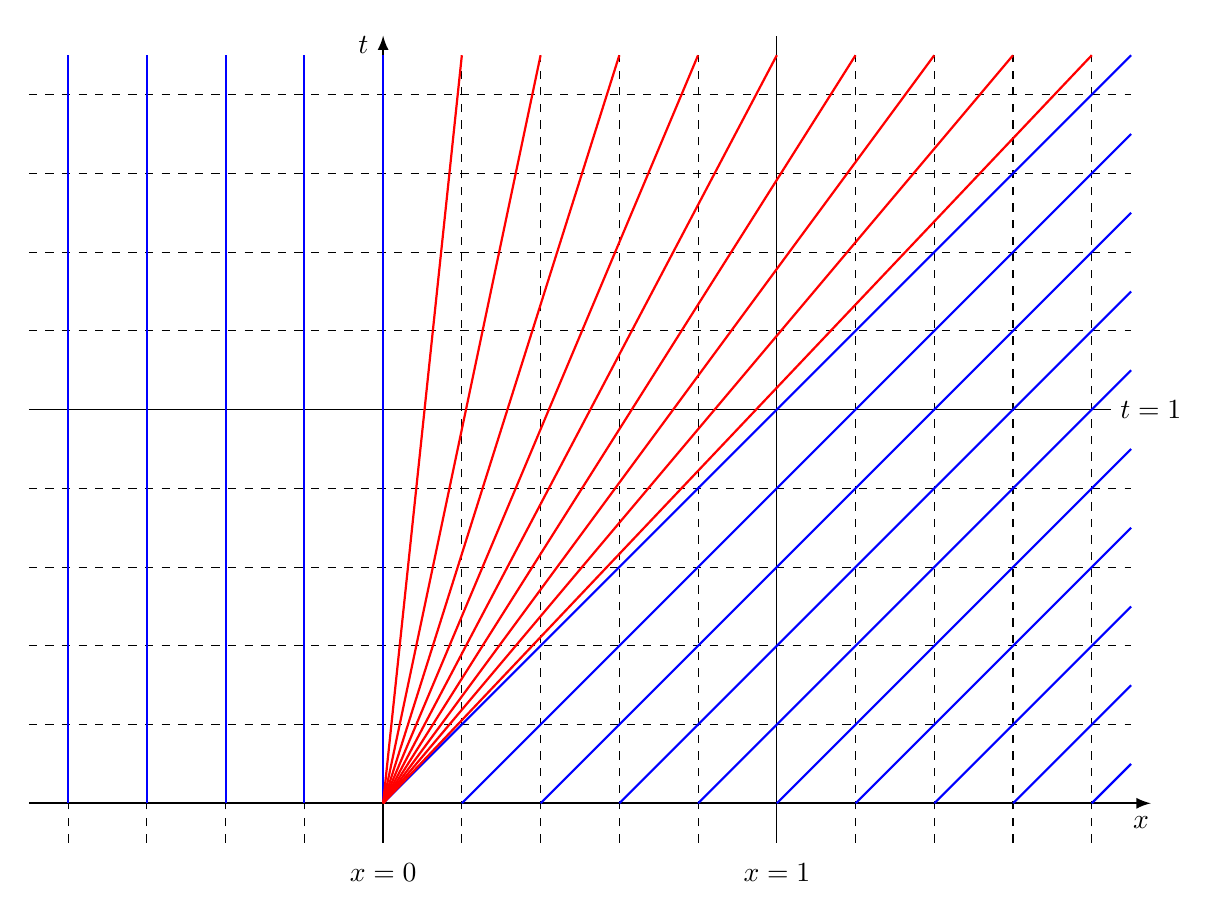
\begin{tikzpicture}
  \draw[-latex,thick] (-4.5,0) -- (9.75,0);
  \node at (9.625,-0.25) {$x$};
  \draw[-latex,thick] (0,-0.5) -- (0,9.75);
  \node at (-0.25,9.625) {$t$};
  \node at (0,-0.875) {$x = 0$};
  
  \foreach \x in {-4,...,9}
    \draw[dashed] (\x,-0.5) -- (\x,9.5);
  \foreach \y in {0,...,9}
    \draw[dashed] (-4.5,\y) -- (9.5,\y);
  \draw (5,-0.5) -- (5,9.75);
  \node at (5,-0.875) {$x = 1$};
  \draw (-4.5,5) -- (9.5,5);
  \node[fill=white] at (9.75,5) {$t=1$};

  \foreach \r in {-4,...,0}
    \draw[thick,blue] (\r,0) -- (\r,9.5);

  \foreach \r in {0,...,9}
    \draw[thick,blue] (\r,0) -- (9.5,{9.5-\r});

  \foreach \r in {1,...,9}
    \draw[thick,red] (0,0) -- (\r,9.5);

\end{tikzpicture}
\caption{Characteristics for Burger's equation a step initial condition including a rarefaction solution (red) that satisfies the entropy condition.}
\label{Fig:pde_burgerEquationCharacteristics_Rarefaction}
\end{center}
\end{figure}


For our case, the shock speed is $1/2$ and
\begin{align}
  \phi'(u) = \frac{d}{du} \left( \frac{u^2}{2} \right) = u .
\end{align}
For candidate solution 1, we have a traveling shock with $u^- = 0$, which is obviously not greater than $1/2$, and neither is $u^+ = 1$ less than $1/2$. Therefore, we can reject this solution because it does not increase entropy. Candidate solution 2 is not a shock, rather it is a continuous solution. Since we have rejected the shock, it is reasonable to accept $u_2(x,t)$. Therefore, our solution becomes
\begin{align}
  u(x,t) = \left\{ \begin{array}{r l}
  0, & \quad x < 0 \vspace{0.2cm} \\
  \dfrac{x}{t}, & \quad 0 \ge x < t \vspace{0.2cm}  \\
  1, & \quad x > t \\ \end{array} \right. .
\end{align}

The characteristic lines for the solution are plotted in Fig.~\ref{Fig:pde_burgerEquationCharacteristics_Rarefaction}. The solution $u_2 = x/t$ is called a \emph{rarefaction wave}, which means the density of the quantity decreases as the solution propagates. From the plot, we see characteristic lines spreading out in a fanlike pattern. This may be interpreted as for each point within the rarefaction for $t > 0$, we can trace the solution back in time to the point $x = 0, t = 0$.

Before concluding the discussion on shocks and rarefactions, one point to bring up that is that we have an overall conservation of area under the curve at all times. In our examples, the area is infinite so this is not apparent; however, these are contrived cases. In real-world problems, we have a finite system. As there is no absorption or growth term, we expect the total amount of the quantity to be constant, and just redistributing in space. We saw the similar case with the uniform transport problem where the quantity underwent simple translation.


%%%%%%%%%%%%%%%%%%%%%%%%%%%%%%%%%%%%%%%%%%%%%%%%%%%%%%%%%%%%%%%%%%%%%%%%%%%%%%%%%%%%%%%%%%%%%%%
%%%%%%%%%%%%%%%%%%%%%%%%%%%%%%%%%%%%%%%%%%%%%%%%%%%%%%%%%%%%%%%%%%%%%%%%%%%%%%%%%%%%%%%%%%%%%%%
\section{Heat Equation in 1-D}

The heat equation is a partial differential equation that was first proposed to study the time-dependent transfer of thermal energy. Using this equation, we are able to obtain the temperature distribution through some object given some prescribed initial condition and boundary conditions. While this may seem limited in scope, it turns out that the partial differential equations used to describe many other physical phenomena are either identical or similar in form to the heat equation. This includes mass transport through materials, neutron diffusion, and the potential functions of electromagnetism. The heat equation is sometimes (more precisely) referred to as the diffusion equation, but the former usage is more common because of its historical development.

The heat equation has the generic 3-D form
\begin{align}
  \dho{u}{t} - \alpha \nabla^2 u(\pos,t) = 0.
\end{align}
The parameter $\alpha$ is often referred to as the diffusion coefficient. The negative sign on the Laplacian has a physical interpretation related to the entropy condition we discussed for the shock problem. Specifically, the negative sign leads to an overall tendency of a physical quantity to spread out uniformly, which is consistent with the second law of thermodynamics.

In this section we will study the case of one spatial dimension. In Cartesian coordinates the 1-D heat equation has the form,
\begin{align}
  \dho{u}{t} - \alpha \dhotwo{u}{x} = 0, \quad 0 \le x \le L, \quad t \ge 0 .
\end{align}
Since we have three total derivatives: one in time and two in space, we need to specify three conditions on the solution. The first of these specifies an initial condition
\begin{align}
  u(x,0) = f(x), \quad 0 \le x \le L .
\end{align}
Here the solution is allowed to take any function at time $t = 0$. As with the ordinary differential equations, we must also specify boundary conditions at $x = 0$ and $x = L$. Options for this are the same as for second-order ordinary differential equations. The first, and simplest, are the Dirichlet boundary conditions, which specify the solution at the boundaries. The second is the Neumann boundary condition, which specifies the derivative in the direction normal to the boundary. The final condition is the Robin boundary condition, which is a combination of these two.

In cylindrical coordinates, the 1-D heat equation is obtained by expanding out the Laplacian and keeping the radial term
\begin{align}
  \dho{u}{t} - \frac{\alpha}{r} \dho{}{r} \left( r \dho{u}{r} \right) = 0, \quad 0 \le x \le R, \quad t \ge 0 .
\end{align}
In spherical coordinates the 1-D heat equation is
\begin{align}
  \dho{u}{t} - \frac{\alpha}{r^2} \dho{}{r} \left( r^2 \dho{u}{r} \right) = 0, \quad 0 \le x \le R, \quad t \ge 0 .
\end{align}

The heat equation also has a couple variants. The first adds an inhomogeneous term, which could be, for example, the generation of heat within the domain. We can also add an absorption term involving $u(x,t)$, which is common when we are studying mass or neutron diffusion where materials can be removed through chemical or nuclear reactions respectively. Finally, we can add a drift term involving the spatial partial derivative, which causes the solution to transport in time, identical to what we say when studying the first-order partial differential equations.


%%%%%%%%%%%%%%%%%%%%%%%%%%%%%%%%%%%%%%%%%%%%%%%%%%%%%%%%%%%%%%%%%%%%%%%%%%%%%%%%%%%%%%%%%%%%%%%
\subsection{Fourier Series Expansions}

Unfortunately, solutions for the heat equation do not often have a closed form, and we need to express the solution as an infinite series with a particular choice of orthogonal basis functions. Orthogonal functions satisfy the property that if you have two functions $f_n(x)$ and $f_m(x)$ on some domain, then if we take the inner product of those two functions only terms where $n = m$ are nonzero. In terms of functions, the inner product is the integral over the entire domain. This is stated as
\begin{align}
  \int_{-\infty}^\infty f_n(x) f_m(x) dx = c_n \delta_{mn} .
\end{align}
Here $c_n$ is some constant and $\delta_{mn}$ is the Kronecker delta function, which is
\begin{align}
  \delta_{mn} = \left\{ \begin{array}{r l}
  1 & \quad m = n, \\
  0 & \quad m \ne n \\ \end{array} \right. .
\end{align} 

In Cartesian coordinates, the choice of orthogonal basis function are the trigonometric functions where we define the domain to be in such a way as to include full periods of that function. Let us assume the domain $-L \le x \le L$. (This does not lose generality, as we can always do a coordinate transformation to scale and shift to obtain any domain we like.) The trigonometric functions satisfy an orthogonality property. For the case of sine functions where $n > 0$ or $m > 0$ exclusively (not both equal to zero),
\begin{subequations}
\begin{align}
  \int_{-L}^L \sin \left( \frac{m \pi x }{ L } \right) \sin \left( \frac{n \pi x }{ L } \right) dx = L \delta_{nm} .
\end{align}
Similarly the cosine functions satisfy
\begin{align}
  \int_{-L}^L \cos \left( \frac{m \pi x }{ L } \right) \cos \left( \frac{n \pi x }{ L } \right) dx = L \delta_{nm} .
\end{align}
Furthermore any product of sine and cosine functions integrated over the domain
\begin{align}
  \int_{-L}^L \sin \left( \frac{m \pi x }{ L } \right) \cos \left( \frac{n \pi x }{ L } \right) dx = 0 .
\end{align}
Note that if both $n = m = 0$ then we obviously get
\begin{align}
  \int_{-L}^L dx = 2 L .
\end{align}
\end{subequations}

The fundamental idea of the Fourier series is that any continuous function on the domain can be expressed using an infinite sum of trigonometric functions
\begin{align}
  f(x) = c_0 + \sum_{n=1}^\infty a_n \sin \left( \frac{n \pi x }{ L } \right) + \sum_{n=1}^\infty b_n \cos \left( \frac{n \pi x }{ L } \right) , \quad -L < x < L .
\end{align}
Here $a_n$ and $b_n$ are coefficients that are used to fit the specific functions. These can be found by taking integrals. First, let us integrate the function over the domain
\begin{align}
  \int_{-L}^L f(x) dx = \int_{-L}^L c_0 dx + \sum_{n=1}^\infty a_n \int_{-L}^L \sin \left( \frac{n \pi x }{ L } \right) dx + \sum_{n=1}^\infty b_n \int_{-L}^L \cos \left( \frac{n \pi x }{ L } \right) dx .
\end{align}
Because of orthogonality, all of the terms involving sines and cosines vanish leaving us with $2 L c_0$. Therefore, the coefficient is
\begin{align}
  c_0 = \frac{1}{2L} \int_{-L}^L f(x) dx .
\end{align}
The $a_n$ coefficients for $n > 0$ can be found by multiplying by the sine function with period $n$ and integrating over the domain:
\begin{align}
  \int_{-L}^L  \sin \left( \frac{n \pi x }{ L } \right) f(x) dx &= \int_{-L}^L c_0  \sin \left( \frac{n \pi x }{ L } \right) dx \nonumber \\ &+ \sum_{n=1}^\infty a_n \int_{-L}^L  \sin \left( \frac{n \pi x }{ L } \right) \sin \left( \frac{n \pi x }{ L } \right) dx \nonumber \\ &+ \sum_{n=1}^\infty b_n \int_{-L}^L  \sin \left( \frac{n \pi x }{ L } \right) \cos \left( \frac{n \pi x }{ L } \right) dx .
\end{align}
Using the orthogonality, only the $a_n$ term survives, giving
\begin{align}
  a_n = \frac{1}{L} \int_{-L}^L \sin \left( \frac{n \pi x }{ L } \right) f(x) dx , \quad n > 0.
\end{align}
The same process can be done using the cosine function. The result of this is
\begin{align}
  b_n = \frac{1}{L} \int_{-L}^L \cos \left( \frac{n \pi x }{ L } \right) f(x) dx , \quad n > 0.
\end{align}

% Discuss a finite domain

\begin{figure}[tb!]
\begin{center}
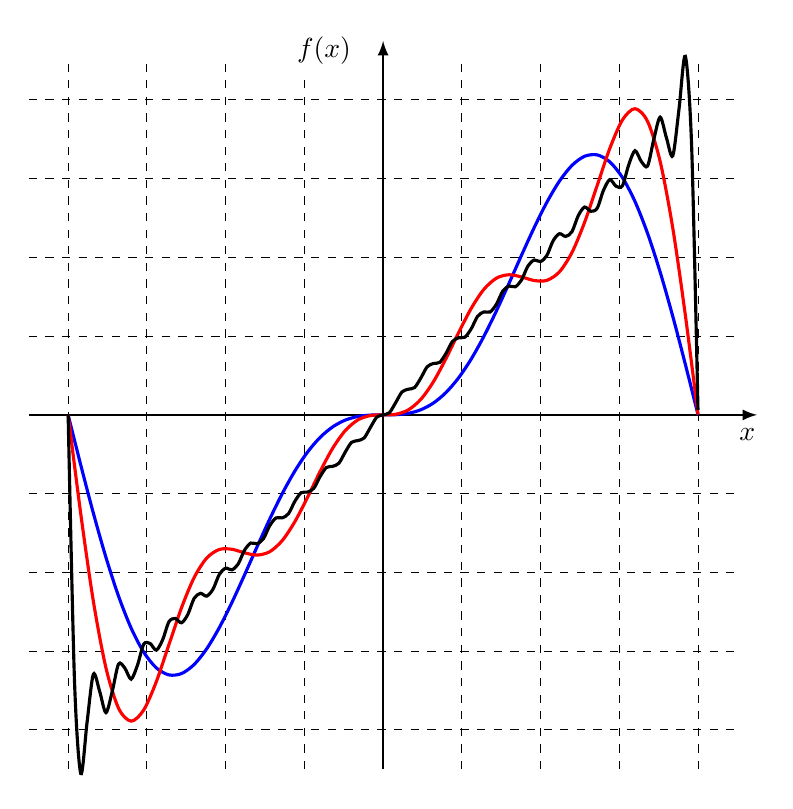
\begin{tikzpicture}
  \draw[-latex,thick] (-4.5,0) -- (4.75,0);
  \node at (4.625,-0.25) {$x$};
  \draw[-latex,thick] (0,-4.5) -- (0,4.75);
  \foreach \x in {-4,...,4}
    \draw[dashed] (\x,-4.5) -- (\x,4.5);
  \foreach \y in {-4,...,4}
    \draw[dashed] (-4.5,\y) -- (4.5,\y);

  \node[fill=white] at (-0.75,4.625) {$f(x)$};

  \draw[line width=0.4mm,color=blue]  plot[smooth,domain={-4:+4},samples=51] 
  (\x, {8/( 1*pi)*sin(deg( 1*pi*\x/4)) - 8/( 2*pi)*sin(deg( 2*pi*\x/4)) }  );

  \draw[line width=0.4mm,color=red]  plot[smooth,domain={-4:+4},samples=51] 
  (\x, {8/( 1*pi)*sin(deg( 1*pi*\x/4)) - 8/( 2*pi)*sin(deg( 2*pi*\x/4)) + 8/( 3*pi)*sin(deg( 3*pi*\x/4)) - 8/( 4*pi)*sin(deg( 4*pi*\x/4)) }  );

  \draw[line width=0.4mm,color=black]  plot[smooth,domain={-4:+4},samples=101] 
  (\x, {8/( 1*pi)*sin(deg( 1*pi*\x/4)) - 8/( 2*pi)*sin(deg( 2*pi*\x/4)) + 8/( 3*pi)*sin(deg( 3*pi*\x/4)) - 8/( 4*pi)*sin(deg( 4*pi*\x/4)) 
      + 8/( 5*pi)*sin(deg( 5*pi*\x/4)) - 8/( 6*pi)*sin(deg( 6*pi*\x/4)) + 8/( 7*pi)*sin(deg( 7*pi*\x/4)) - 8/( 8*pi)*sin(deg( 8*pi*\x/4)) 
      + 8/( 9*pi)*sin(deg( 9*pi*\x/4)) - 8/(10*pi)*sin(deg(10*pi*\x/4)) + 8/(11*pi)*sin(deg(11*pi*\x/4)) - 8/(12*pi)*sin(deg(12*pi*\x/4)) 
      + 8/(13*pi)*sin(deg(13*pi*\x/4)) - 8/(14*pi)*sin(deg(14*pi*\x/4)) + 8/(15*pi)*sin(deg(15*pi*\x/4)) - 8/(16*pi)*sin(deg(16*pi*\x/4)) 
      + 8/(17*pi)*sin(deg(17*pi*\x/4)) - 8/(18*pi)*sin(deg(18*pi*\x/4)) + 8/(19*pi)*sin(deg(19*pi*\x/4)) - 8/(20*pi)*sin(deg(20*pi*\x/4)) 
      + 8/(21*pi)*sin(deg(21*pi*\x/4)) - 8/(22*pi)*sin(deg(22*pi*\x/4)) + 8/(23*pi)*sin(deg(23*pi*\x/4)) - 8/(24*pi)*sin(deg(24*pi*\x/4)) }  );
\end{tikzpicture}
\caption{Illustration of a Fourier series expansion of $f(x) = x, -1 \le x \le 1$ for $N = 2$ terms (blue), $N = 4$ terms (red), and $N = 24$ terms (black).}
\label{Fig:pde_exampleFourierSeries_LinearFunction}
\end{center}
\end{figure}


Before proceeding to try to apply this to partial differential equation, let us do a few examples. The first case we will consider is the linear function
\begin{align}
  f(x) = \frac{x}{L} , \quad -L \le x \le L .
\end{align}
Applying the equations to estimate coefficients, we get
\begin{subequations}
\begin{align}
  c_0 &= \frac{1}{2L} \int_{-L}^L \frac{x}{L} dx = 0 , \\
  a_n &= \frac{1}{L} \int_{-L}^L \sin \left( \frac{n \pi x }{ L } \right) \frac{x}{L} dx = - \frac{2}{n\pi} \cos( n \pi ) , \quad n > 0, \\
  b_n &= \frac{1}{L} \int_{-L}^L \cos \left( \frac{n \pi x }{ L } \right) \frac{x}{L} dx = 0, \quad n > 0.
\end{align}
\end{subequations}
We note that we can write the cosine term in the $a_n$ coefficients as
\begin{align}
  \cos( n \pi ) = (-1)^n . \nonumber
\end{align}
Therefore, the coefficient becomes
\begin{align}
  a_n = (-1)^{n+1} \frac{2}{n\pi} .
\end{align}
The Fourier series expansion is therefore
\begin{align}
  \frac{x}{L} &= \sum_{n=1}^\infty (-1)^{n+1} \frac{2}{n\pi} \sin \left( \frac{n \pi x }{ L } \right) \\
  &= \frac{2}{\pi} \sin \left( \frac{\pi x }{ L } \right) - \frac{1}{\pi} \sin \left( \frac{2 \pi x }{ L } \right) + \frac{2}{3\pi} \sin \left( \frac{3\pi x }{ L } \right) - \ldots \nonumber
\end{align}
An example of this is shown for $f(x) = x, -1 \le x \le 1$ in Fig.~\ref{Fig:pde_exampleFourierSeries_LinearFunction}. The blue curve gives the case for 2 terms in the Fourier series, which does not do very well at approximating the function. The red curve shows the case with 4 terms. While still not a good approximation, it does seem to be getting closer. Finally, the black curve gives the case with 24 terms in the expansion. While have numerous oscillations, this curve does follow the line $f(x) = 1$.

Next, consider the example
\begin{align}
  f(x) = \frac{1}{L} \cosh( x ), \quad -L \le x \le L .
\end{align}
Inserting $f(x)$ into the expressions for the coefficients, we get
\begin{subequations}
\begin{align}
  c_0 &= \frac{1}{2L} \int_{-L}^L \frac{\cosh(x)}{L} dx = \frac{\sinh(L)}{L^2}  , \\
  a_n &= \frac{1}{L} \int_{-L}^L \sin \left( \frac{n \pi x }{ L } \right) \frac{\cosh(x)}{L} dx = 0 , \quad n > 0, \\
  b_n &= \frac{1}{L} \int_{-L}^L \cos \left( \frac{n \pi x }{ L } \right) \frac{\cosh(x)}{L} dx = (-1)^n \frac{ 2 \sinh(L) }{ L^2 + n^2 \pi^2 }, \quad n > 0.
\end{align}
\end{subequations}
\begin{figure}[tb!]
\begin{center}
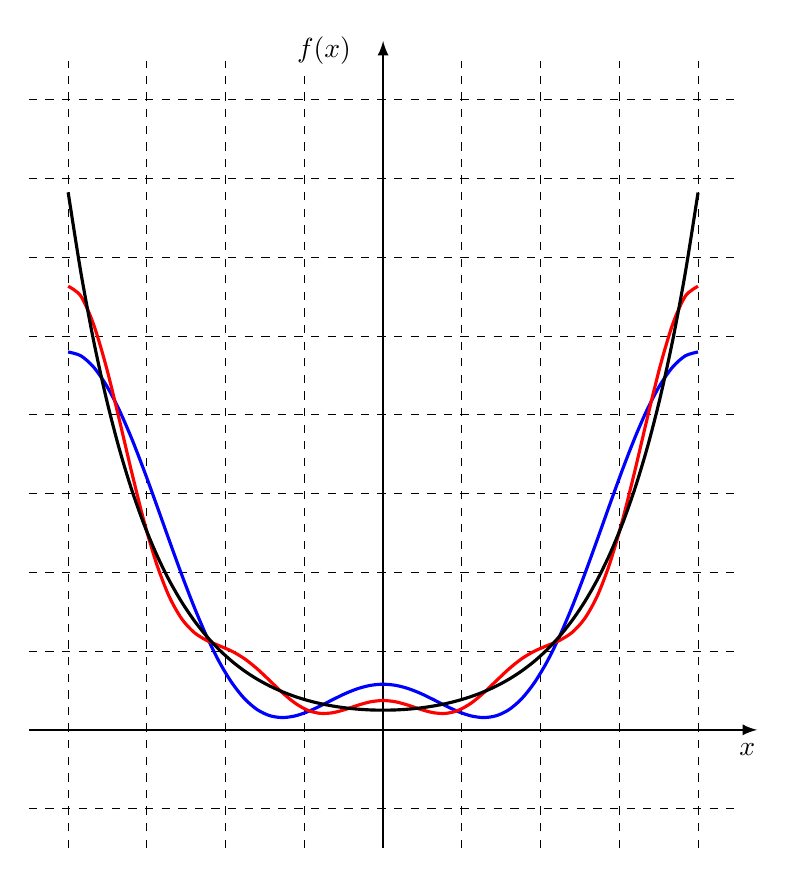
\begin{tikzpicture}
  \draw[-latex,thick] (-4.5,0) -- (4.75,0);
  \node at (4.625,-0.25) {$x$};
  \draw[-latex,thick] (0,-1.5) -- (0,8.75);
  \foreach \x in {-4,...,4}
    \draw[dashed] (\x,-1.5) -- (\x,8.5);
  \foreach \y in {-1,...,8}
    \draw[dashed] (-4.5,\y) -- (4.5,\y);

  \node[fill=white] at (-0.75,8.625) {$f(x)$};
  
  \draw[line width=0.4mm,color=blue] plot[smooth,domain={-4:+4},samples=51]  
  ({\x},{ sinh(4)/16 
          -2*sinh(4)/( 16 + pi^2 * 1^2 ) * cos(deg(1*0.25*pi*\x)) + 2*sinh(4)/( 16 + pi^2 * 2^2 ) * cos(deg(2*0.25*pi*\x)) } );

  \draw[line width=0.4mm,color=red] plot[smooth,domain={-4:+4},samples=51]  
  ({\x},{ sinh(4)/16 
          -2*sinh(4)/( 16 + pi^2 * 1^2 ) * cos(deg(1*0.25*pi*\x)) + 2*sinh(4)/( 16 + pi^2 * 2^2 ) * cos(deg(2*0.25*pi*\x)) 
          -2*sinh(4)/( 16 + pi^2 * 3^2 ) * cos(deg(3*0.25*pi*\x)) + 2*sinh(4)/( 16 + pi^2 * 4^2 ) * cos(deg(4*0.25*pi*\x))} );

  \draw[line width=0.4mm,color=black] plot[smooth,domain={-4:+4},samples=51]  ({\x},{0.25*cosh(\x)});
\end{tikzpicture}
\caption{Illustration of a Fourier series expansion of $f(x) = \cosh(x)/4, -4 \le x \le 4$ for $N = 2$ terms (blue) and $N = 4$ terms (red) with the exact function (black).}
\label{Fig:pde_exampleFourierSeries_HyperbolicCosine}
\end{center}
\end{figure}

The expansion is therefore
\begin{align}
  \frac{1}{L} \cosh(x) &=  \frac{\sinh(L)}{L^2} + \sum_{n=1}^\infty (-1)^n \frac{ 2 \sinh(L) }{ L^2 + n^2 \pi^2 } \cos \left( \frac{n \pi x }{ L } \right) . \nonumber
\end{align}
This is plotted in Fig.~\ref{Fig:pde_exampleFourierSeries_HyperbolicCosine}. The blue and red curves give the approximation of the true function (plotted in black) for $N = 2$ and $N = 4$ terms respectively. It turns out that unlike $f(x) = x$, not very many terms are required to accurately describe the hyperbolic trigonometric functions.

It may seem odd to write out such simple functions in terms of infinite sums of trigonometric functions; however, these were merely simple examples to illustrate the concept of Fourier series expansions. Recall that when it comes to solving second-order partial differential equations, it is often the case that the solutions have no closed form in terms of standard functions and we have no choice but to write those solutions as infinite sums of standard functinos.

Before concluding this discussion, it is worth mentioning that in each of our examples one of either the sine or cosine terms survived with the other vanishing. In first example, $f(x) = x/L$, we have an odd function. Since sine is also an odd function, those terms survive. Conversely, cosine is an even function and those, along with the constant term, vanished. In the second example, we were given an even function, $f(x) = \cosh(x)/L$ and the opposite occurs: the sine terms vanish, and the cosine plus constant terms survive. 

It is often the case that we define our coordinate system for the differential equation so that one of the two sets of terms vanish. To illustrate, if we have the domain $0 \le x \le L$, we can then choose whether to represent a representation based on whether the function is even or odd, which is usually dictated by the boundary conditions. 

For the case where $f(x)$ is odd, i.e., where $f(-x) = -f(x)$ should we temporarily extend the domain to negative values of $x$, i.e., $-L \le x \le 0$, then we all the cosine and constant (even) terms vanish. We can then note that for odd $f(x)$ that
\begin{align}
  \int_{-L}^0 \sin \left( \frac{n \pi x }{ L } \right) f(x) dx = \int_{0}^L \sin \left( \frac{n \pi x }{ L } \right) f(x) dx .
\end{align}
This result is because $f(-x)$ and $\sin(-x)$ are $-f(x)$ and $-\sin(x)$ respectively and the two negatives cancel to make a positive integral. Therefore,
\begin{align}
  a_n &= \frac{1}{L} \int_{-L}^L \sin \left( \frac{n \pi x }{ L } \right) f(x) dx \nonumber \\
      &= \frac{1}{L} \int_{-L}^0 \sin \left( \frac{n \pi x }{ L } \right) f(x) dx + \frac{1}{L} \int_{0}^L \sin \left( \frac{n \pi x }{ L } \right) f(x) dx \nonumber \\
      &= \frac{2}{L} \int_{0}^L \sin \left( \frac{n \pi x }{ L } \right) f(x) dx .
\end{align}
This gives the Fourier expansion of an odd function $f(x)$ on the domain $0 \le x \le L$:
\begin{align}
  f(x) &= \sum_{n=1}^\infty \left[ \frac{2}{L} \int_{0}^L \sin \left( \frac{n \pi x' }{ L } \right) f(x') dx' \right] \sin \left( \frac{n \pi x }{ L } \right)
\end{align}

We can perform a similar analysis for the case where $f(x)$ is even, $f(-x) = f(x)$. The sine terms vanish leaving us with the constant plus cosine terms. This gives
\begin{align}
  c_0 = \frac{1}{2L} \int_{-L}^L f(x) dx = \frac{1}{L} \int_0^L f(x) dx ,
\end{align}
and
\begin{align}
  b_n = \frac{1}{L} \int_{-L}^L \cos \left( \frac{n \pi x }{ L } \right) f(x) dx = \frac{2}{L} \int_0^L  \cos \left( \frac{n \pi x }{ L } \right) f(x) dx .
\end{align}
Therefore, our Fourier expansion for even $f(x)$ on the domain $0 \le x \le L$ is
\begin{align}
  f(x) &= \frac{1}{L} \int_0^L f(x') dx'  + \sum_{n=1}^\infty \left[ \frac{2}{L} \int_{0}^L \cos \left( \frac{n \pi x' }{ L } \right) f(x') dx' \right] \cos \left( \frac{n \pi x }{ L } \right) .
\end{align}

%%%%%%%%%%%%%%%%%%%%%%%%%%%%%%%%%%%%%%%%%%%%%%%%%%%%%%%%%%%%%%%%%%%%%%%%%%%%%%%%%%%%%%%%%%%%%%%
\subsection{Separation of Variables}

The solution technique that we can use to solve many linear second-order partial differential equations is called separation of variables. The technique involves guessing (hoping) that the solution to the partial differential equation can be described as a product of functions that each depend on only one of the independent variables. Given this guess, we insert the form of the solution into the partial differential equation and apply the initial and boundary conditions to check if we can obtain a solution consistent with this assumption. If this is indeed this case, then, since the partial differential equation is linear, we are then guaranteed to have the unique solution.

Given the 1-D heat equation in Cartesian coordinates, we guess that the solution can be written in the form of
\begin{align}
  u(x,t) = X(x) T(t) .
\end{align}
Inserting this into the 1-D heat equation
\begin{align}
  \frac{1}{\alpha} \dho{u}{t} - \dhotwo{u}{x} = 0, \nonumber
\end{align}
gives
\begin{align}
  \frac{X(x)}{\alpha} \dho{}{t}(  T(t) ) - T(t) \dhotwo{}{x} ( X(x) ) = 0 .
\end{align}
Note that we moved the $\alpha$ term to belong to the time term. This is not required; however, it will yield a more convenient form for the solution. Now we divide both sides of the equation by the solution $u = XT$ and rearrange to obtain
\begin{align}
  \frac{1}{\alpha T(t)} \dho{}{t}(T(t)) = \frac{ 1 }{ X(x) } \dhotwo{}{x} ( X(x) ) .
\end{align}
The terms on left-hand side are strictly functions of $t$ and the terms on the right-hand side are strictly functions of $x$. The only way for the left- and right-hand sides of the equation to be equal is if they are both equal to constants:
\begin{subequations}
\begin{align}
  &\frac{1}{\alpha T(t)} \frac{dT}{dt} = C_1 , \\*
  &\frac{1}{X(x)} \frac{d^2 X}{dx^2} = C_2 .
\end{align}
\end{subequations}
These are now written as ordinary differential equations since they only depend upon a single variable. We can show that the constants must be equal by inserting the solution back into the equation.
\begin{align}
  C_1 = C_2 .
\end{align}
The constant could be positive, negative, or even zero in some special cases. Depending on what happens, we will get different forms for the solution. To resolve this further, we need to evaluate the boundary conditions for a specific problem. We now proceed to analyze such a problem.


%%%%%%%%%%%%%%%%%%%%%%%%%%%%%%%%%%%%%%%%%%%%%%%%%%%%%%%%%%%%%%%%%%%%%%%%%%%%%%%%%%%%%%%%%%%%%%%
\subsection{Example: Transient Heat Conduction with Symmetric BCs}

Let us consider the problem of heat conduction on the domain $0 \le x \le L$:
\begin{align}
  \dho{u}{t} - \alpha \nabla^2 u(\pos,t) = 0, \quad u(x,0) = f(x), \quad u(0,t) = u(L,t) = 0 .
\end{align}
Here $u$ describes the temperature of the system, $\alpha$ is the thermal diffusivity (which is the heat conductivity divided by the product of the density and specific heat capacity), an initial arbitrary temperature distribution $f(x)$ is prescribed, and the temperature is held constant at zero at the boundaries for all times.

Applying separation of variables with $u(x,t) = T(t) X(x)$, we get the result
\begin{subequations}
\begin{align}
  &\frac{1}{\alpha T(t)} \frac{dT}{dt} = C , \nonumber \\*
  &\frac{1}{X(x)} \frac{d^2 X}{dx^2} = C . \nonumber
\end{align}
\end{subequations}
Now we have to decide upon the whether $C$ is positive, negative, or zero. For the case where $C$ is zero, the differential equation in $X$ becomes
\begin{align}
  \frac{d^2 X}{dx^2} = 0.
\end{align}
This would yield solutions that is a line 
\begin{align}
  X(x) = A x + B .
\end{align}
The boundary conditions require that the solution go to zero on both ends, so the only solution that would satisfy this would be for the solution to be zero everywhere. This is a trivial solution and not of practical interest, so we reject this case. The case where $C > 0$, we have
\begin{align}
  \frac{d^2 X}{dx^2} - C X(x) = 0.
\end{align}
This would yield exponentials or hyperbolic trigonometric functions: 
\begin{align}
  X(x) = A \sinh ( \sqrt{C} x ) + B \cosh ( \sqrt{C} x ) .
\end{align}
There are no sets of coefficients we could choose to force the solution go to zero at $x = 0$ and $x = L$ except for $A = 0$ and $B = 0$, which is again the trivial solution. We again, reject $C > 0$. Finally, we try a negative value of $C$. For convenience we define
\begin{align}
  C = -k^2
\end{align}
which gives the differential equation
\begin{align}
  \frac{d^2 X}{dx^2} + k^2 X(x) = 0.
\end{align}
This gives the solution
\begin{align}
  X(x) = A \sin( k x ) + B \cos ( k x ) .
\end{align}
Applying our boundary condition at $X(0) = 0$ we have
\begin{align}
  X(0) =  B  = 0 .
\end{align}
Next, applying the boundary condition at $X(L) = $ gives
\begin{align}
  X(L) = A \sin( k L ) = 0 .
\end{align}
Either $A = 0$, which is again the trivial solution, or 
\begin{align}
  k = \frac{n\pi}{L}, \quad n = 1, 2, 3, \ldots
\end{align}
(The negative values of $n$ would yield identical results with the sign flipped, so we leave those out, as they would be redundant.) This implies that there are infinitely many possible solutions to $X(x)$ that satisfy the differential equation and the boundary conditions. Since the equation is linear, we can take the sum of all of the solutions
\begin{align}
  X(x) = \sum_{n=1}^\infty A_n \sin \left( \frac{ n \pi x }{ L } \right) .
\end{align}
Note that by virtue of the boundary conditions $X(x)$ is an odd function if we were to temporarily extend the domain into the negative range.

Now, returning to the time term we have
\begin{align}
  \frac{1}{T} \frac{dT}{dt} = -\alpha k_n^2 .
\end{align}
Here we denoted the constant as $k_n$ to indicate that there are infinitely many values of $k$ that solve the equation. Solving this gives
\begin{align}
  T(t) = K e^{-\alpha k_n^2 t}.
\end{align}
where $K$ is an arbitrary constant.

Multiplying these together, we have 
\begin{align}
  u(x,t) &= X(x) T(t) =  \sum_{n=0}^\infty A_n \sin \left( \frac{ n \pi x }{ L } \right)  K e^{-\alpha k_n^2 t} . \nonumber 
\end{align}
Combining the constants and writing the solution explicitly gives the result:
\begin{align}
  u(x,t) &= \sum_{n=1}^\infty A_n \sin \left( \frac{ n \pi x }{ L } \right)  \exp \left[ -\alpha \left( \frac{ n \pi }{ L } \right)^2 t \right] .
\end{align}

Now there remains the matter of finding the constants $A_n$. This is done by applying the initial condition. We have
\begin{align}
  u(x,0) = f(x) = \sum_{n=1}^\infty A_n \sin \left( \frac{ n \pi x }{ L } \right) .
\end{align}
We can solve for the constants by multiplying by sine functions with different periods, integrating from $0 \le x \le L$.
\begin{align}
  \int_0^L \sin \left( \frac{ m \pi x }{ L } \right) f(x) dx = \sum_{n=1}^\infty A_n \int_0^L \sin \left( \frac{ n \pi x }{ L } \right)  \sin \left( \frac{ m \pi x }{ L } \right) dx .
\end{align}
Applying orthogonality we get
\begin{align}
  \int_0^L \sin \left( \frac{ m \pi x }{ L } \right) f(x) dx = \sum_{n=1}^\infty A_n \frac{L}{2} \delta_{nm}.
\end{align}
The Kronecker delta ensures only the terms with $n = m$ are nonzero. Therefore, we can solve for the coefficient as
\begin{align}
  A_n = \frac{2}{L} \int_0^L \sin \left( \frac{ n \pi x }{ L } \right) f(x) dx .
\end{align}
Note that this is equivalent to the Fourier expansion of $f(x)$ for an odd function on the domain of $0 \le x \le L$.

Therefore, once we are given $f(x)$, we can obtain the coefficients and solution in terms of Fourier expansions. Unless $f(x)$ happens to just so happen to match some combination of sine waves itself, then the best we can do is represent the solution as an infinite sum of sine functions.

\begin{figure}[b!]
\begin{center}
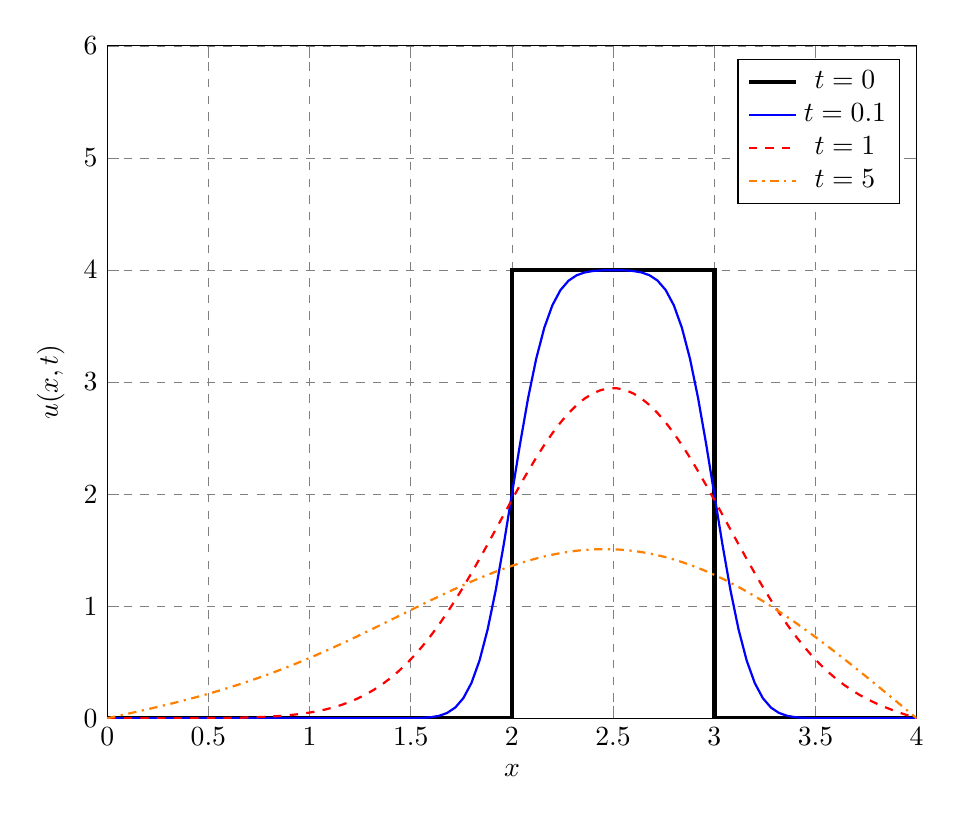
\begin{tikzpicture} \begin{axis}
[scale=1.5,
 xmin=0,  xmax=4,
 ymin=0,  ymax=6,
 grid=major, 
 major grid style={color=gray,line width=0.2pt, dashed},
 xlabel=$x$,
 ylabel={$u(x,t)$}
]

\addplot[line width=0.6mm, color=black] coordinates {
(  0 , 0 )
(  2 , 0 )
(  2 , 4 )
(  3 , 4 )
(  3 , 0 )
(  4 , 0 )
};
\addlegendentry{$t = 0$};

\addplot[line width=0.8pt, color=blue] coordinates {
 ( 0.0000e+00 , 0.0000e+00 ) 
 ( 4.0000e-02 , -9.3737e-17 ) 
 ( 8.0000e-02 , -3.5295e-17 ) 
 ( 1.2000e-01 , -1.6711e-16 ) 
 ( 1.6000e-01 , 5.1285e-17 ) 
 ( 2.0000e-01 , 3.0463e-16 ) 
 ( 2.4000e-01 , 2.4039e-16 ) 
 ( 2.8000e-01 , 3.4846e-16 ) 
 ( 3.2000e-01 , 3.1076e-16 ) 
 ( 3.6000e-01 , 4.5230e-16 ) 
 ( 4.0000e-01 , 2.7041e-16 ) 
 ( 4.4000e-01 , 5.0804e-16 ) 
 ( 4.8000e-01 , 4.3556e-16 ) 
 ( 5.2000e-01 , 3.0051e-17 ) 
 ( 5.6000e-01 , 3.5949e-16 ) 
 ( 6.0000e-01 , 3.6128e-16 ) 
 ( 6.4000e-01 , 2.3353e-16 ) 
 ( 6.8000e-01 , -1.3735e-16 ) 
 ( 7.2000e-01 , 7.9480e-17 ) 
 ( 7.6000e-01 , 3.3879e-16 ) 
 ( 8.0000e-01 , 1.7522e-16 ) 
 ( 8.4000e-01 , 7.6230e-16 ) 
 ( 8.8000e-01 , 4.7901e-15 ) 
 ( 9.2000e-01 , 4.4369e-14 ) 
 ( 9.6000e-01 , 3.8478e-13 ) 
 ( 1.0000e+00 , 3.0750e-12 ) 
 ( 1.0400e+00 , 2.2704e-11 ) 
 ( 1.0800e+00 , 1.5499e-10 ) 
 ( 1.1200e+00 , 9.7834e-10 ) 
 ( 1.1600e+00 , 5.7110e-09 ) 
 ( 1.2000e+00 , 3.0835e-08 ) 
 ( 1.2400e+00 , 1.5401e-07 ) 
 ( 1.2800e+00 , 7.1173e-07 ) 
 ( 1.3200e+00 , 3.0440e-06 ) 
 ( 1.3600e+00 , 1.2052e-05 ) 
 ( 1.4000e+00 , 4.4181e-05 ) 
 ( 1.4400e+00 , 1.5003e-04 ) 
 ( 1.4800e+00 , 4.7207e-04 ) 
 ( 1.5200e+00 , 1.3770e-03 ) 
 ( 1.5600e+00 , 3.7257e-03 ) 
 ( 1.6000e+00 , 9.3555e-03 ) 
 ( 1.6400e+00 , 2.1819e-02 ) 
 ( 1.6800e+00 , 4.7303e-02 ) 
 ( 1.7200e+00 , 9.5430e-02 ) 
 ( 1.7600e+00 , 1.7937e-01 ) 
 ( 1.8000e+00 , 3.1460e-01 ) 
 ( 1.8400e+00 , 5.1580e-01 ) 
 ( 1.8800e+00 , 7.9229e-01 ) 
 ( 1.9200e+00 , 1.1432e+00 ) 
 ( 1.9600e+00 , 1.5546e+00 ) 
 ( 2.0000e+00 , 2.0000e+00 ) 
 ( 2.0400e+00 , 2.4454e+00 ) 
 ( 2.0800e+00 , 2.8568e+00 ) 
 ( 2.1200e+00 , 3.2077e+00 ) 
 ( 2.1600e+00 , 3.4842e+00 ) 
 ( 2.2000e+00 , 3.6854e+00 ) 
 ( 2.2400e+00 , 3.8206e+00 ) 
 ( 2.2800e+00 , 3.9046e+00 ) 
 ( 2.3200e+00 , 3.9527e+00 ) 
 ( 2.3600e+00 , 3.9782e+00 ) 
 ( 2.4000e+00 , 3.9906e+00 ) 
 ( 2.4400e+00 , 3.9961e+00 ) 
 ( 2.4800e+00 , 3.9982e+00 ) 
 ( 2.5200e+00 , 3.9982e+00 ) 
 ( 2.5600e+00 , 3.9961e+00 ) 
 ( 2.6000e+00 , 3.9906e+00 ) 
 ( 2.6400e+00 , 3.9782e+00 ) 
 ( 2.6800e+00 , 3.9527e+00 ) 
 ( 2.7200e+00 , 3.9046e+00 ) 
 ( 2.7600e+00 , 3.8206e+00 ) 
 ( 2.8000e+00 , 3.6854e+00 ) 
 ( 2.8400e+00 , 3.4842e+00 ) 
 ( 2.8800e+00 , 3.2077e+00 ) 
 ( 2.9200e+00 , 2.8568e+00 ) 
 ( 2.9600e+00 , 2.4454e+00 ) 
 ( 3.0000e+00 , 2.0000e+00 ) 
 ( 3.0400e+00 , 1.5546e+00 ) 
 ( 3.0800e+00 , 1.1432e+00 ) 
 ( 3.1200e+00 , 7.9229e-01 ) 
 ( 3.1600e+00 , 5.1580e-01 ) 
 ( 3.2000e+00 , 3.1460e-01 ) 
 ( 3.2400e+00 , 1.7937e-01 ) 
 ( 3.2800e+00 , 9.5430e-02 ) 
 ( 3.3200e+00 , 4.7303e-02 ) 
 ( 3.3600e+00 , 2.1819e-02 ) 
 ( 3.4000e+00 , 9.3555e-03 ) 
 ( 3.4400e+00 , 3.7257e-03 ) 
 ( 3.4800e+00 , 1.3770e-03 ) 
 ( 3.5200e+00 , 4.7207e-04 ) 
 ( 3.5600e+00 , 1.5003e-04 ) 
 ( 3.6000e+00 , 4.4181e-05 ) 
 ( 3.6400e+00 , 1.2052e-05 ) 
 ( 3.6800e+00 , 3.0440e-06 ) 
 ( 3.7200e+00 , 7.1173e-07 ) 
 ( 3.7600e+00 , 1.5401e-07 ) 
 ( 3.8000e+00 , 3.0835e-08 ) 
 ( 3.8400e+00 , 5.7110e-09 ) 
 ( 3.8800e+00 , 9.7834e-10 ) 
 ( 3.9200e+00 , 1.5495e-10 ) 
 ( 3.9600e+00 , 2.2319e-11 ) 
 ( 4.0000e+00 , -3.8448e-17 ) 
};
\addlegendentry{$t = 0.1$};

\addplot[line width=0.8pt, color=red, dashed] coordinates {
 ( 0.0000e+00 , 0.0000e+00 ) 
 ( 4.0000e-02 , 1.3290e-05 ) 
 ( 8.0000e-02 , 2.8609e-05 ) 
 ( 1.2000e-01 , 4.8228e-05 ) 
 ( 1.6000e-01 , 7.4917e-05 ) 
 ( 2.0000e-01 , 1.1225e-04 ) 
 ( 2.4000e-01 , 1.6496e-04 ) 
 ( 2.8000e-01 , 2.3940e-04 ) 
 ( 3.2000e-01 , 3.4405e-04 ) 
 ( 3.6000e-01 , 4.9027e-04 ) 
 ( 4.0000e-01 , 6.9307e-04 ) 
 ( 4.4000e-01 , 9.7221e-04 ) 
 ( 4.8000e-01 , 1.3534e-03 ) 
 ( 5.2000e-01 , 1.8700e-03 ) 
 ( 5.6000e-01 , 2.5642e-03 ) 
 ( 6.0000e-01 , 3.4901e-03 ) 
 ( 6.4000e-01 , 4.7148e-03 ) 
 ( 6.8000e-01 , 6.3220e-03 ) 
 ( 7.2000e-01 , 8.4144e-03 ) 
 ( 7.6000e-01 , 1.1117e-02 ) 
 ( 8.0000e-01 , 1.4579e-02 ) 
 ( 8.4000e-01 , 1.8979e-02 ) 
 ( 8.8000e-01 , 2.4528e-02 ) 
 ( 9.2000e-01 , 3.1468e-02 ) 
 ( 9.6000e-01 , 4.0079e-02 ) 
 ( 1.0000e+00 , 5.0679e-02 ) 
 ( 1.0400e+00 , 6.3623e-02 ) 
 ( 1.0800e+00 , 7.9302e-02 ) 
 ( 1.1200e+00 , 9.8143e-02 ) 
 ( 1.1600e+00 , 1.2060e-01 ) 
 ( 1.2000e+00 , 1.4716e-01 ) 
 ( 1.2400e+00 , 1.7832e-01 ) 
 ( 1.2800e+00 , 2.1457e-01 ) 
 ( 1.3200e+00 , 2.5641e-01 ) 
 ( 1.3600e+00 , 3.0432e-01 ) 
 ( 1.4000e+00 , 3.5873e-01 ) 
 ( 1.4400e+00 , 4.2002e-01 ) 
 ( 1.4800e+00 , 4.8850e-01 ) 
 ( 1.5200e+00 , 5.6439e-01 ) 
 ( 1.5600e+00 , 6.4779e-01 ) 
 ( 1.6000e+00 , 7.3870e-01 ) 
 ( 1.6400e+00 , 8.3694e-01 ) 
 ( 1.6800e+00 , 9.4223e-01 ) 
 ( 1.7200e+00 , 1.0541e+00 ) 
 ( 1.7600e+00 , 1.1719e+00 ) 
 ( 1.8000e+00 , 1.2949e+00 ) 
 ( 1.8400e+00 , 1.4220e+00 ) 
 ( 1.8800e+00 , 1.5524e+00 ) 
 ( 1.9200e+00 , 1.6846e+00 ) 
 ( 1.9600e+00 , 1.8174e+00 ) 
 ( 2.0000e+00 , 1.9493e+00 ) 
 ( 2.0400e+00 , 2.0789e+00 ) 
 ( 2.0800e+00 , 2.2046e+00 ) 
 ( 2.1200e+00 , 2.3249e+00 ) 
 ( 2.1600e+00 , 2.4383e+00 ) 
 ( 2.2000e+00 , 2.5433e+00 ) 
 ( 2.2400e+00 , 2.6385e+00 ) 
 ( 2.2800e+00 , 2.7227e+00 ) 
 ( 2.3200e+00 , 2.7947e+00 ) 
 ( 2.3600e+00 , 2.8535e+00 ) 
 ( 2.4000e+00 , 2.8984e+00 ) 
 ( 2.4400e+00 , 2.9286e+00 ) 
 ( 2.4800e+00 , 2.9439e+00 ) 
 ( 2.5200e+00 , 2.9439e+00 ) 
 ( 2.5600e+00 , 2.9286e+00 ) 
 ( 2.6000e+00 , 2.8984e+00 ) 
 ( 2.6400e+00 , 2.8535e+00 ) 
 ( 2.6800e+00 , 2.7947e+00 ) 
 ( 2.7200e+00 , 2.7227e+00 ) 
 ( 2.7600e+00 , 2.6385e+00 ) 
 ( 2.8000e+00 , 2.5433e+00 ) 
 ( 2.8400e+00 , 2.4383e+00 ) 
 ( 2.8800e+00 , 2.3249e+00 ) 
 ( 2.9200e+00 , 2.2046e+00 ) 
 ( 2.9600e+00 , 2.0789e+00 ) 
 ( 3.0000e+00 , 1.9493e+00 ) 
 ( 3.0400e+00 , 1.8173e+00 ) 
 ( 3.0800e+00 , 1.6845e+00 ) 
 ( 3.1200e+00 , 1.5523e+00 ) 
 ( 3.1600e+00 , 1.4220e+00 ) 
 ( 3.2000e+00 , 1.2947e+00 ) 
 ( 3.2400e+00 , 1.1717e+00 ) 
 ( 3.2800e+00 , 1.0538e+00 ) 
 ( 3.3200e+00 , 9.4188e-01 ) 
 ( 3.3600e+00 , 8.3645e-01 ) 
 ( 3.4000e+00 , 7.3800e-01 ) 
 ( 3.4400e+00 , 6.4682e-01 ) 
 ( 3.4800e+00 , 5.6304e-01 ) 
 ( 3.5200e+00 , 4.8663e-01 ) 
 ( 3.5600e+00 , 4.1746e-01 ) 
 ( 3.6000e+00 , 3.5524e-01 ) 
 ( 3.6400e+00 , 2.9961e-01 ) 
 ( 3.6800e+00 , 2.5009e-01 ) 
 ( 3.7200e+00 , 2.0615e-01 ) 
 ( 3.7600e+00 , 1.6720e-01 ) 
 ( 3.8000e+00 , 1.3258e-01 ) 
 ( 3.8400e+00 , 1.0162e-01 ) 
 ( 3.8800e+00 , 7.3616e-02 ) 
 ( 3.9200e+00 , 4.7834e-02 ) 
 ( 3.9600e+00 , 2.3544e-02 ) 
 ( 4.0000e+00 , 9.0973e-17 ) 
};
\addlegendentry{$t = 1$};

\addplot[line width=0.8pt, color=orange, dash dot] coordinates {
 ( 0.0000e+00 , 0.0000e+00 ) 
 ( 4.0000e-02 , 1.5869e-02 ) 
 ( 8.0000e-02 , 3.1803e-02 ) 
 ( 1.2000e-01 , 4.7866e-02 ) 
 ( 1.6000e-01 , 6.4122e-02 ) 
 ( 2.0000e-01 , 8.0633e-02 ) 
 ( 2.4000e-01 , 9.7461e-02 ) 
 ( 2.8000e-01 , 1.1466e-01 ) 
 ( 3.2000e-01 , 1.3230e-01 ) 
 ( 3.6000e-01 , 1.5043e-01 ) 
 ( 4.0000e-01 , 1.6910e-01 ) 
 ( 4.4000e-01 , 1.8836e-01 ) 
 ( 4.8000e-01 , 2.0827e-01 ) 
 ( 5.2000e-01 , 2.2885e-01 ) 
 ( 5.6000e-01 , 2.5015e-01 ) 
 ( 6.0000e-01 , 2.7221e-01 ) 
 ( 6.4000e-01 , 2.9505e-01 ) 
 ( 6.8000e-01 , 3.1870e-01 ) 
 ( 7.2000e-01 , 3.4318e-01 ) 
 ( 7.6000e-01 , 3.6850e-01 ) 
 ( 8.0000e-01 , 3.9468e-01 ) 
 ( 8.4000e-01 , 4.2171e-01 ) 
 ( 8.8000e-01 , 4.4960e-01 ) 
 ( 9.2000e-01 , 4.7832e-01 ) 
 ( 9.6000e-01 , 5.0787e-01 ) 
 ( 1.0000e+00 , 5.3822e-01 ) 
 ( 1.0400e+00 , 5.6935e-01 ) 
 ( 1.0800e+00 , 6.0120e-01 ) 
 ( 1.1200e+00 , 6.3375e-01 ) 
 ( 1.1600e+00 , 6.6695e-01 ) 
 ( 1.2000e+00 , 7.0072e-01 ) 
 ( 1.2400e+00 , 7.3501e-01 ) 
 ( 1.2800e+00 , 7.6975e-01 ) 
 ( 1.3200e+00 , 8.0486e-01 ) 
 ( 1.3600e+00 , 8.4026e-01 ) 
 ( 1.4000e+00 , 8.7586e-01 ) 
 ( 1.4400e+00 , 9.1156e-01 ) 
 ( 1.4800e+00 , 9.4727e-01 ) 
 ( 1.5200e+00 , 9.8287e-01 ) 
 ( 1.5600e+00 , 1.0183e+00 ) 
 ( 1.6000e+00 , 1.0533e+00 ) 
 ( 1.6400e+00 , 1.0880e+00 ) 
 ( 1.6800e+00 , 1.1220e+00 ) 
 ( 1.7200e+00 , 1.1554e+00 ) 
 ( 1.7600e+00 , 1.1880e+00 ) 
 ( 1.8000e+00 , 1.2197e+00 ) 
 ( 1.8400e+00 , 1.2503e+00 ) 
 ( 1.8800e+00 , 1.2798e+00 ) 
 ( 1.9200e+00 , 1.3080e+00 ) 
 ( 1.9600e+00 , 1.3347e+00 ) 
 ( 2.0000e+00 , 1.3600e+00 ) 
 ( 2.0400e+00 , 1.3836e+00 ) 
 ( 2.0800e+00 , 1.4055e+00 ) 
 ( 2.1200e+00 , 1.4255e+00 ) 
 ( 2.1600e+00 , 1.4436e+00 ) 
 ( 2.2000e+00 , 1.4596e+00 ) 
 ( 2.2400e+00 , 1.4736e+00 ) 
 ( 2.2800e+00 , 1.4853e+00 ) 
 ( 2.3200e+00 , 1.4948e+00 ) 
 ( 2.3600e+00 , 1.5019e+00 ) 
 ( 2.4000e+00 , 1.5066e+00 ) 
 ( 2.4400e+00 , 1.5090e+00 ) 
 ( 2.4800e+00 , 1.5088e+00 ) 
 ( 2.5200e+00 , 1.5061e+00 ) 
 ( 2.5600e+00 , 1.5009e+00 ) 
 ( 2.6000e+00 , 1.4932e+00 ) 
 ( 2.6400e+00 , 1.4830e+00 ) 
 ( 2.6800e+00 , 1.4702e+00 ) 
 ( 2.7200e+00 , 1.4549e+00 ) 
 ( 2.7600e+00 , 1.4370e+00 ) 
 ( 2.8000e+00 , 1.4167e+00 ) 
 ( 2.8400e+00 , 1.3940e+00 ) 
 ( 2.8800e+00 , 1.3689e+00 ) 
 ( 2.9200e+00 , 1.3415e+00 ) 
 ( 2.9600e+00 , 1.3117e+00 ) 
 ( 3.0000e+00 , 1.2798e+00 ) 
 ( 3.0400e+00 , 1.2457e+00 ) 
 ( 3.0800e+00 , 1.2095e+00 ) 
 ( 3.1200e+00 , 1.1713e+00 ) 
 ( 3.1600e+00 , 1.1312e+00 ) 
 ( 3.2000e+00 , 1.0892e+00 ) 
 ( 3.2400e+00 , 1.0455e+00 ) 
 ( 3.2800e+00 , 1.0001e+00 ) 
 ( 3.3200e+00 , 9.5308e-01 ) 
 ( 3.3600e+00 , 9.0461e-01 ) 
 ( 3.4000e+00 , 8.5473e-01 ) 
 ( 3.4400e+00 , 8.0355e-01 ) 
 ( 3.4800e+00 , 7.5116e-01 ) 
 ( 3.5200e+00 , 6.9764e-01 ) 
 ( 3.5600e+00 , 6.4308e-01 ) 
 ( 3.6000e+00 , 5.8758e-01 ) 
 ( 3.6400e+00 , 5.3122e-01 ) 
 ( 3.6800e+00 , 4.7411e-01 ) 
 ( 3.7200e+00 , 4.1631e-01 ) 
 ( 3.7600e+00 , 3.5792e-01 ) 
 ( 3.8000e+00 , 2.9904e-01 ) 
 ( 3.8400e+00 , 2.3973e-01 ) 
 ( 3.8800e+00 , 1.8009e-01 ) 
 ( 3.9200e+00 , 1.2020e-01 ) 
 ( 3.9600e+00 , 6.0140e-02 ) 
 ( 4.0000e+00 , 2.3449e-16 ) 
};
\addlegendentry{$t = 5$};

\end{axis}
\end{tikzpicture}

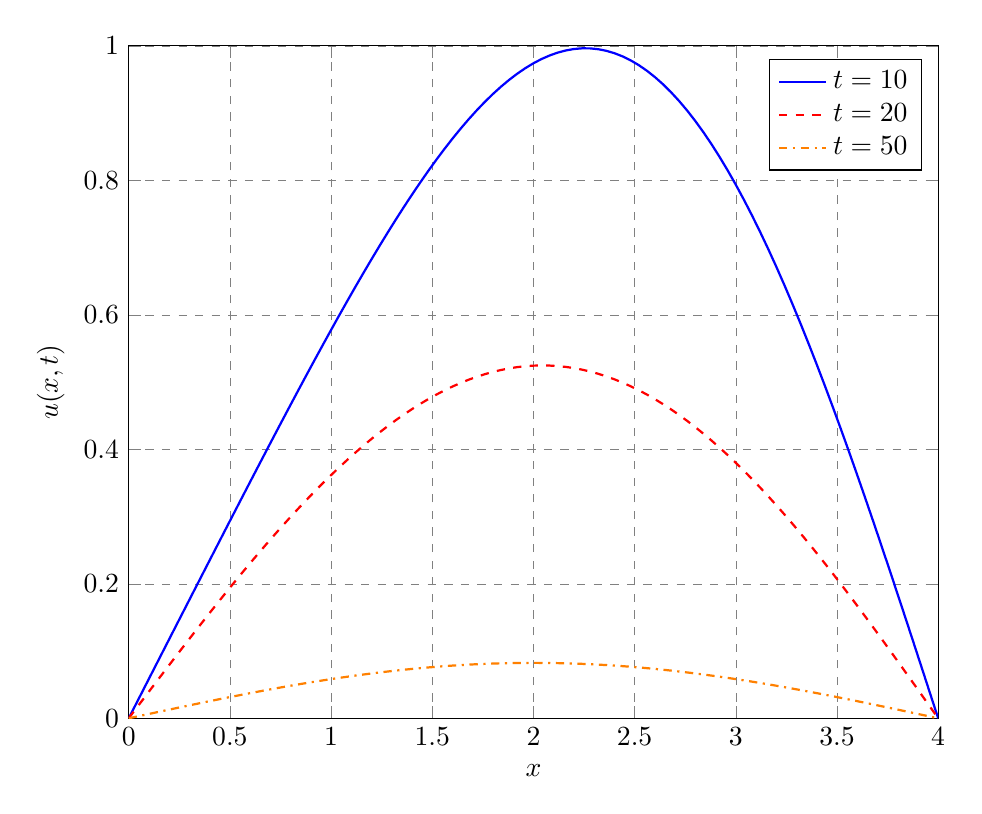
\begin{tikzpicture} \begin{axis}
[scale=1.5,
 xmin=0,  xmax=4,
 ymin=0,  ymax=1,
 grid=major, 
 major grid style={color=gray,line width=0.2pt, dashed},
 xlabel=$x$,
 ylabel={$u(x,t)$}
]

\addplot[line width=0.8pt, color=blue] coordinates {
 ( 0.0000e+00 , 0.0000e+00 ) 
 ( 4.0000e-02 , 2.3531e-02 ) 
 ( 8.0000e-02 , 4.7060e-02 ) 
 ( 1.2000e-01 , 7.0586e-02 ) 
 ( 1.6000e-01 , 9.4107e-02 ) 
 ( 2.0000e-01 , 1.1762e-01 ) 
 ( 2.4000e-01 , 1.4113e-01 ) 
 ( 2.8000e-01 , 1.6462e-01 ) 
 ( 3.2000e-01 , 1.8809e-01 ) 
 ( 3.6000e-01 , 2.1155e-01 ) 
 ( 4.0000e-01 , 2.3498e-01 ) 
 ( 4.4000e-01 , 2.5838e-01 ) 
 ( 4.8000e-01 , 2.8175e-01 ) 
 ( 5.2000e-01 , 3.0507e-01 ) 
 ( 5.6000e-01 , 3.2834e-01 ) 
 ( 6.0000e-01 , 3.5155e-01 ) 
 ( 6.4000e-01 , 3.7468e-01 ) 
 ( 6.8000e-01 , 3.9774e-01 ) 
 ( 7.2000e-01 , 4.2070e-01 ) 
 ( 7.6000e-01 , 4.4355e-01 ) 
 ( 8.0000e-01 , 4.6628e-01 ) 
 ( 8.4000e-01 , 4.8887e-01 ) 
 ( 8.8000e-01 , 5.1130e-01 ) 
 ( 9.2000e-01 , 5.3356e-01 ) 
 ( 9.6000e-01 , 5.5562e-01 ) 
 ( 1.0000e+00 , 5.7747e-01 ) 
 ( 1.0400e+00 , 5.9908e-01 ) 
 ( 1.0800e+00 , 6.2043e-01 ) 
 ( 1.1200e+00 , 6.4149e-01 ) 
 ( 1.1600e+00 , 6.6225e-01 ) 
 ( 1.2000e+00 , 6.8267e-01 ) 
 ( 1.2400e+00 , 7.0272e-01 ) 
 ( 1.2800e+00 , 7.2239e-01 ) 
 ( 1.3200e+00 , 7.4163e-01 ) 
 ( 1.3600e+00 , 7.6042e-01 ) 
 ( 1.4000e+00 , 7.7873e-01 ) 
 ( 1.4400e+00 , 7.9653e-01 ) 
 ( 1.4800e+00 , 8.1379e-01 ) 
 ( 1.5200e+00 , 8.3047e-01 ) 
 ( 1.5600e+00 , 8.4654e-01 ) 
 ( 1.6000e+00 , 8.6198e-01 ) 
 ( 1.6400e+00 , 8.7674e-01 ) 
 ( 1.6800e+00 , 8.9079e-01 ) 
 ( 1.7200e+00 , 9.0411e-01 ) 
 ( 1.7600e+00 , 9.1666e-01 ) 
 ( 1.8000e+00 , 9.2840e-01 ) 
 ( 1.8400e+00 , 9.3932e-01 ) 
 ( 1.8800e+00 , 9.4936e-01 ) 
 ( 1.9200e+00 , 9.5852e-01 ) 
 ( 1.9600e+00 , 9.6675e-01 ) 
 ( 2.0000e+00 , 9.7403e-01 ) 
 ( 2.0400e+00 , 9.8032e-01 ) 
 ( 2.0800e+00 , 9.8562e-01 ) 
 ( 2.1200e+00 , 9.8988e-01 ) 
 ( 2.1600e+00 , 9.9308e-01 ) 
 ( 2.2000e+00 , 9.9521e-01 ) 
 ( 2.2400e+00 , 9.9625e-01 ) 
 ( 2.2800e+00 , 9.9616e-01 ) 
 ( 2.3200e+00 , 9.9494e-01 ) 
 ( 2.3600e+00 , 9.9257e-01 ) 
 ( 2.4000e+00 , 9.8904e-01 ) 
 ( 2.4400e+00 , 9.8433e-01 ) 
 ( 2.4800e+00 , 9.7843e-01 ) 
 ( 2.5200e+00 , 9.7135e-01 ) 
 ( 2.5600e+00 , 9.6306e-01 ) 
 ( 2.6000e+00 , 9.5357e-01 ) 
 ( 2.6400e+00 , 9.4288e-01 ) 
 ( 2.6800e+00 , 9.3098e-01 ) 
 ( 2.7200e+00 , 9.1789e-01 ) 
 ( 2.7600e+00 , 9.0360e-01 ) 
 ( 2.8000e+00 , 8.8813e-01 ) 
 ( 2.8400e+00 , 8.7148e-01 ) 
 ( 2.8800e+00 , 8.5367e-01 ) 
 ( 2.9200e+00 , 8.3471e-01 ) 
 ( 2.9600e+00 , 8.1462e-01 ) 
 ( 3.0000e+00 , 7.9342e-01 ) 
 ( 3.0400e+00 , 7.7113e-01 ) 
 ( 3.0800e+00 , 7.4778e-01 ) 
 ( 3.1200e+00 , 7.2338e-01 ) 
 ( 3.1600e+00 , 6.9797e-01 ) 
 ( 3.2000e+00 , 6.7159e-01 ) 
 ( 3.2400e+00 , 6.4425e-01 ) 
 ( 3.2800e+00 , 6.1600e-01 ) 
 ( 3.3200e+00 , 5.8687e-01 ) 
 ( 3.3600e+00 , 5.5690e-01 ) 
 ( 3.4000e+00 , 5.2613e-01 ) 
 ( 3.4400e+00 , 4.9460e-01 ) 
 ( 3.4800e+00 , 4.6236e-01 ) 
 ( 3.5200e+00 , 4.2945e-01 ) 
 ( 3.5600e+00 , 3.9591e-01 ) 
 ( 3.6000e+00 , 3.6179e-01 ) 
 ( 3.6400e+00 , 3.2714e-01 ) 
 ( 3.6800e+00 , 2.9202e-01 ) 
 ( 3.7200e+00 , 2.5646e-01 ) 
 ( 3.7600e+00 , 2.2053e-01 ) 
 ( 3.8000e+00 , 1.8428e-01 ) 
 ( 3.8400e+00 , 1.4775e-01 ) 
 ( 3.8800e+00 , 1.1100e-01 ) 
 ( 3.9200e+00 , 7.4094e-02 ) 
 ( 3.9600e+00 , 3.7074e-02 ) 
 ( 4.0000e+00 , 1.4456e-16 ) 
};
\addlegendentry{$t = 10$};

\addplot[line width=0.8pt, color=red, dashed] coordinates {
 ( 0.0000e+00 , 0.0000e+00 ) 
 ( 4.0000e-02 , 1.5895e-02 ) 
 ( 8.0000e-02 , 3.1776e-02 ) 
 ( 1.2000e-01 , 4.7629e-02 ) 
 ( 1.6000e-01 , 6.3440e-02 ) 
 ( 2.0000e-01 , 7.9195e-02 ) 
 ( 2.4000e-01 , 9.4881e-02 ) 
 ( 2.8000e-01 , 1.1048e-01 ) 
 ( 3.2000e-01 , 1.2599e-01 ) 
 ( 3.6000e-01 , 1.4138e-01 ) 
 ( 4.0000e-01 , 1.5665e-01 ) 
 ( 4.4000e-01 , 1.7178e-01 ) 
 ( 4.8000e-01 , 1.8676e-01 ) 
 ( 5.2000e-01 , 2.0157e-01 ) 
 ( 5.6000e-01 , 2.1620e-01 ) 
 ( 6.0000e-01 , 2.3064e-01 ) 
 ( 6.4000e-01 , 2.4488e-01 ) 
 ( 6.8000e-01 , 2.5889e-01 ) 
 ( 7.2000e-01 , 2.7268e-01 ) 
 ( 7.6000e-01 , 2.8622e-01 ) 
 ( 8.0000e-01 , 2.9950e-01 ) 
 ( 8.4000e-01 , 3.1251e-01 ) 
 ( 8.8000e-01 , 3.2524e-01 ) 
 ( 9.2000e-01 , 3.3768e-01 ) 
 ( 9.6000e-01 , 3.4981e-01 ) 
 ( 1.0000e+00 , 3.6162e-01 ) 
 ( 1.0400e+00 , 3.7310e-01 ) 
 ( 1.0800e+00 , 3.8424e-01 ) 
 ( 1.1200e+00 , 3.9503e-01 ) 
 ( 1.1600e+00 , 4.0546e-01 ) 
 ( 1.2000e+00 , 4.1551e-01 ) 
 ( 1.2400e+00 , 4.2518e-01 ) 
 ( 1.2800e+00 , 4.3445e-01 ) 
 ( 1.3200e+00 , 4.4332e-01 ) 
 ( 1.3600e+00 , 4.5178e-01 ) 
 ( 1.4000e+00 , 4.5981e-01 ) 
 ( 1.4400e+00 , 4.6741e-01 ) 
 ( 1.4800e+00 , 4.7457e-01 ) 
 ( 1.5200e+00 , 4.8128e-01 ) 
 ( 1.5600e+00 , 4.8754e-01 ) 
 ( 1.6000e+00 , 4.9333e-01 ) 
 ( 1.6400e+00 , 4.9865e-01 ) 
 ( 1.6800e+00 , 5.0349e-01 ) 
 ( 1.7200e+00 , 5.0785e-01 ) 
 ( 1.7600e+00 , 5.1172e-01 ) 
 ( 1.8000e+00 , 5.1509e-01 ) 
 ( 1.8400e+00 , 5.1796e-01 ) 
 ( 1.8800e+00 , 5.2033e-01 ) 
 ( 1.9200e+00 , 5.2219e-01 ) 
 ( 1.9600e+00 , 5.2354e-01 ) 
 ( 2.0000e+00 , 5.2438e-01 ) 
 ( 2.0400e+00 , 5.2469e-01 ) 
 ( 2.0800e+00 , 5.2449e-01 ) 
 ( 2.1200e+00 , 5.2376e-01 ) 
 ( 2.1600e+00 , 5.2252e-01 ) 
 ( 2.2000e+00 , 5.2075e-01 ) 
 ( 2.2400e+00 , 5.1846e-01 ) 
 ( 2.2800e+00 , 5.1565e-01 ) 
 ( 2.3200e+00 , 5.1231e-01 ) 
 ( 2.3600e+00 , 5.0846e-01 ) 
 ( 2.4000e+00 , 5.0409e-01 ) 
 ( 2.4400e+00 , 4.9921e-01 ) 
 ( 2.4800e+00 , 4.9382e-01 ) 
 ( 2.5200e+00 , 4.8792e-01 ) 
 ( 2.5600e+00 , 4.8152e-01 ) 
 ( 2.6000e+00 , 4.7462e-01 ) 
 ( 2.6400e+00 , 4.6724e-01 ) 
 ( 2.6800e+00 , 4.5937e-01 ) 
 ( 2.7200e+00 , 4.5102e-01 ) 
 ( 2.7600e+00 , 4.4221e-01 ) 
 ( 2.8000e+00 , 4.3293e-01 ) 
 ( 2.8400e+00 , 4.2320e-01 ) 
 ( 2.8800e+00 , 4.1302e-01 ) 
 ( 2.9200e+00 , 4.0241e-01 ) 
 ( 2.9600e+00 , 3.9138e-01 ) 
 ( 3.0000e+00 , 3.7993e-01 ) 
 ( 3.0400e+00 , 3.6809e-01 ) 
 ( 3.0800e+00 , 3.5585e-01 ) 
 ( 3.1200e+00 , 3.4323e-01 ) 
 ( 3.1600e+00 , 3.3025e-01 ) 
 ( 3.2000e+00 , 3.1692e-01 ) 
 ( 3.2400e+00 , 3.0324e-01 ) 
 ( 3.2800e+00 , 2.8925e-01 ) 
 ( 3.3200e+00 , 2.7494e-01 ) 
 ( 3.3600e+00 , 2.6034e-01 ) 
 ( 3.4000e+00 , 2.4546e-01 ) 
 ( 3.4400e+00 , 2.3031e-01 ) 
 ( 3.4800e+00 , 2.1492e-01 ) 
 ( 3.5200e+00 , 1.9929e-01 ) 
 ( 3.5600e+00 , 1.8345e-01 ) 
 ( 3.6000e+00 , 1.6741e-01 ) 
 ( 3.6400e+00 , 1.5119e-01 ) 
 ( 3.6800e+00 , 1.3481e-01 ) 
 ( 3.7200e+00 , 1.1828e-01 ) 
 ( 3.7600e+00 , 1.0162e-01 ) 
 ( 3.8000e+00 , 8.4855e-02 ) 
 ( 3.8400e+00 , 6.7995e-02 ) 
 ( 3.8800e+00 , 5.1061e-02 ) 
 ( 3.9200e+00 , 3.4071e-02 ) 
 ( 3.9600e+00 , 1.7045e-02 ) 
 ( 4.0000e+00 , 6.6456e-17 ) 
};
\addlegendentry{$t = 20$};

\addplot[line width=0.8pt, color=orange, dash dot] coordinates {
 ( 0.0000e+00 , 0.0000e+00 ) 
 ( 4.0000e-02 , 2.5880e-03 ) 
 ( 8.0000e-02 , 5.1735e-03 ) 
 ( 1.2000e-01 , 7.7539e-03 ) 
 ( 1.6000e-01 , 1.0327e-02 ) 
 ( 2.0000e-01 , 1.2889e-02 ) 
 ( 2.4000e-01 , 1.5439e-02 ) 
 ( 2.8000e-01 , 1.7974e-02 ) 
 ( 3.2000e-01 , 2.0491e-02 ) 
 ( 3.6000e-01 , 2.2987e-02 ) 
 ( 4.0000e-01 , 2.5461e-02 ) 
 ( 4.4000e-01 , 2.7910e-02 ) 
 ( 4.8000e-01 , 3.0331e-02 ) 
 ( 5.2000e-01 , 3.2723e-02 ) 
 ( 5.6000e-01 , 3.5082e-02 ) 
 ( 6.0000e-01 , 3.7406e-02 ) 
 ( 6.4000e-01 , 3.9694e-02 ) 
 ( 6.8000e-01 , 4.1942e-02 ) 
 ( 7.2000e-01 , 4.4150e-02 ) 
 ( 7.6000e-01 , 4.6313e-02 ) 
 ( 8.0000e-01 , 4.8431e-02 ) 
 ( 8.4000e-01 , 5.0501e-02 ) 
 ( 8.8000e-01 , 5.2521e-02 ) 
 ( 9.2000e-01 , 5.4490e-02 ) 
 ( 9.6000e-01 , 5.6404e-02 ) 
 ( 1.0000e+00 , 5.8263e-02 ) 
 ( 1.0400e+00 , 6.0065e-02 ) 
 ( 1.0800e+00 , 6.1807e-02 ) 
 ( 1.1200e+00 , 6.3488e-02 ) 
 ( 1.1600e+00 , 6.5107e-02 ) 
 ( 1.2000e+00 , 6.6661e-02 ) 
 ( 1.2400e+00 , 6.8150e-02 ) 
 ( 1.2800e+00 , 6.9572e-02 ) 
 ( 1.3200e+00 , 7.0924e-02 ) 
 ( 1.3600e+00 , 7.2207e-02 ) 
 ( 1.4000e+00 , 7.3419e-02 ) 
 ( 1.4400e+00 , 7.4558e-02 ) 
 ( 1.4800e+00 , 7.5623e-02 ) 
 ( 1.5200e+00 , 7.6614e-02 ) 
 ( 1.5600e+00 , 7.7529e-02 ) 
 ( 1.6000e+00 , 7.8368e-02 ) 
 ( 1.6400e+00 , 7.9130e-02 ) 
 ( 1.6800e+00 , 7.9813e-02 ) 
 ( 1.7200e+00 , 8.0418e-02 ) 
 ( 1.7600e+00 , 8.0943e-02 ) 
 ( 1.8000e+00 , 8.1388e-02 ) 
 ( 1.8400e+00 , 8.1753e-02 ) 
 ( 1.8800e+00 , 8.2038e-02 ) 
 ( 1.9200e+00 , 8.2241e-02 ) 
 ( 1.9600e+00 , 8.2364e-02 ) 
 ( 2.0000e+00 , 8.2405e-02 ) 
 ( 2.0400e+00 , 8.2364e-02 ) 
 ( 2.0800e+00 , 8.2243e-02 ) 
 ( 2.1200e+00 , 8.2040e-02 ) 
 ( 2.1600e+00 , 8.1756e-02 ) 
 ( 2.2000e+00 , 8.1392e-02 ) 
 ( 2.2400e+00 , 8.0947e-02 ) 
 ( 2.2800e+00 , 8.0422e-02 ) 
 ( 2.3200e+00 , 7.9818e-02 ) 
 ( 2.3600e+00 , 7.9136e-02 ) 
 ( 2.4000e+00 , 7.8375e-02 ) 
 ( 2.4400e+00 , 7.7537e-02 ) 
 ( 2.4800e+00 , 7.6622e-02 ) 
 ( 2.5200e+00 , 7.5631e-02 ) 
 ( 2.5600e+00 , 7.4566e-02 ) 
 ( 2.6000e+00 , 7.3428e-02 ) 
 ( 2.6400e+00 , 7.2216e-02 ) 
 ( 2.6800e+00 , 7.0934e-02 ) 
 ( 2.7200e+00 , 6.9582e-02 ) 
 ( 2.7600e+00 , 6.8160e-02 ) 
 ( 2.8000e+00 , 6.6672e-02 ) 
 ( 2.8400e+00 , 6.5118e-02 ) 
 ( 2.8800e+00 , 6.3499e-02 ) 
 ( 2.9200e+00 , 6.1818e-02 ) 
 ( 2.9600e+00 , 6.0076e-02 ) 
 ( 3.0000e+00 , 5.8274e-02 ) 
 ( 3.0400e+00 , 5.6415e-02 ) 
 ( 3.0800e+00 , 5.4501e-02 ) 
 ( 3.1200e+00 , 5.2532e-02 ) 
 ( 3.1600e+00 , 5.0512e-02 ) 
 ( 3.2000e+00 , 4.8442e-02 ) 
 ( 3.2400e+00 , 4.6323e-02 ) 
 ( 3.2800e+00 , 4.4160e-02 ) 
 ( 3.3200e+00 , 4.1952e-02 ) 
 ( 3.3600e+00 , 3.9703e-02 ) 
 ( 3.4000e+00 , 3.7415e-02 ) 
 ( 3.4400e+00 , 3.5091e-02 ) 
 ( 3.4800e+00 , 3.2731e-02 ) 
 ( 3.5200e+00 , 3.0339e-02 ) 
 ( 3.5600e+00 , 2.7917e-02 ) 
 ( 3.6000e+00 , 2.5468e-02 ) 
 ( 3.6400e+00 , 2.2993e-02 ) 
 ( 3.6800e+00 , 2.0496e-02 ) 
 ( 3.7200e+00 , 1.7978e-02 ) 
 ( 3.7600e+00 , 1.5443e-02 ) 
 ( 3.8000e+00 , 1.2893e-02 ) 
 ( 3.8400e+00 , 1.0329e-02 ) 
 ( 3.8800e+00 , 7.7560e-03 ) 
 ( 3.9200e+00 , 5.1749e-03 ) 
 ( 3.9600e+00 , 2.5887e-03 ) 
 ( 4.0000e+00 , 1.0093e-17 ) 
};
\addlegendentry{$t = 50$};

\end{axis}
\end{tikzpicture}

\caption{Plot of transient heat conduction for (top) early time and (bottom) late times.}
\label{Fig:pde_transientHeatCondution_Example}
\end{center}
\end{figure}



Let us illustrate this with an example. The domain is $L = 4$ and $\alpha = 0.1$ and the initial condition is
\begin{align}
  f(x) = \left\{ \begin{array}{r l}
  4, & \quad 2 \le x \le 3 \\
  0, & \quad \text{otherwise} \\ \end{array} \right. .
\end{align}
The Fourier expansion for these coefficients are
\begin{align}
  A_n &= 2 \int_2^3 \sin \left( \frac{ n \pi x }{ 4 } \right) dx \nonumber \\
      &= \frac{8}{n\pi} \left[ \cos \left( \frac{n\pi}{2} \right) - \cos \left( \frac{ 3n\pi }{ 4 } \right) \right] .
\end{align}
Because the function is discontinuous, we will require a very large number of coefficients to accurately represent the solution. The computations were done using a computer with $N = 1000$ coefficients. Fig.~\ref{Fig:pde_transientHeatCondution_Example} provides plots of the solution at early times and later times. The early times show the initial condition spreading out in a diffusive process. Eventually, the shape of the solution begins to be significantly impacted by the boundary conditions. At later times, the solution evolves into a single exponentially decaying sine wave. This is because of the 
\begin{align}
   \exp \left[ -\alpha \left( \frac{ n \pi }{ L } \right)^2 t \right] \nonumber
\end{align}
term. For large $t$ the argument of the exponential becomes large making the exponential term small. Because the exponent is proportional to $n^2$, as $t$ gets large, the terms for $n = 2, 3, \ldots$ make the exponent increasingly large, making the overall exponential vanishingly small. For late times the $n = 1$ term dominates the others and we are left with a single sine wave.


%%%%%%%%%%%%%%%%%%%%%%%%%%%%%%%%%%%%%%%%%%%%%%%%%%%%%%%%%%%%%%%%%%%%%%%%%%%%%%%%%%%%%%%%%%%%%%%
\subsection{Example: Transient 1-D Neutron Diffusion and Criticality}

The time-dependent neutron diffusion equation is
\begin{align}
  \frac{1}{v} \dho{u}{t} - D \dhotwo{u}{x} + \Sigma_a u(x,t) = \nu \Sigma_f u(x,t) , \quad u(x,0) = f(x), \quad u(0,t) = u(L,t) = 0 .
\end{align}
Here $u$ represents the path-length density of neutrons, $v$ is the neutron speed, $D$ is the neutron diffusion coefficient, $\Sigma_a$ is the absorption coefficient (macroscopic cross section), $\nu$ is the mean number of neutrons produced from fission, and $\Sigma_f$ is the fission coefficient. We specify an initial condition for the neutrons $f(x)$ and require that the neutron distribution goes to zero on the edges. In practice, we have more sophisticated boundary conditions, but these complicate matters significantly and are beyond the scope of this section.

Before proceeding, let us first consider the difference of the neutron diffusion equation from the heat conduction equation. These differences are primarily the addition of absorption (loss) and fission (gain) terms. In the heat conduction problem we had no mechanism for thermal energy to be created or destroyed (e.g., converted into or from chemical energy through endothermic or exothermic chemical reactions).

We first rearrange the equation by dividing by the diffusion coefficient and move the absorption term to the right-hand side
\begin{align}
  \frac{1}{v D} \dho{u}{t} - \dhotwo{u}{x} = \frac{ \nu \Sigma_f - \Sigma_a }{ D } u(x,t) .
\end{align}
As with the transient heat conduction problem, we assume the solution is separable of the form
\begin{align}
  u(x,t) = X(x) T(t) ,
\end{align}
insert this into the differential equation, and divide by $u$ to obtain
\begin{align}
  \frac{1}{v D T} \frac{dT}{dt} - \frac{1}{X} \frac{d^2 X}{dx^2} = \frac{ \nu \Sigma_f - \Sigma_a }{ D } .
\end{align}
We now have an equation where the right-hand side is equal to a constant and the time and space terms are only dependent on the time and space variables. Therefore, we can assert that the solutions are constants. As with the heat conduction, we need to analyze the possibilities. We will skip this step here and provide the one that will work and make the next steps easiest. We state that
\begin{subequations}
\begin{align}
  \frac{1}{vD T} \frac{dT}{dt} &= \frac{ \nu \Sigma_f - \Sigma_a }{ D } - B^2, \\
  \frac{1}{X} \frac{d^2 X}{dx^2} &= -B^2 .
\end{align}
\end{subequations}
Here $B^2$ is some constant for which we will find valid solutions. (This coefficient is referred to as the buckling, as it follows similar mathematics to structure mechanics, but otherwise has no physical connection.) 

As for the heat conduction problem, the spatial function $X$ depends upon the trigonometric functions
\begin{align}
  X(x) = A \sin ( Bx ) + C \cos ( Bx ) .
\end{align}
Applying the boundary conditions $X(0) = X(L) = 0$ yields the same results as before:
\begin{subequations}
\begin{align}
  C &= 0, \\
  A &= \frac{n\pi}{L}, \quad n = 1, 2, 3, \ldots
\end{align}
\end{subequations}
Therefore, we have obtained infinitely many solutions to the $X$ equation and can take a linear combination as with the heat conduction problem:
\begin{align}
  X(x) = \sum_{n=1}^\infty A_n \sin \left( \frac{ n \pi x }{ L } \right) .
\end{align}
Again, each term in the summation has a different constant coefficient.

The time term is obtained in a similar process, but now as a more complicated form
\begin{align}
  T(t) = K \exp \left[ \left( \nu \Sigma_f - \Sigma_a - \left( \frac{n \pi}{L} \right)^2 D \right) vt \right] .
\end{align}
The values in the exponential will have a significant impact on the time-evolution and criticality of the system. 

Multiplying the space and time terms together and combining constants gives the solution for 1-D transient neutron diffusion
\begin{align}
  u(x,t) = \sum_{n=1}^\infty A_n \sin \left( \frac{ n \pi x }{ L } \right) \exp \left[ \left( \nu \Sigma_f - \Sigma_a - \left( \frac{n \pi}{L} \right)^2 D \right) v t \right]  .
\end{align}

The major difference with the heat conduction equation is in the exponential term for the time behavior. Namely, we have the term
\begin{align}
   \nu \Sigma_f - \Sigma_a - \left( \frac{n \pi}{L} \right)^2 D \nonumber
\end{align}
which gives the production coefficient for fission, the loss coefficient for absorption, and a third term that is a loss term proportional to the neutron diffusion coefficient divided by the length of the reactor squared. The last term describes the physical phenomenon of leakage of neutrons from the system. Note that the least negative of these terms has $n = 1$ and, as we saw with the heat conduction problem, will be the term that survives the longest. We can state that if
\begin{align}
  \nu \Sigma_f = \Sigma_a + \left( \frac{\pi}{L} \right)^2 D  \nonumber
\end{align}
then the largest exponential term will be zero with all others negative. This is referred to as a critical reactor and implies that after long times the neutron distribution will reach a steady state sine wave distribution. The case where
\begin{align}
  \nu \Sigma_f < \Sigma_a + \left( \frac{\pi}{L} \right)^2 D  \nonumber
\end{align}
corresponds to a subcritical reactor. This means that the neutron population will reach a sine wave that is decaying exponentially in time, which is what we saw for the heat conduction problem. Finally, we have the case where
\begin{align}
  \nu \Sigma_f > \Sigma_a + \left( \frac{\pi}{L} \right)^2 D . \nonumber
\end{align}
This is the supercritical configuration, which corresponds to a long time solution that is a sine wave that grows exponentially with time. 


%%%%%%%%%%%%%%%%%%%%%%%%%%%%%%%%%%%%%%%%%%%%%%%%%%%%%%%%%%%%%%%%%%%%%%%%%%%%%%%%%%%%%%%%%%%%%%%
\subsection{Superposition}

The two previous examples had zero boundary conditions and no inhomogeneous term. This simplified the analysis significantly. Now suppose instead we have boundary conditions that are not zero on both sides, but nonzero and potentially asymmetric. In these cases, we may not be able to easily find solutions that simultaneously satisfy all the conditions. Fortunately, because the heat equation is linear, we can apply the principle of superposition. The idea is rather than solving the entire problem at once, to break it up into simpler problems, combine the results, and then find values of the coefficients. We have seen similar analysis before in finding homogeneous and particular solutions of ordinary differential equations.

For the transient heat equation, we may split the solution into two parts:
\begin{align}
  u(x,t) = v(x,t) + s(x)
\end{align}
Here $v(x,t)$ represents the transient solution and $s(x)$ represents the steady-state solution. The mathematical justification for this is that because there is no growth term, eventually the solution $u(x,t)$ will reach some steady state value for large $t$. The process is to solve for the steady-state solution $s(x)$ separately, use that solution to form a new problem for the transient part $v(x,t)$, solve the transient part, and then combine the solutions to obtain $u(x,t)$.



%%%%%%%%%%%%%%%%%%%%%%%%%%%%%%%%%%%%%%%%%%%%%%%%%%%%%%%%%%%%%%%%%%%%%%%%%%%%%%%%%%%%%%%%%%%%%%%
\subsection{Example: Transient Heat Conduction with Asymmetric BCs}

Let us illustrate this idea with the following transient heat conduction problem:
\begin{align}
  \dho{u}{t} - \alpha \dhotwo{u}{x} = 0, \quad u(x,0) = f(x), \quad u(0,t) = 0, \quad u(L,t) = u_r .
\end{align}
The difference now being the boundary condition at $x = L$, which is now some value $u_r$. We will now apply the superposition principle and write the solution as a linear combination of  a transient part and steady state part as described before:
\begin{align}
  u(x,t) = v(x,t) + s(x) . \nonumber
\end{align}
We know that $s(x)$ must satisfy the partial differential equation and the boundary conditions because it is the limiting case as $t \rightarrow \infty$. Inserting the steady-state solution $s(x)$ into the differential equation yields a simple ordinary differential equation:
\begin{align}
  -\alpha \frac{d^2 s}{dx^2} = 0, \quad s(0) = 0, \quad s(L) = u_r .
\end{align}
Solving this equation gives the coefficients
\begin{align}
  s(x) = A_0 x + B_0 .
\end{align}
Applying the boundary conditions gives 
\begin{subequations}
\begin{align}
  A_0 &= \frac{u_r}{L} , \\
  B_0 &= 0.
\end{align}
\end{subequations}
Therefore the steady-state solution is
\begin{align}
  s(x) = \frac{u_r x}{L} .
\end{align}

Now we have to set up a problem for the transient solution $v(x,t)$. Let us take the original differential equation and expand out $u(x,t)$:
\begin{align}
  \dho{}{t} ( v(x,t) + s(x) ) - \alpha \dhotwo{}{x} ( v(x,t) + s(x) ) = 0.
\end{align}
Since $s(x)$ is not a function of time, the partial derivative of $s(x)$ with respect to time goes to zero. From the solution we just obtained, we see that the second partial derivative of $s(x)$ with respect to $x$ is also zero, therefore $v(x,t)$ satisfies the same differential equation
\begin{align}
  \dho{v}{t} - \alpha \dhotwo{v}{x} = 0 ,
\end{align}
subject to initial and boundary conditions that we need to obtain. To do this, let us insert the expanded form of $u(x,t)$ into the initial condition
\begin{align}
  &u(x,0) = v(x,0) + s(x) = f(x), \nonumber  \\*
  &v(x,0) = f(x) - s(x) .
\end{align}
Therefore, the initial condition for the transient solution is the initial condition for the solution with the steady-state solution subtracted off. Doing the same thing for the $x = 0$ boundary condition gives
\begin{align}
  &u(0,t) = v(0,t) + s(0) = 0, \nonumber \\*
  &v(0,t) = 0 .
\end{align}
And likewise for the $x = L$ boundary condition
\begin{align}
  &u(L,t) = v(L,t) + s(L) = u_r, \nonumber \\* 
  &v(L,t) + u_r = u_r, \nonumber \\* 
  &v(L,t) = 0 .
\end{align}
Therefore, the problem for the transient case becomes
\begin{align}
  \dho{v}{t} - \alpha \dhotwo{v}{x} = 0, \quad v(x,0) = f(x) - s(x), \quad v(0,t) = 0, \quad v(L,t) = 0 .
\end{align}
This is essentially identical to what we had before except that the initial condition is a different function. From our solution of the symmetric transient heat conduction we know that
\begin{align}
  v(x,t) &= \sum_{n=1}^\infty A_n \sin \left( \frac{ n \pi x }{ L } \right)  \exp \left[ -\alpha \left( \frac{ n \pi }{ L } \right)^2 t \right] 
\end{align}
with the coefficients as
\begin{align}
  A_n &= \frac{2}{L} \int_0^L \sin \left( \frac{ n \pi x }{ L } \right) \left( f(x) - \frac{u_r}{L} x \right) dx ;\nonumber
\end{align}
which we can expand out to be
\begin{align}
  A_n &= (-1)^n \frac{2 u_r}{n\pi} + \frac{2}{L} \int_0^L \sin \left( \frac{ n \pi x }{ L } \right) f(x) dx .
\end{align}
Therefore, the solution to the asymmetric transient heat conduction problem is
\begin{align}
  u(x,t) =  \frac{u_r x}{L} +  \sum_{n=1}^\infty A_n \sin \left( \frac{ n \pi x }{ L } \right)  \exp \left[ -\alpha \left( \frac{ n \pi }{ L } \right)^2 t \right] .
\end{align}

\begin{figure}[t!]
\begin{center}
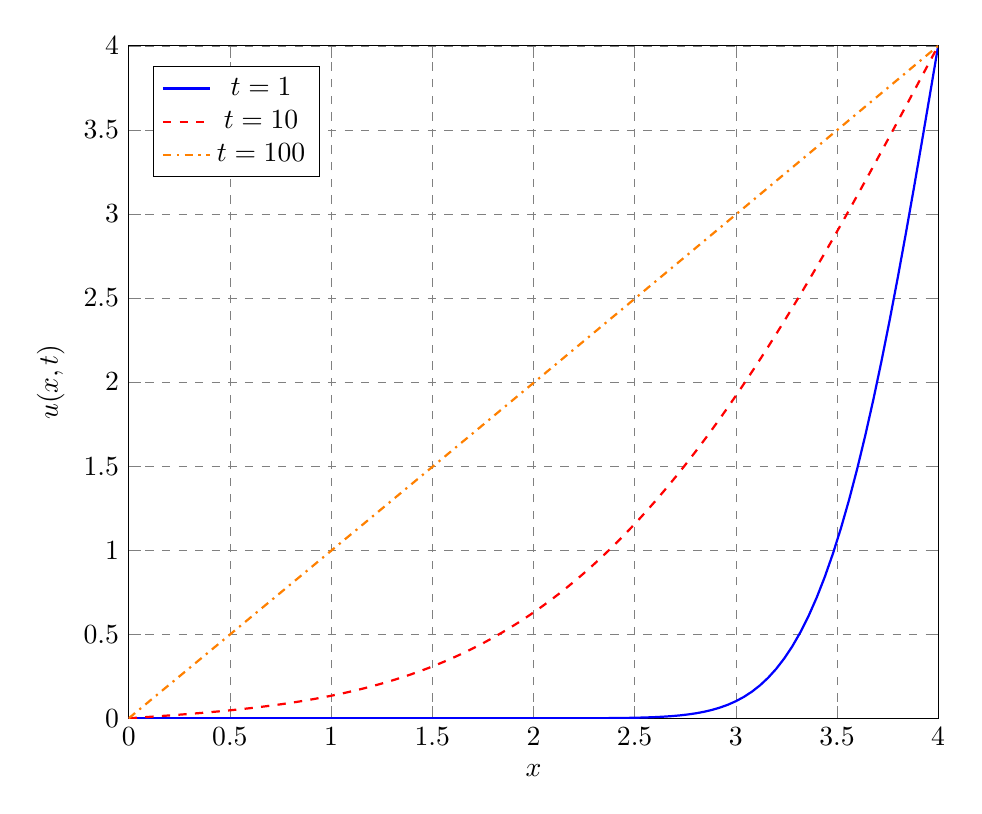
\begin{tikzpicture} \begin{axis}
[scale=1.5,
 xmin=0,  xmax=4,
 ymin=0,  ymax=4,
 grid=major, 
 major grid style={color=gray,line width=0.2pt, dashed},
 legend pos=north west,
 xlabel=$x$,
 ylabel={$u(x,t)$}
]

\addplot[line width=0.8pt, color=blue] coordinates {
 ( 0.0000e+00 , 0.0000e+00 ) 
 ( 4.0000e-02 , -2.0107e-19 ) 
 ( 8.0000e-02 , 1.5943e-17 ) 
 ( 1.2000e-01 , -1.8479e-17 ) 
 ( 1.6000e-01 , -2.1168e-17 ) 
 ( 2.0000e-01 , -5.5621e-18 ) 
 ( 2.4000e-01 , 1.1588e-16 ) 
 ( 2.8000e-01 , 4.0867e-16 ) 
 ( 3.2000e-01 , 6.6873e-16 ) 
 ( 3.6000e-01 , 1.5915e-15 ) 
 ( 4.0000e-01 , 3.4129e-15 ) 
 ( 4.4000e-01 , 6.7244e-15 ) 
 ( 4.8000e-01 , 1.3960e-14 ) 
 ( 5.2000e-01 , 2.8730e-14 ) 
 ( 5.6000e-01 , 5.7727e-14 ) 
 ( 6.0000e-01 , 1.1610e-13 ) 
 ( 6.4000e-01 , 2.3050e-13 ) 
 ( 6.8000e-01 , 4.5529e-13 ) 
 ( 7.2000e-01 , 8.9121e-13 ) 
 ( 7.6000e-01 , 1.7315e-12 ) 
 ( 8.0000e-01 , 3.3366e-12 ) 
 ( 8.4000e-01 , 6.3798e-12 ) 
 ( 8.8000e-01 , 1.2102e-11 ) 
 ( 9.2000e-01 , 2.2778e-11 ) 
 ( 9.6000e-01 , 4.2537e-11 ) 
 ( 1.0000e+00 , 7.8814e-11 ) 
 ( 1.0400e+00 , 1.4489e-10 ) 
 ( 1.0800e+00 , 2.6428e-10 ) 
 ( 1.1200e+00 , 4.7829e-10 ) 
 ( 1.1600e+00 , 8.5884e-10 ) 
 ( 1.2000e+00 , 1.5302e-09 ) 
 ( 1.2400e+00 , 2.7050e-09 ) 
 ( 1.2800e+00 , 4.7446e-09 ) 
 ( 1.3200e+00 , 8.2573e-09 ) 
 ( 1.3600e+00 , 1.4259e-08 ) 
 ( 1.4000e+00 , 2.4432e-08 ) 
 ( 1.4400e+00 , 4.1536e-08 ) 
 ( 1.4800e+00 , 7.0068e-08 ) 
 ( 1.5200e+00 , 1.1728e-07 ) 
 ( 1.5600e+00 , 1.9479e-07 ) 
 ( 1.6000e+00 , 3.2100e-07 ) 
 ( 1.6400e+00 , 5.2492e-07 ) 
 ( 1.6800e+00 , 8.5173e-07 ) 
 ( 1.7200e+00 , 1.3713e-06 ) 
 ( 1.7600e+00 , 2.1909e-06 ) 
 ( 1.8000e+00 , 3.4733e-06 ) 
 ( 1.8400e+00 , 5.4639e-06 ) 
 ( 1.8800e+00 , 8.5292e-06 ) 
 ( 1.9200e+00 , 1.3212e-05 ) 
 ( 1.9600e+00 , 2.0308e-05 ) 
 ( 2.0000e+00 , 3.0977e-05 ) 
 ( 2.0400e+00 , 4.6888e-05 ) 
 ( 2.0800e+00 , 7.0430e-05 ) 
 ( 2.1200e+00 , 1.0498e-04 ) 
 ( 2.1600e+00 , 1.5530e-04 ) 
 ( 2.2000e+00 , 2.2798e-04 ) 
 ( 2.2400e+00 , 3.3212e-04 ) 
 ( 2.2800e+00 , 4.8017e-04 ) 
 ( 2.3200e+00 , 6.8897e-04 ) 
 ( 2.3600e+00 , 9.8107e-04 ) 
 ( 2.4000e+00 , 1.3865e-03 ) 
 ( 2.4400e+00 , 1.9447e-03 ) 
 ( 2.4800e+00 , 2.7071e-03 ) 
 ( 2.5200e+00 , 3.7401e-03 ) 
 ( 2.5600e+00 , 5.1287e-03 ) 
 ( 2.6000e+00 , 6.9805e-03 ) 
 ( 2.6400e+00 , 9.4301e-03 ) 
 ( 2.6800e+00 , 1.2645e-02 ) 
 ( 2.7200e+00 , 1.6830e-02 ) 
 ( 2.7600e+00 , 2.2236e-02 ) 
 ( 2.8000e+00 , 2.9161e-02 ) 
 ( 2.8400e+00 , 3.7964e-02 ) 
 ( 2.8800e+00 , 4.9064e-02 ) 
 ( 2.9200e+00 , 6.2949e-02 ) 
 ( 2.9600e+00 , 8.0179e-02 ) 
 ( 3.0000e+00 , 1.0139e-01 ) 
 ( 3.0400e+00 , 1.2729e-01 ) 
 ( 3.0800e+00 , 1.5867e-01 ) 
 ( 3.1200e+00 , 1.9639e-01 ) 
 ( 3.1600e+00 , 2.4136e-01 ) 
 ( 3.2000e+00 , 2.9455e-01 ) 
 ( 3.2400e+00 , 3.5697e-01 ) 
 ( 3.2800e+00 , 4.2962e-01 ) 
 ( 3.3200e+00 , 5.1352e-01 ) 
 ( 3.3600e+00 , 6.0963e-01 ) 
 ( 3.4000e+00 , 7.1885e-01 ) 
 ( 3.4400e+00 , 8.4199e-01 ) 
 ( 3.4800e+00 , 9.7972e-01 ) 
 ( 3.5200e+00 , 1.1325e+00 ) 
 ( 3.5600e+00 , 1.3007e+00 ) 
 ( 3.6000e+00 , 1.4844e+00 ) 
 ( 3.6400e+00 , 1.6833e+00 ) 
 ( 3.6800e+00 , 1.8971e+00 ) 
 ( 3.7200e+00 , 2.1250e+00 ) 
 ( 3.7600e+00 , 2.3660e+00 ) 
 ( 3.8000e+00 , 2.6189e+00 ) 
 ( 3.8400e+00 , 2.8821e+00 ) 
 ( 3.8800e+00 , 3.1538e+00 ) 
 ( 3.9200e+00 , 3.4321e+00 ) 
 ( 3.9600e+00 , 3.7149e+00 ) 
 ( 4.0000e+00 , 4.0000e+00 ) 
};
\addlegendentry{$t = 1$};

\addplot[line width=0.8pt, color=red, dashed] coordinates {
 ( 0.0000e+00 , 0.0000e+00 ) 
 ( 4.0000e-02 , 3.3098e-03 ) 
 ( 8.0000e-02 , 6.6381e-03 ) 
 ( 1.2000e-01 , 1.0004e-02 ) 
 ( 1.6000e-01 , 1.3425e-02 ) 
 ( 2.0000e-01 , 1.6920e-02 ) 
 ( 2.4000e-01 , 2.0510e-02 ) 
 ( 2.8000e-01 , 2.4211e-02 ) 
 ( 3.2000e-01 , 2.8045e-02 ) 
 ( 3.6000e-01 , 3.2030e-02 ) 
 ( 4.0000e-01 , 3.6187e-02 ) 
 ( 4.4000e-01 , 4.0535e-02 ) 
 ( 4.8000e-01 , 4.5096e-02 ) 
 ( 5.2000e-01 , 4.9890e-02 ) 
 ( 5.6000e-01 , 5.4939e-02 ) 
 ( 6.0000e-01 , 6.0265e-02 ) 
 ( 6.4000e-01 , 6.5891e-02 ) 
 ( 6.8000e-01 , 7.1839e-02 ) 
 ( 7.2000e-01 , 7.8132e-02 ) 
 ( 7.6000e-01 , 8.4795e-02 ) 
 ( 8.0000e-01 , 9.1852e-02 ) 
 ( 8.4000e-01 , 9.9329e-02 ) 
 ( 8.8000e-01 , 1.0725e-01 ) 
 ( 9.2000e-01 , 1.1564e-01 ) 
 ( 9.6000e-01 , 1.2453e-01 ) 
 ( 1.0000e+00 , 1.3395e-01 ) 
 ( 1.0400e+00 , 1.4392e-01 ) 
 ( 1.0800e+00 , 1.5447e-01 ) 
 ( 1.1200e+00 , 1.6564e-01 ) 
 ( 1.1600e+00 , 1.7744e-01 ) 
 ( 1.2000e+00 , 1.8992e-01 ) 
 ( 1.2400e+00 , 2.0309e-01 ) 
 ( 1.2800e+00 , 2.1700e-01 ) 
 ( 1.3200e+00 , 2.3167e-01 ) 
 ( 1.3600e+00 , 2.4714e-01 ) 
 ( 1.4000e+00 , 2.6343e-01 ) 
 ( 1.4400e+00 , 2.8058e-01 ) 
 ( 1.4800e+00 , 2.9863e-01 ) 
 ( 1.5200e+00 , 3.1760e-01 ) 
 ( 1.5600e+00 , 3.3753e-01 ) 
 ( 1.6000e+00 , 3.5844e-01 ) 
 ( 1.6400e+00 , 3.8038e-01 ) 
 ( 1.6800e+00 , 4.0338e-01 ) 
 ( 1.7200e+00 , 4.2746e-01 ) 
 ( 1.7600e+00 , 4.5266e-01 ) 
 ( 1.8000e+00 , 4.7902e-01 ) 
 ( 1.8400e+00 , 5.0655e-01 ) 
 ( 1.8800e+00 , 5.3530e-01 ) 
 ( 1.9200e+00 , 5.6529e-01 ) 
 ( 1.9600e+00 , 5.9655e-01 ) 
 ( 2.0000e+00 , 6.2911e-01 ) 
 ( 2.0400e+00 , 6.6300e-01 ) 
 ( 2.0800e+00 , 6.9824e-01 ) 
 ( 2.1200e+00 , 7.3486e-01 ) 
 ( 2.1600e+00 , 7.7288e-01 ) 
 ( 2.2000e+00 , 8.1232e-01 ) 
 ( 2.2400e+00 , 8.5321e-01 ) 
 ( 2.2800e+00 , 8.9556e-01 ) 
 ( 2.3200e+00 , 9.3940e-01 ) 
 ( 2.3600e+00 , 9.8473e-01 ) 
 ( 2.4000e+00 , 1.0316e+00 ) 
 ( 2.4400e+00 , 1.0799e+00 ) 
 ( 2.4800e+00 , 1.1298e+00 ) 
 ( 2.5200e+00 , 1.1813e+00 ) 
 ( 2.5600e+00 , 1.2343e+00 ) 
 ( 2.6000e+00 , 1.2888e+00 ) 
 ( 2.6400e+00 , 1.3449e+00 ) 
 ( 2.6800e+00 , 1.4025e+00 ) 
 ( 2.7200e+00 , 1.4616e+00 ) 
 ( 2.7600e+00 , 1.5223e+00 ) 
 ( 2.8000e+00 , 1.5846e+00 ) 
 ( 2.8400e+00 , 1.6483e+00 ) 
 ( 2.8800e+00 , 1.7135e+00 ) 
 ( 2.9200e+00 , 1.7802e+00 ) 
 ( 2.9600e+00 , 1.8484e+00 ) 
 ( 3.0000e+00 , 1.9180e+00 ) 
 ( 3.0400e+00 , 1.9890e+00 ) 
 ( 3.0800e+00 , 2.0614e+00 ) 
 ( 3.1200e+00 , 2.1351e+00 ) 
 ( 3.1600e+00 , 2.2101e+00 ) 
 ( 3.2000e+00 , 2.2864e+00 ) 
 ( 3.2400e+00 , 2.3640e+00 ) 
 ( 3.2800e+00 , 2.4427e+00 ) 
 ( 3.3200e+00 , 2.5225e+00 ) 
 ( 3.3600e+00 , 2.6035e+00 ) 
 ( 3.4000e+00 , 2.6855e+00 ) 
 ( 3.4400e+00 , 2.7685e+00 ) 
 ( 3.4800e+00 , 2.8524e+00 ) 
 ( 3.5200e+00 , 2.9372e+00 ) 
 ( 3.5600e+00 , 3.0228e+00 ) 
 ( 3.6000e+00 , 3.1092e+00 ) 
 ( 3.6400e+00 , 3.1963e+00 ) 
 ( 3.6800e+00 , 3.2840e+00 ) 
 ( 3.7200e+00 , 3.3722e+00 ) 
 ( 3.7600e+00 , 3.4610e+00 ) 
 ( 3.8000e+00 , 3.5501e+00 ) 
 ( 3.8400e+00 , 3.6397e+00 ) 
 ( 3.8800e+00 , 3.7295e+00 ) 
 ( 3.9200e+00 , 3.8196e+00 ) 
 ( 3.9600e+00 , 3.9097e+00 ) 
 ( 4.0000e+00 , 4.0000e+00 ) 
};
\addlegendentry{$t = 10$};

\addplot[line width=0.8pt, color=orange, dash dot] coordinates {
 ( 0.0000e+00 , 0.0000e+00 ) 
 ( 4.0000e-02 , 3.9832e-02 ) 
 ( 8.0000e-02 , 7.9665e-02 ) 
 ( 1.2000e-01 , 1.1950e-01 ) 
 ( 1.6000e-01 , 1.5933e-01 ) 
 ( 2.0000e-01 , 1.9917e-01 ) 
 ( 2.4000e-01 , 2.3900e-01 ) 
 ( 2.8000e-01 , 2.7884e-01 ) 
 ( 3.2000e-01 , 3.1867e-01 ) 
 ( 3.6000e-01 , 3.5851e-01 ) 
 ( 4.0000e-01 , 3.9835e-01 ) 
 ( 4.4000e-01 , 4.3819e-01 ) 
 ( 4.8000e-01 , 4.7804e-01 ) 
 ( 5.2000e-01 , 5.1788e-01 ) 
 ( 5.6000e-01 , 5.5773e-01 ) 
 ( 6.0000e-01 , 5.9758e-01 ) 
 ( 6.4000e-01 , 6.3743e-01 ) 
 ( 6.8000e-01 , 6.7729e-01 ) 
 ( 7.2000e-01 , 7.1714e-01 ) 
 ( 7.6000e-01 , 7.5700e-01 ) 
 ( 8.0000e-01 , 7.9687e-01 ) 
 ( 8.4000e-01 , 8.3673e-01 ) 
 ( 8.8000e-01 , 8.7660e-01 ) 
 ( 9.2000e-01 , 9.1647e-01 ) 
 ( 9.6000e-01 , 9.5635e-01 ) 
 ( 1.0000e+00 , 9.9623e-01 ) 
 ( 1.0400e+00 , 1.0361e+00 ) 
 ( 1.0800e+00 , 1.0760e+00 ) 
 ( 1.1200e+00 , 1.1159e+00 ) 
 ( 1.1600e+00 , 1.1558e+00 ) 
 ( 1.2000e+00 , 1.1957e+00 ) 
 ( 1.2400e+00 , 1.2356e+00 ) 
 ( 1.2800e+00 , 1.2755e+00 ) 
 ( 1.3200e+00 , 1.3154e+00 ) 
 ( 1.3600e+00 , 1.3553e+00 ) 
 ( 1.4000e+00 , 1.3952e+00 ) 
 ( 1.4400e+00 , 1.4352e+00 ) 
 ( 1.4800e+00 , 1.4751e+00 ) 
 ( 1.5200e+00 , 1.5150e+00 ) 
 ( 1.5600e+00 , 1.5550e+00 ) 
 ( 1.6000e+00 , 1.5949e+00 ) 
 ( 1.6400e+00 , 1.6349e+00 ) 
 ( 1.6800e+00 , 1.6748e+00 ) 
 ( 1.7200e+00 , 1.7148e+00 ) 
 ( 1.7600e+00 , 1.7548e+00 ) 
 ( 1.8000e+00 , 1.7947e+00 ) 
 ( 1.8400e+00 , 1.8347e+00 ) 
 ( 1.8800e+00 , 1.8747e+00 ) 
 ( 1.9200e+00 , 1.9147e+00 ) 
 ( 1.9600e+00 , 1.9547e+00 ) 
 ( 2.0000e+00 , 1.9947e+00 ) 
 ( 2.0400e+00 , 2.0347e+00 ) 
 ( 2.0800e+00 , 2.0747e+00 ) 
 ( 2.1200e+00 , 2.1147e+00 ) 
 ( 2.1600e+00 , 2.1547e+00 ) 
 ( 2.2000e+00 , 2.1947e+00 ) 
 ( 2.2400e+00 , 2.2348e+00 ) 
 ( 2.2800e+00 , 2.2748e+00 ) 
 ( 2.3200e+00 , 2.3148e+00 ) 
 ( 2.3600e+00 , 2.3549e+00 ) 
 ( 2.4000e+00 , 2.3949e+00 ) 
 ( 2.4400e+00 , 2.4350e+00 ) 
 ( 2.4800e+00 , 2.4750e+00 ) 
 ( 2.5200e+00 , 2.5151e+00 ) 
 ( 2.5600e+00 , 2.5552e+00 ) 
 ( 2.6000e+00 , 2.5952e+00 ) 
 ( 2.6400e+00 , 2.6353e+00 ) 
 ( 2.6800e+00 , 2.6754e+00 ) 
 ( 2.7200e+00 , 2.7155e+00 ) 
 ( 2.7600e+00 , 2.7556e+00 ) 
 ( 2.8000e+00 , 2.7957e+00 ) 
 ( 2.8400e+00 , 2.8358e+00 ) 
 ( 2.8800e+00 , 2.8759e+00 ) 
 ( 2.9200e+00 , 2.9160e+00 ) 
 ( 2.9600e+00 , 2.9561e+00 ) 
 ( 3.0000e+00 , 2.9962e+00 ) 
 ( 3.0400e+00 , 3.0363e+00 ) 
 ( 3.0800e+00 , 3.0765e+00 ) 
 ( 3.1200e+00 , 3.1166e+00 ) 
 ( 3.1600e+00 , 3.1567e+00 ) 
 ( 3.2000e+00 , 3.1969e+00 ) 
 ( 3.2400e+00 , 3.2370e+00 ) 
 ( 3.2800e+00 , 3.2771e+00 ) 
 ( 3.3200e+00 , 3.3173e+00 ) 
 ( 3.3600e+00 , 3.3574e+00 ) 
 ( 3.4000e+00 , 3.3976e+00 ) 
 ( 3.4400e+00 , 3.4377e+00 ) 
 ( 3.4800e+00 , 3.4779e+00 ) 
 ( 3.5200e+00 , 3.5180e+00 ) 
 ( 3.5600e+00 , 3.5582e+00 ) 
 ( 3.6000e+00 , 3.5984e+00 ) 
 ( 3.6400e+00 , 3.6385e+00 ) 
 ( 3.6800e+00 , 3.6787e+00 ) 
 ( 3.7200e+00 , 3.7188e+00 ) 
 ( 3.7600e+00 , 3.7590e+00 ) 
 ( 3.8000e+00 , 3.7992e+00 ) 
 ( 3.8400e+00 , 3.8393e+00 ) 
 ( 3.8800e+00 , 3.8795e+00 ) 
 ( 3.9200e+00 , 3.9197e+00 ) 
 ( 3.9600e+00 , 3.9598e+00 ) 
 ( 4.0000e+00 , 4.0000e+00 )
};
\addlegendentry{$t = 100$};

\end{axis}
\end{tikzpicture}

\caption{Plot of transient heat conduction for the case with different temperatures specified at the domain boundaries.}
\label{Fig:pde_transientHeatCondution_Asymmetric_Example}
\end{center}
\end{figure}

Let us now try an example where the initial condition satisfies $f(x,0) = 0$, a flat temperature, with $L = 4$ and $\alpha = 0.1$. Instantaneously at $t = 0$, the temperature of the right boundary is brought to $u_r = 4$. From inserting numbers, we know that the steady-state solution will be a straight line with $u = 0$ and $x = 0$ and $u = 4$ at $x = 4$.

A few snapshots of the solution in time are shown in Fig.~\ref{Fig:pde_transientHeatCondution_Asymmetric_Example}. At $t = 1$, the thermal energy begins to diffuse into the medium and raise the temperature near the right-boundary. The left boundary is largely unaffected, as there has not yet been sufficient time for the thermal energy to propagate through the entire domain. At $t = 10$, the thermal energy has reached the left boundary, but the shape of the temperature field still has curvature as the temperature has not yet equilibrated. By $t = 100$, the system has almost reached its equilibrium state where the temperature field is given by a straight line connecting the two boundaries.

%%%%%%%%%%%%%%%%%%%%%%%%%%%%%%%%%%%%%%%%%%%%%%%%%%%%%%%%%%%%%%%%%%%%%%%%%%%%%%%%%%%%%%%%%%%%%%%
\subsection{Example: Transient Heat Conduction with Constant Source}

The superposition principle also allows us to solve cases where we have an inhomogeneous term. Consider the problem
\begin{align}
  \dho{u}{t} - \alpha \dhotwo{u}{x} = Q, \quad u(x,0) = f(x), \quad u(0,t) = u(L,t) = 0 .
\end{align}
Here $Q$ represents a constant heat generation rate. As before, we apply superposition and write the solution as a transient plus steady-state solution:
\begin{align}
  u(x,t) = v(x,t) + s(x) . \nonumber
\end{align}
Inserting the steady state solution into the differential equation gives the ordinary differential equation
\begin{align}
  -\alpha \frac{d^2 s}{dx^2} = Q,  \quad u(0,t) = u(L,t) = 0 .
\end{align}
Solving this and applying the boundary conditions yields the steady-state solution
\begin{align}
  s(x) = \frac{ Q }{ 2 \alpha } x ( L - x ).
\end{align}

Now we insert the expanded form of $u(x,t)$ into the original differential equation
\begin{align}
  \dho{v}{t} - \alpha \dhotwo{v}{x} - \alpha \dhotwo{}{x} \left[ \frac{ Q }{ 2 \alpha } x ( L - x ) \right] = Q .
\end{align}
Since
\begin{align}
  - \alpha \dhotwo{}{x} \left[ \frac{ Q }{ 2 \alpha } x ( L - x ) \right] = Q \nonumber
\end{align}
this will cancel out the inhomogeneous term to yield a homogeneous problem. We perform the same analysis as with the case with asymmetric boundary conditions to fully describe the problem for the transient part
\begin{align}
  \dho{v}{t} - \alpha \dhotwo{v}{x} = 0 , \quad v(x,0) = f(x) - s(x), \quad v(0,t) = 0, \quad v(L,t) = 0 ,
\end{align}
which is identical to the previous problem except that $s(x)$ has a different form. The solution to the transient problem is
\begin{align}
  v(x,t) &= \sum_{n=1}^\infty A_n \sin \left( \frac{ n \pi x }{ L } \right)  \exp \left[ -\alpha \left( \frac{ n \pi }{ L } \right)^2 t \right] .
\end{align}
Adding on the steady-state solution gives the full solution
\begin{align}
  u(x,t) &= \frac{ Q }{ 2 \alpha } x ( L - x ) + \sum_{n=1}^\infty A_n \sin \left( \frac{ n \pi x }{ L } \right)  \exp \left[ -\alpha \left( \frac{ n \pi }{ L } \right)^2 t \right] 
\end{align}
where the coefficients are
\begin{align}
  A_n &=  \frac{2}{L} \int_0^L \sin \left( \frac{ n \pi x }{ L } \right) \left( f(x) - \frac{ Q }{ 2 \alpha } x ( L - x ) \right) dx  \nonumber \\
      &= \frac{2 Q L^2 }{ \alpha n^3 \pi^3 } \left[ (-1)^n - 1 \right] + \frac{2}{L} \int_0^L \sin \left( \frac{ n \pi x }{ L } \right) f(x) dx .
\end{align}

\begin{figure}[b!]
\begin{center}
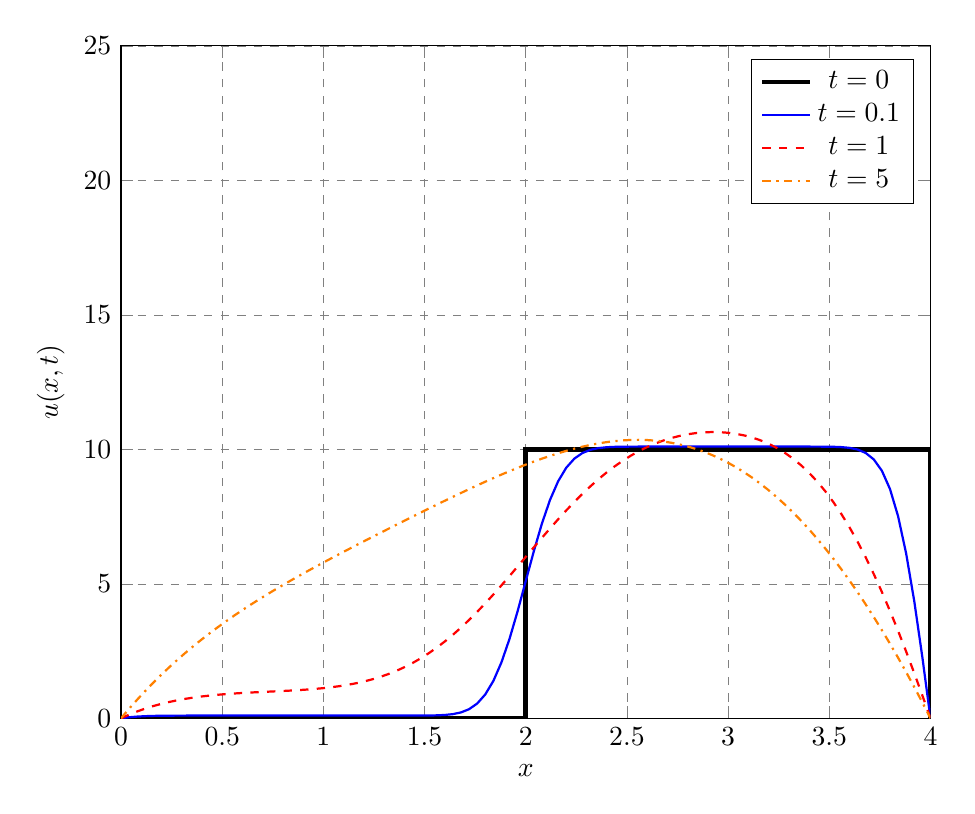
\begin{tikzpicture} \begin{axis}
[scale=1.5,
 xmin=0,  xmax=4,
 ymin=0,  ymax=25,
 grid=major, 
 major grid style={color=gray,line width=0.2pt, dashed},
 xlabel=$x$,
 ylabel={$u(x,t)$}
]

\addplot[line width=0.6mm, color=black] coordinates {
(  0 , 0 )
(  2 , 0 )
(  2 , 10 )
(  4 , 10 )
(  4 , 0 )
};
\addlegendentry{$t = 0$};

\addplot[line width=0.8pt, color=blue] coordinates {
 ( 0.0000e+00 , 0.0000e+00 ) 
 ( 4.0000e-02 , 3.7735e-02 ) 
 ( 8.0000e-02 , 6.3009e-02 ) 
 ( 1.2000e-01 , 7.9098e-02 ) 
 ( 1.6000e-01 , 8.8798e-02 ) 
 ( 2.0000e-01 , 9.4321e-02 ) 
 ( 2.4000e-01 , 9.7283e-02 ) 
 ( 2.8000e-01 , 9.8776e-02 ) 
 ( 3.2000e-01 , 9.9482e-02 ) 
 ( 3.6000e-01 , 9.9794e-02 ) 
 ( 4.0000e-01 , 9.9923e-02 ) 
 ( 4.4000e-01 , 9.9973e-02 ) 
 ( 4.8000e-01 , 9.9991e-02 ) 
 ( 5.2000e-01 , 9.9997e-02 ) 
 ( 5.6000e-01 , 9.9999e-02 ) 
 ( 6.0000e-01 , 1.0000e-01 ) 
 ( 6.4000e-01 , 1.0000e-01 ) 
 ( 6.8000e-01 , 1.0000e-01 ) 
 ( 7.2000e-01 , 1.0000e-01 ) 
 ( 7.6000e-01 , 1.0000e-01 ) 
 ( 8.0000e-01 , 1.0000e-01 ) 
 ( 8.4000e-01 , 1.0000e-01 ) 
 ( 8.8000e-01 , 1.0000e-01 ) 
 ( 9.2000e-01 , 1.0000e-01 ) 
 ( 9.6000e-01 , 1.0000e-01 ) 
 ( 1.0000e+00 , 1.0000e-01 ) 
 ( 1.0400e+00 , 1.0000e-01 ) 
 ( 1.0800e+00 , 1.0000e-01 ) 
 ( 1.1200e+00 , 1.0000e-01 ) 
 ( 1.1600e+00 , 1.0000e-01 ) 
 ( 1.2000e+00 , 1.0000e-01 ) 
 ( 1.2400e+00 , 1.0000e-01 ) 
 ( 1.2800e+00 , 1.0000e-01 ) 
 ( 1.3200e+00 , 1.0001e-01 ) 
 ( 1.3600e+00 , 1.0003e-01 ) 
 ( 1.4000e+00 , 1.0011e-01 ) 
 ( 1.4400e+00 , 1.0038e-01 ) 
 ( 1.4800e+00 , 1.0118e-01 ) 
 ( 1.5200e+00 , 1.0344e-01 ) 
 ( 1.5600e+00 , 1.0931e-01 ) 
 ( 1.6000e+00 , 1.2339e-01 ) 
 ( 1.6400e+00 , 1.5455e-01 ) 
 ( 1.6800e+00 , 2.1826e-01 ) 
 ( 1.7200e+00 , 3.3857e-01 ) 
 ( 1.7600e+00 , 5.4843e-01 ) 
 ( 1.8000e+00 , 8.8650e-01 ) 
 ( 1.8400e+00 , 1.3895e+00 ) 
 ( 1.8800e+00 , 2.0807e+00 ) 
 ( 1.9200e+00 , 2.9580e+00 ) 
 ( 1.9600e+00 , 3.9865e+00 ) 
 ( 2.0000e+00 , 5.1000e+00 ) 
 ( 2.0400e+00 , 6.2135e+00 ) 
 ( 2.0800e+00 , 7.2420e+00 ) 
 ( 2.1200e+00 , 8.1193e+00 ) 
 ( 2.1600e+00 , 8.8105e+00 ) 
 ( 2.2000e+00 , 9.3135e+00 ) 
 ( 2.2400e+00 , 9.6516e+00 ) 
 ( 2.2800e+00 , 9.8614e+00 ) 
 ( 2.3200e+00 , 9.9817e+00 ) 
 ( 2.3600e+00 , 1.0045e+01 ) 
 ( 2.4000e+00 , 1.0077e+01 ) 
 ( 2.4400e+00 , 1.0091e+01 ) 
 ( 2.4800e+00 , 1.0097e+01 ) 
 ( 2.5200e+00 , 1.0099e+01 ) 
 ( 2.5600e+00 , 1.0100e+01 ) 
 ( 2.6000e+00 , 1.0100e+01 ) 
 ( 2.6400e+00 , 1.0100e+01 ) 
 ( 2.6800e+00 , 1.0100e+01 ) 
 ( 2.7200e+00 , 1.0100e+01 ) 
 ( 2.7600e+00 , 1.0100e+01 ) 
 ( 2.8000e+00 , 1.0100e+01 ) 
 ( 2.8400e+00 , 1.0100e+01 ) 
 ( 2.8800e+00 , 1.0100e+01 ) 
 ( 2.9200e+00 , 1.0100e+01 ) 
 ( 2.9600e+00 , 1.0100e+01 ) 
 ( 3.0000e+00 , 1.0100e+01 ) 
 ( 3.0400e+00 , 1.0100e+01 ) 
 ( 3.0800e+00 , 1.0100e+01 ) 
 ( 3.1200e+00 , 1.0100e+01 ) 
 ( 3.1600e+00 , 1.0100e+01 ) 
 ( 3.2000e+00 , 1.0100e+01 ) 
 ( 3.2400e+00 , 1.0100e+01 ) 
 ( 3.2800e+00 , 1.0100e+01 ) 
 ( 3.3200e+00 , 1.0100e+01 ) 
 ( 3.3600e+00 , 1.0100e+01 ) 
 ( 3.4000e+00 , 1.0100e+01 ) 
 ( 3.4400e+00 , 1.0099e+01 ) 
 ( 3.4800e+00 , 1.0098e+01 ) 
 ( 3.5200e+00 , 1.0093e+01 ) 
 ( 3.5600e+00 , 1.0081e+01 ) 
 ( 3.6000e+00 , 1.0053e+01 ) 
 ( 3.6400e+00 , 9.9907e+00 ) 
 ( 3.6800e+00 , 9.8630e+00 ) 
 ( 3.7200e+00 , 9.6216e+00 ) 
 ( 3.7600e+00 , 9.2004e+00 ) 
 ( 3.8000e+00 , 8.5213e+00 ) 
 ( 3.8400e+00 , 7.5098e+00 ) 
 ( 3.8800e+00 , 6.1177e+00 ) 
 ( 3.9200e+00 , 4.3469e+00 ) 
 ( 3.9600e+00 , 2.2648e+00 ) 
 ( 4.0000e+00 , 6.5967e-15 ) 
};
\addlegendentry{$t = 0.1$};

\addplot[line width=0.8pt, color=red, dashed] coordinates {
 ( 0.0000e+00 , 0.0000e+00 ) 
 ( 4.0000e-02 , 1.3495e-01 ) 
 ( 8.0000e-02 , 2.5505e-01 ) 
 ( 1.2000e-01 , 3.6143e-01 ) 
 ( 1.6000e-01 , 4.5521e-01 ) 
 ( 2.0000e-01 , 5.3748e-01 ) 
 ( 2.4000e-01 , 6.0932e-01 ) 
 ( 2.8000e-01 , 6.7174e-01 ) 
 ( 3.2000e-01 , 7.2573e-01 ) 
 ( 3.6000e-01 , 7.7223e-01 ) 
 ( 4.0000e-01 , 8.1214e-01 ) 
 ( 4.4000e-01 , 8.4629e-01 ) 
 ( 4.8000e-01 , 8.7549e-01 ) 
 ( 5.2000e-01 , 9.0050e-01 ) 
 ( 5.6000e-01 , 9.2202e-01 ) 
 ( 6.0000e-01 , 9.4075e-01 ) 
 ( 6.4000e-01 , 9.5735e-01 ) 
 ( 6.8000e-01 , 9.7246e-01 ) 
 ( 7.2000e-01 , 9.8673e-01 ) 
 ( 7.6000e-01 , 1.0008e+00 ) 
 ( 8.0000e-01 , 1.0153e+00 ) 
 ( 8.4000e-01 , 1.0310e+00 ) 
 ( 8.8000e-01 , 1.0486e+00 ) 
 ( 9.2000e-01 , 1.0689e+00 ) 
 ( 9.6000e-01 , 1.0928e+00 ) 
 ( 1.0000e+00 , 1.1211e+00 ) 
 ( 1.0400e+00 , 1.1549e+00 ) 
 ( 1.0800e+00 , 1.1952e+00 ) 
 ( 1.1200e+00 , 1.2431e+00 ) 
 ( 1.1600e+00 , 1.3000e+00 ) 
 ( 1.2000e+00 , 1.3669e+00 ) 
 ( 1.2400e+00 , 1.4453e+00 ) 
 ( 1.2800e+00 , 1.5363e+00 ) 
 ( 1.3200e+00 , 1.6414e+00 ) 
 ( 1.3600e+00 , 1.7617e+00 ) 
 ( 1.4000e+00 , 1.8983e+00 ) 
 ( 1.4400e+00 , 2.0523e+00 ) 
 ( 1.4800e+00 , 2.2245e+00 ) 
 ( 1.5200e+00 , 2.4156e+00 ) 
 ( 1.5600e+00 , 2.6258e+00 ) 
 ( 1.6000e+00 , 2.8554e+00 ) 
 ( 1.6400e+00 , 3.1041e+00 ) 
 ( 1.6800e+00 , 3.3714e+00 ) 
 ( 1.7200e+00 , 3.6562e+00 ) 
 ( 1.7600e+00 , 3.9575e+00 ) 
 ( 1.8000e+00 , 4.2736e+00 ) 
 ( 1.8400e+00 , 4.6026e+00 ) 
 ( 1.8800e+00 , 4.9422e+00 ) 
 ( 1.9200e+00 , 5.2901e+00 ) 
 ( 1.9600e+00 , 5.6436e+00 ) 
 ( 2.0000e+00 , 5.9999e+00 ) 
 ( 2.0400e+00 , 6.3562e+00 ) 
 ( 2.0800e+00 , 6.7097e+00 ) 
 ( 2.1200e+00 , 7.0575e+00 ) 
 ( 2.1600e+00 , 7.3970e+00 ) 
 ( 2.2000e+00 , 7.7258e+00 ) 
 ( 2.2400e+00 , 8.0416e+00 ) 
 ( 2.2800e+00 , 8.3425e+00 ) 
 ( 2.3200e+00 , 8.6269e+00 ) 
 ( 2.3600e+00 , 8.8934e+00 ) 
 ( 2.4000e+00 , 9.1410e+00 ) 
 ( 2.4400e+00 , 9.3692e+00 ) 
 ( 2.4800e+00 , 9.5775e+00 ) 
 ( 2.5200e+00 , 9.7659e+00 ) 
 ( 2.5600e+00 , 9.9345e+00 ) 
 ( 2.6000e+00 , 1.0084e+01 ) 
 ( 2.6400e+00 , 1.0214e+01 ) 
 ( 2.6800e+00 , 1.0326e+01 ) 
 ( 2.7200e+00 , 1.0420e+01 ) 
 ( 2.7600e+00 , 1.0497e+01 ) 
 ( 2.8000e+00 , 1.0558e+01 ) 
 ( 2.8400e+00 , 1.0602e+01 ) 
 ( 2.8800e+00 , 1.0629e+01 ) 
 ( 2.9200e+00 , 1.0641e+01 ) 
 ( 2.9600e+00 , 1.0636e+01 ) 
 ( 3.0000e+00 , 1.0614e+01 ) 
 ( 3.0400e+00 , 1.0574e+01 ) 
 ( 3.0800e+00 , 1.0515e+01 ) 
 ( 3.1200e+00 , 1.0435e+01 ) 
 ( 3.1600e+00 , 1.0333e+01 ) 
 ( 3.2000e+00 , 1.0206e+01 ) 
 ( 3.2400e+00 , 1.0053e+01 ) 
 ( 3.2800e+00 , 9.8706e+00 ) 
 ( 3.3200e+00 , 9.6571e+00 ) 
 ( 3.3600e+00 , 9.4097e+00 ) 
 ( 3.4000e+00 , 9.1262e+00 ) 
 ( 3.4400e+00 , 8.8042e+00 ) 
 ( 3.4800e+00 , 8.4419e+00 ) 
 ( 3.5200e+00 , 8.0374e+00 ) 
 ( 3.5600e+00 , 7.5896e+00 ) 
 ( 3.6000e+00 , 7.0977e+00 ) 
 ( 3.6400e+00 , 6.5615e+00 ) 
 ( 3.6800e+00 , 5.9813e+00 ) 
 ( 3.7200e+00 , 5.3580e+00 ) 
 ( 3.7600e+00 , 4.6934e+00 ) 
 ( 3.8000e+00 , 3.9897e+00 ) 
 ( 3.8400e+00 , 3.2497e+00 ) 
 ( 3.8800e+00 , 2.4767e+00 ) 
 ( 3.9200e+00 , 1.6746e+00 ) 
 ( 3.9600e+00 , 8.4759e-01 ) 
 ( 4.0000e+00 , 2.2075e-16 )
};
\addlegendentry{$t = 1$};

\addplot[line width=0.8pt, color=orange, dash dot] coordinates {
 ( 0.0000e+00 , 0.0000e+00 ) 
 ( 4.0000e-02 , 3.5424e-01 ) 
 ( 8.0000e-02 , 6.9319e-01 ) 
 ( 1.2000e-01 , 1.0176e+00 ) 
 ( 1.6000e-01 , 1.3281e+00 ) 
 ( 2.0000e-01 , 1.6254e+00 ) 
 ( 2.4000e-01 , 1.9103e+00 ) 
 ( 2.8000e-01 , 2.1834e+00 ) 
 ( 3.2000e-01 , 2.4454e+00 ) 
 ( 3.6000e-01 , 2.6969e+00 ) 
 ( 4.0000e-01 , 2.9387e+00 ) 
 ( 4.4000e-01 , 3.1714e+00 ) 
 ( 4.8000e-01 , 3.3956e+00 ) 
 ( 5.2000e-01 , 3.6119e+00 ) 
 ( 5.6000e-01 , 3.8210e+00 ) 
 ( 6.0000e-01 , 4.0233e+00 ) 
 ( 6.4000e-01 , 4.2196e+00 ) 
 ( 6.8000e-01 , 4.4102e+00 ) 
 ( 7.2000e-01 , 4.5958e+00 ) 
 ( 7.6000e-01 , 4.7767e+00 ) 
 ( 8.0000e-01 , 4.9536e+00 ) 
 ( 8.4000e-01 , 5.1268e+00 ) 
 ( 8.8000e-01 , 5.2967e+00 ) 
 ( 9.2000e-01 , 5.4637e+00 ) 
 ( 9.6000e-01 , 5.6283e+00 ) 
 ( 1.0000e+00 , 5.7906e+00 ) 
 ( 1.0400e+00 , 5.9511e+00 ) 
 ( 1.0800e+00 , 6.1099e+00 ) 
 ( 1.1200e+00 , 6.2674e+00 ) 
 ( 1.1600e+00 , 6.4236e+00 ) 
 ( 1.2000e+00 , 6.5789e+00 ) 
 ( 1.2400e+00 , 6.7332e+00 ) 
 ( 1.2800e+00 , 6.8868e+00 ) 
 ( 1.3200e+00 , 7.0396e+00 ) 
 ( 1.3600e+00 , 7.1918e+00 ) 
 ( 1.4000e+00 , 7.3432e+00 ) 
 ( 1.4400e+00 , 7.4939e+00 ) 
 ( 1.4800e+00 , 7.6438e+00 ) 
 ( 1.5200e+00 , 7.7928e+00 ) 
 ( 1.5600e+00 , 7.9408e+00 ) 
 ( 1.6000e+00 , 8.0875e+00 ) 
 ( 1.6400e+00 , 8.2328e+00 ) 
 ( 1.6800e+00 , 8.3765e+00 ) 
 ( 1.7200e+00 , 8.5183e+00 ) 
 ( 1.7600e+00 , 8.6578e+00 ) 
 ( 1.8000e+00 , 8.7949e+00 ) 
 ( 1.8400e+00 , 8.9291e+00 ) 
 ( 1.8800e+00 , 9.0601e+00 ) 
 ( 1.9200e+00 , 9.1874e+00 ) 
 ( 1.9600e+00 , 9.3108e+00 ) 
 ( 2.0000e+00 , 9.4296e+00 ) 
 ( 2.0400e+00 , 9.5436e+00 ) 
 ( 2.0800e+00 , 9.6522e+00 ) 
 ( 2.1200e+00 , 9.7549e+00 ) 
 ( 2.1600e+00 , 9.8512e+00 ) 
 ( 2.2000e+00 , 9.9407e+00 ) 
 ( 2.2400e+00 , 1.0023e+01 ) 
 ( 2.2800e+00 , 1.0097e+01 ) 
 ( 2.3200e+00 , 1.0163e+01 ) 
 ( 2.3600e+00 , 1.0220e+01 ) 
 ( 2.4000e+00 , 1.0267e+01 ) 
 ( 2.4400e+00 , 1.0304e+01 ) 
 ( 2.4800e+00 , 1.0331e+01 ) 
 ( 2.5200e+00 , 1.0347e+01 ) 
 ( 2.5600e+00 , 1.0351e+01 ) 
 ( 2.6000e+00 , 1.0343e+01 ) 
 ( 2.6400e+00 , 1.0322e+01 ) 
 ( 2.6800e+00 , 1.0289e+01 ) 
 ( 2.7200e+00 , 1.0242e+01 ) 
 ( 2.7600e+00 , 1.0181e+01 ) 
 ( 2.8000e+00 , 1.0105e+01 ) 
 ( 2.8400e+00 , 1.0015e+01 ) 
 ( 2.8800e+00 , 9.9095e+00 ) 
 ( 2.9200e+00 , 9.7885e+00 ) 
 ( 2.9600e+00 , 9.6516e+00 ) 
 ( 3.0000e+00 , 9.4984e+00 ) 
 ( 3.0400e+00 , 9.3287e+00 ) 
 ( 3.0800e+00 , 9.1423e+00 ) 
 ( 3.1200e+00 , 8.9388e+00 ) 
 ( 3.1600e+00 , 8.7181e+00 ) 
 ( 3.2000e+00 , 8.4799e+00 ) 
 ( 3.2400e+00 , 8.2242e+00 ) 
 ( 3.2800e+00 , 7.9507e+00 ) 
 ( 3.3200e+00 , 7.6594e+00 ) 
 ( 3.3600e+00 , 7.3502e+00 ) 
 ( 3.4000e+00 , 7.0231e+00 ) 
 ( 3.4400e+00 , 6.6780e+00 ) 
 ( 3.4800e+00 , 6.3149e+00 ) 
 ( 3.5200e+00 , 5.9339e+00 ) 
 ( 3.5600e+00 , 5.5349e+00 ) 
 ( 3.6000e+00 , 5.1182e+00 ) 
 ( 3.6400e+00 , 4.6838e+00 ) 
 ( 3.6800e+00 , 4.2317e+00 ) 
 ( 3.7200e+00 , 3.7622e+00 ) 
 ( 3.7600e+00 , 3.2753e+00 ) 
 ( 3.8000e+00 , 2.7712e+00 ) 
 ( 3.8400e+00 , 2.2502e+00 ) 
 ( 3.8800e+00 , 1.7124e+00 ) 
 ( 3.9200e+00 , 1.1579e+00 ) 
 ( 3.9600e+00 , 5.8707e-01 ) 
 ( 4.0000e+00 , -7.9872e-16 ) 
};
\addlegendentry{$t = 5$};

\end{axis}
\end{tikzpicture}

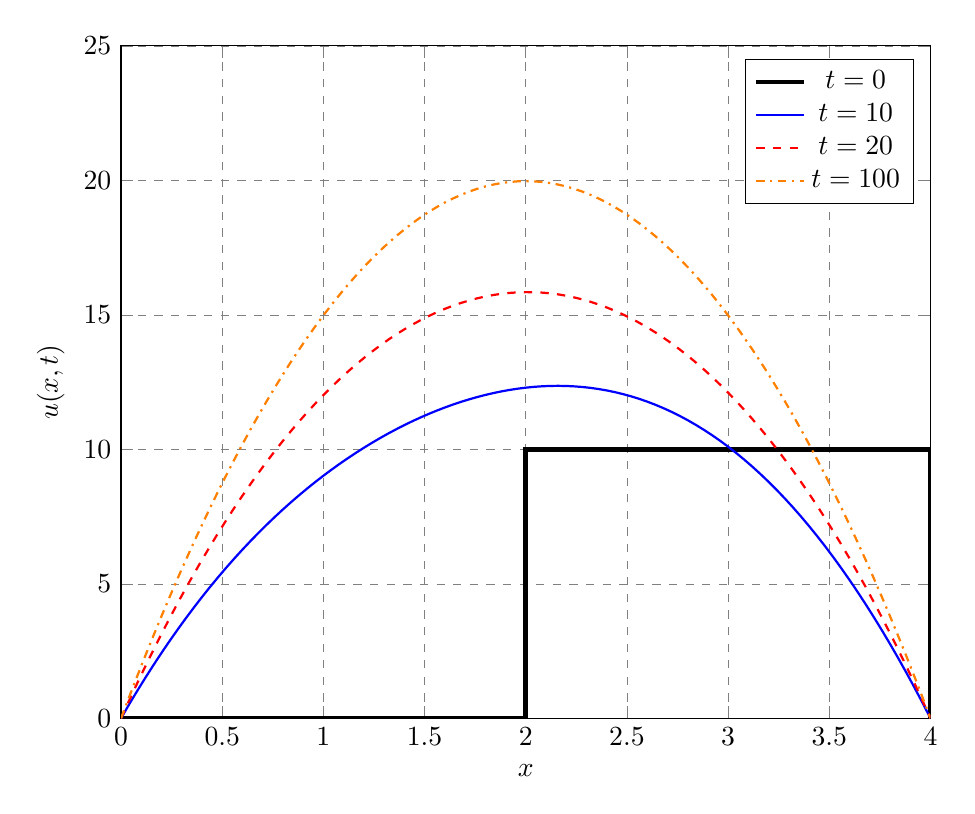
\begin{tikzpicture} \begin{axis}
[scale=1.5,
 xmin=0,  xmax=4,
 ymin=0,  ymax=25,
 grid=major, 
 major grid style={color=gray,line width=0.2pt, dashed},
 xlabel=$x$,
 ylabel={$u(x,t)$}
]

\addplot[line width=0.6mm, color=black] coordinates {
(  0 , 0 )
(  2 , 0 )
(  2 , 10 )
(  4 , 10 )
(  4 , 0 )
};
\addlegendentry{$t = 0$};

\addplot[line width=0.8pt, color=blue] coordinates {
 ( 0.0000e+00 , 0.0000e+00 ) 
 ( 4.0000e-02 , 5.1663e-01 ) 
 ( 8.0000e-02 , 1.0176e+00 ) 
 ( 1.2000e-01 , 1.5034e+00 ) 
 ( 1.6000e-01 , 1.9742e+00 ) 
 ( 2.0000e-01 , 2.4305e+00 ) 
 ( 2.4000e-01 , 2.8726e+00 ) 
 ( 2.8000e-01 , 3.3009e+00 ) 
 ( 3.2000e-01 , 3.7158e+00 ) 
 ( 3.6000e-01 , 4.1175e+00 ) 
 ( 4.0000e-01 , 4.5065e+00 ) 
 ( 4.4000e-01 , 4.8830e+00 ) 
 ( 4.8000e-01 , 5.2474e+00 ) 
 ( 5.2000e-01 , 5.6001e+00 ) 
 ( 5.6000e-01 , 5.9412e+00 ) 
 ( 6.0000e-01 , 6.2712e+00 ) 
 ( 6.4000e-01 , 6.5903e+00 ) 
 ( 6.8000e-01 , 6.8989e+00 ) 
 ( 7.2000e-01 , 7.1971e+00 ) 
 ( 7.6000e-01 , 7.4853e+00 ) 
 ( 8.0000e-01 , 7.7637e+00 ) 
 ( 8.4000e-01 , 8.0325e+00 ) 
 ( 8.8000e-01 , 8.2920e+00 ) 
 ( 9.2000e-01 , 8.5425e+00 ) 
 ( 9.6000e-01 , 8.7840e+00 ) 
 ( 1.0000e+00 , 9.0168e+00 ) 
 ( 1.0400e+00 , 9.2411e+00 ) 
 ( 1.0800e+00 , 9.4570e+00 ) 
 ( 1.1200e+00 , 9.6647e+00 ) 
 ( 1.1600e+00 , 9.8644e+00 ) 
 ( 1.2000e+00 , 1.0056e+01 ) 
 ( 1.2400e+00 , 1.0240e+01 ) 
 ( 1.2800e+00 , 1.0416e+01 ) 
 ( 1.3200e+00 , 1.0585e+01 ) 
 ( 1.3600e+00 , 1.0745e+01 ) 
 ( 1.4000e+00 , 1.0899e+01 ) 
 ( 1.4400e+00 , 1.1045e+01 ) 
 ( 1.4800e+00 , 1.1183e+01 ) 
 ( 1.5200e+00 , 1.1314e+01 ) 
 ( 1.5600e+00 , 1.1437e+01 ) 
 ( 1.6000e+00 , 1.1553e+01 ) 
 ( 1.6400e+00 , 1.1662e+01 ) 
 ( 1.6800e+00 , 1.1763e+01 ) 
 ( 1.7200e+00 , 1.1856e+01 ) 
 ( 1.7600e+00 , 1.1942e+01 ) 
 ( 1.8000e+00 , 1.2020e+01 ) 
 ( 1.8400e+00 , 1.2090e+01 ) 
 ( 1.8800e+00 , 1.2153e+01 ) 
 ( 1.9200e+00 , 1.2207e+01 ) 
 ( 1.9600e+00 , 1.2253e+01 ) 
 ( 2.0000e+00 , 1.2291e+01 ) 
 ( 2.0400e+00 , 1.2321e+01 ) 
 ( 2.0800e+00 , 1.2342e+01 ) 
 ( 2.1200e+00 , 1.2355e+01 ) 
 ( 2.1600e+00 , 1.2359e+01 ) 
 ( 2.2000e+00 , 1.2354e+01 ) 
 ( 2.2400e+00 , 1.2339e+01 ) 
 ( 2.2800e+00 , 1.2316e+01 ) 
 ( 2.3200e+00 , 1.2283e+01 ) 
 ( 2.3600e+00 , 1.2240e+01 ) 
 ( 2.4000e+00 , 1.2188e+01 ) 
 ( 2.4400e+00 , 1.2126e+01 ) 
 ( 2.4800e+00 , 1.2053e+01 ) 
 ( 2.5200e+00 , 1.1970e+01 ) 
 ( 2.5600e+00 , 1.1877e+01 ) 
 ( 2.6000e+00 , 1.1772e+01 ) 
 ( 2.6400e+00 , 1.1657e+01 ) 
 ( 2.6800e+00 , 1.1531e+01 ) 
 ( 2.7200e+00 , 1.1393e+01 ) 
 ( 2.7600e+00 , 1.1244e+01 ) 
 ( 2.8000e+00 , 1.1083e+01 ) 
 ( 2.8400e+00 , 1.0910e+01 ) 
 ( 2.8800e+00 , 1.0725e+01 ) 
 ( 2.9200e+00 , 1.0528e+01 ) 
 ( 2.9600e+00 , 1.0319e+01 ) 
 ( 3.0000e+00 , 1.0097e+01 ) 
 ( 3.0400e+00 , 9.8616e+00 ) 
 ( 3.0800e+00 , 9.6137e+00 ) 
 ( 3.1200e+00 , 9.3527e+00 ) 
 ( 3.1600e+00 , 9.0784e+00 ) 
 ( 3.2000e+00 , 8.7906e+00 ) 
 ( 3.2400e+00 , 8.4892e+00 ) 
 ( 3.2800e+00 , 8.1741e+00 ) 
 ( 3.3200e+00 , 7.8451e+00 ) 
 ( 3.3600e+00 , 7.5020e+00 ) 
 ( 3.4000e+00 , 7.1448e+00 ) 
 ( 3.4400e+00 , 6.7732e+00 ) 
 ( 3.4800e+00 , 6.3872e+00 ) 
 ( 3.5200e+00 , 5.9866e+00 ) 
 ( 3.5600e+00 , 5.5713e+00 ) 
 ( 3.6000e+00 , 5.1412e+00 ) 
 ( 3.6400e+00 , 4.6961e+00 ) 
 ( 3.6800e+00 , 4.2360e+00 ) 
 ( 3.7200e+00 , 3.7607e+00 ) 
 ( 3.7600e+00 , 3.2701e+00 ) 
 ( 3.8000e+00 , 2.7642e+00 ) 
 ( 3.8400e+00 , 2.2427e+00 ) 
 ( 3.8800e+00 , 1.7057e+00 ) 
 ( 3.9200e+00 , 1.1530e+00 ) 
 ( 3.9600e+00 , 5.8443e-01 ) 
 ( 4.0000e+00 , -8.0921e-16 ) 
};
\addlegendentry{$t = 10$};

\addplot[line width=0.8pt, color=red, dashed] coordinates {
 ( 0.0000e+00 , 0.0000e+00 ) 
 ( 4.0000e-02 , 6.5855e-01 ) 
 ( 8.0000e-02 , 1.3012e+00 ) 
 ( 1.2000e-01 , 1.9282e+00 ) 
 ( 1.6000e-01 , 2.5396e+00 ) 
 ( 2.0000e-01 , 3.1356e+00 ) 
 ( 2.4000e-01 , 3.7162e+00 ) 
 ( 2.8000e-01 , 4.2817e+00 ) 
 ( 3.2000e-01 , 4.8322e+00 ) 
 ( 3.6000e-01 , 5.3677e+00 ) 
 ( 4.0000e-01 , 5.8885e+00 ) 
 ( 4.4000e-01 , 6.3947e+00 ) 
 ( 4.8000e-01 , 6.8864e+00 ) 
 ( 5.2000e-01 , 7.3637e+00 ) 
 ( 5.6000e-01 , 7.8268e+00 ) 
 ( 6.0000e-01 , 8.2757e+00 ) 
 ( 6.4000e-01 , 8.7107e+00 ) 
 ( 6.8000e-01 , 9.1318e+00 ) 
 ( 7.2000e-01 , 9.5392e+00 ) 
 ( 7.6000e-01 , 9.9329e+00 ) 
 ( 8.0000e-01 , 1.0313e+01 ) 
 ( 8.4000e-01 , 1.0680e+01 ) 
 ( 8.8000e-01 , 1.1033e+01 ) 
 ( 9.2000e-01 , 1.1374e+01 ) 
 ( 9.6000e-01 , 1.1701e+01 ) 
 ( 1.0000e+00 , 1.2015e+01 ) 
 ( 1.0400e+00 , 1.2316e+01 ) 
 ( 1.0800e+00 , 1.2604e+01 ) 
 ( 1.1200e+00 , 1.2880e+01 ) 
 ( 1.1600e+00 , 1.3143e+01 ) 
 ( 1.2000e+00 , 1.3393e+01 ) 
 ( 1.2400e+00 , 1.3631e+01 ) 
 ( 1.2800e+00 , 1.3857e+01 ) 
 ( 1.3200e+00 , 1.4070e+01 ) 
 ( 1.3600e+00 , 1.4271e+01 ) 
 ( 1.4000e+00 , 1.4459e+01 ) 
 ( 1.4400e+00 , 1.4635e+01 ) 
 ( 1.4800e+00 , 1.4800e+01 ) 
 ( 1.5200e+00 , 1.4952e+01 ) 
 ( 1.5600e+00 , 1.5092e+01 ) 
 ( 1.6000e+00 , 1.5220e+01 ) 
 ( 1.6400e+00 , 1.5336e+01 ) 
 ( 1.6800e+00 , 1.5440e+01 ) 
 ( 1.7200e+00 , 1.5532e+01 ) 
 ( 1.7600e+00 , 1.5612e+01 ) 
 ( 1.8000e+00 , 1.5680e+01 ) 
 ( 1.8400e+00 , 1.5736e+01 ) 
 ( 1.8800e+00 , 1.5781e+01 ) 
 ( 1.9200e+00 , 1.5813e+01 ) 
 ( 1.9600e+00 , 1.5834e+01 ) 
 ( 2.0000e+00 , 1.5843e+01 ) 
 ( 2.0400e+00 , 1.5840e+01 ) 
 ( 2.0800e+00 , 1.5825e+01 ) 
 ( 2.1200e+00 , 1.5798e+01 ) 
 ( 2.1600e+00 , 1.5759e+01 ) 
 ( 2.2000e+00 , 1.5708e+01 ) 
 ( 2.2400e+00 , 1.5645e+01 ) 
 ( 2.2800e+00 , 1.5571e+01 ) 
 ( 2.3200e+00 , 1.5484e+01 ) 
 ( 2.3600e+00 , 1.5385e+01 ) 
 ( 2.4000e+00 , 1.5273e+01 ) 
 ( 2.4400e+00 , 1.5150e+01 ) 
 ( 2.4800e+00 , 1.5014e+01 ) 
 ( 2.5200e+00 , 1.4866e+01 ) 
 ( 2.5600e+00 , 1.4706e+01 ) 
 ( 2.6000e+00 , 1.4533e+01 ) 
 ( 2.6400e+00 , 1.4348e+01 ) 
 ( 2.6800e+00 , 1.4150e+01 ) 
 ( 2.7200e+00 , 1.3940e+01 ) 
 ( 2.7600e+00 , 1.3716e+01 ) 
 ( 2.8000e+00 , 1.3480e+01 ) 
 ( 2.8400e+00 , 1.3232e+01 ) 
 ( 2.8800e+00 , 1.2970e+01 ) 
 ( 2.9200e+00 , 1.2695e+01 ) 
 ( 2.9600e+00 , 1.2407e+01 ) 
 ( 3.0000e+00 , 1.2106e+01 ) 
 ( 3.0400e+00 , 1.1792e+01 ) 
 ( 3.0800e+00 , 1.1464e+01 ) 
 ( 3.1200e+00 , 1.1123e+01 ) 
 ( 3.1600e+00 , 1.0769e+01 ) 
 ( 3.2000e+00 , 1.0400e+01 ) 
 ( 3.2400e+00 , 1.0018e+01 ) 
 ( 3.2800e+00 , 9.6220e+00 ) 
 ( 3.3200e+00 , 9.2121e+00 ) 
 ( 3.3600e+00 , 8.7880e+00 ) 
 ( 3.4000e+00 , 8.3498e+00 ) 
 ( 3.4400e+00 , 7.8973e+00 ) 
 ( 3.4800e+00 , 7.4305e+00 ) 
 ( 3.5200e+00 , 6.9491e+00 ) 
 ( 3.5600e+00 , 6.4531e+00 ) 
 ( 3.6000e+00 , 5.9423e+00 ) 
 ( 3.6400e+00 , 5.4168e+00 ) 
 ( 3.6800e+00 , 4.8763e+00 ) 
 ( 3.7200e+00 , 4.3207e+00 ) 
 ( 3.7600e+00 , 3.7499e+00 ) 
 ( 3.8000e+00 , 3.1639e+00 ) 
 ( 3.8400e+00 , 2.5624e+00 ) 
 ( 3.8800e+00 , 1.9454e+00 ) 
 ( 3.9200e+00 , 1.3127e+00 ) 
 ( 3.9600e+00 , 6.6430e-01 ) 
 ( 4.0000e+00 , -4.9786e-16 ) 
};
\addlegendentry{$t = 20$};

\addplot[line width=0.8pt, color=orange, dash dot] coordinates {
 ( 0.0000e+00 , 0.0000e+00 ) 
 ( 4.0000e-02 , 7.9106e-01 ) 
 ( 8.0000e-02 , 1.5661e+00 ) 
 ( 1.2000e-01 , 2.3252e+00 ) 
 ( 1.6000e-01 , 3.0683e+00 ) 
 ( 2.0000e-01 , 3.7953e+00 ) 
 ( 2.4000e-01 , 4.5064e+00 ) 
 ( 2.8000e-01 , 5.2015e+00 ) 
 ( 3.2000e-01 , 5.8806e+00 ) 
 ( 3.6000e-01 , 6.5437e+00 ) 
 ( 4.0000e-01 , 7.1908e+00 ) 
 ( 4.4000e-01 , 7.8219e+00 ) 
 ( 4.8000e-01 , 8.4370e+00 ) 
 ( 5.2000e-01 , 9.0361e+00 ) 
 ( 5.6000e-01 , 9.6193e+00 ) 
 ( 6.0000e-01 , 1.0186e+01 ) 
 ( 6.4000e-01 , 1.0738e+01 ) 
 ( 6.8000e-01 , 1.1273e+01 ) 
 ( 7.2000e-01 , 1.1792e+01 ) 
 ( 7.6000e-01 , 1.2295e+01 ) 
 ( 8.0000e-01 , 1.2782e+01 ) 
 ( 8.4000e-01 , 1.3254e+01 ) 
 ( 8.8000e-01 , 1.3709e+01 ) 
 ( 9.2000e-01 , 1.4148e+01 ) 
 ( 9.6000e-01 , 1.4572e+01 ) 
 ( 1.0000e+00 , 1.4979e+01 ) 
 ( 1.0400e+00 , 1.5370e+01 ) 
 ( 1.0800e+00 , 1.5746e+01 ) 
 ( 1.1200e+00 , 1.6105e+01 ) 
 ( 1.1600e+00 , 1.6448e+01 ) 
 ( 1.2000e+00 , 1.6776e+01 ) 
 ( 1.2400e+00 , 1.7087e+01 ) 
 ( 1.2800e+00 , 1.7383e+01 ) 
 ( 1.3200e+00 , 1.7662e+01 ) 
 ( 1.3600e+00 , 1.7926e+01 ) 
 ( 1.4000e+00 , 1.8173e+01 ) 
 ( 1.4400e+00 , 1.8405e+01 ) 
 ( 1.4800e+00 , 1.8621e+01 ) 
 ( 1.5200e+00 , 1.8820e+01 ) 
 ( 1.5600e+00 , 1.9004e+01 ) 
 ( 1.6000e+00 , 1.9172e+01 ) 
 ( 1.6400e+00 , 1.9323e+01 ) 
 ( 1.6800e+00 , 1.9459e+01 ) 
 ( 1.7200e+00 , 1.9579e+01 ) 
 ( 1.7600e+00 , 1.9683e+01 ) 
 ( 1.8000e+00 , 1.9770e+01 ) 
 ( 1.8400e+00 , 1.9842e+01 ) 
 ( 1.8800e+00 , 1.9898e+01 ) 
 ( 1.9200e+00 , 1.9938e+01 ) 
 ( 1.9600e+00 , 1.9962e+01 ) 
 ( 2.0000e+00 , 1.9970e+01 ) 
 ( 2.0400e+00 , 1.9962e+01 ) 
 ( 2.0800e+00 , 1.9938e+01 ) 
 ( 2.1200e+00 , 1.9898e+01 ) 
 ( 2.1600e+00 , 1.9842e+01 ) 
 ( 2.2000e+00 , 1.9770e+01 ) 
 ( 2.2400e+00 , 1.9683e+01 ) 
 ( 2.2800e+00 , 1.9579e+01 ) 
 ( 2.3200e+00 , 1.9459e+01 ) 
 ( 2.3600e+00 , 1.9323e+01 ) 
 ( 2.4000e+00 , 1.9172e+01 ) 
 ( 2.4400e+00 , 1.9004e+01 ) 
 ( 2.4800e+00 , 1.8820e+01 ) 
 ( 2.5200e+00 , 1.8621e+01 ) 
 ( 2.5600e+00 , 1.8405e+01 ) 
 ( 2.6000e+00 , 1.8173e+01 ) 
 ( 2.6400e+00 , 1.7926e+01 ) 
 ( 2.6800e+00 , 1.7662e+01 ) 
 ( 2.7200e+00 , 1.7383e+01 ) 
 ( 2.7600e+00 , 1.7087e+01 ) 
 ( 2.8000e+00 , 1.6776e+01 ) 
 ( 2.8400e+00 , 1.6448e+01 ) 
 ( 2.8800e+00 , 1.6105e+01 ) 
 ( 2.9200e+00 , 1.5746e+01 ) 
 ( 2.9600e+00 , 1.5370e+01 ) 
 ( 3.0000e+00 , 1.4979e+01 ) 
 ( 3.0400e+00 , 1.4572e+01 ) 
 ( 3.0800e+00 , 1.4148e+01 ) 
 ( 3.1200e+00 , 1.3709e+01 ) 
 ( 3.1600e+00 , 1.3254e+01 ) 
 ( 3.2000e+00 , 1.2782e+01 ) 
 ( 3.2400e+00 , 1.2295e+01 ) 
 ( 3.2800e+00 , 1.1792e+01 ) 
 ( 3.3200e+00 , 1.1273e+01 ) 
 ( 3.3600e+00 , 1.0738e+01 ) 
 ( 3.4000e+00 , 1.0186e+01 ) 
 ( 3.4400e+00 , 9.6193e+00 ) 
 ( 3.4800e+00 , 9.0361e+00 ) 
 ( 3.5200e+00 , 8.4370e+00 ) 
 ( 3.5600e+00 , 7.8219e+00 ) 
 ( 3.6000e+00 , 7.1908e+00 ) 
 ( 3.6400e+00 , 6.5437e+00 ) 
 ( 3.6800e+00 , 5.8806e+00 ) 
 ( 3.7200e+00 , 5.2015e+00 ) 
 ( 3.7600e+00 , 4.5064e+00 ) 
 ( 3.8000e+00 , 3.7953e+00 ) 
 ( 3.8400e+00 , 3.0683e+00 ) 
 ( 3.8800e+00 , 2.3252e+00 ) 
 ( 3.9200e+00 , 1.5661e+00 ) 
 ( 3.9600e+00 , 7.9106e-01 ) 
 ( 4.0000e+00 , -3.6613e-18 ) 
};
\addlegendentry{$t = 100$};

\end{axis}
\end{tikzpicture}

\caption{Plot of transient heat conduction with a constant source and an initial condition for (top) early time and (bottom) late times.}
\label{Fig:pde_transientHeatCondution_ConstantSource_Example}
\end{center}
\end{figure}

Consider an example where $L = 4$, $Q = 1$, $\alpha = 0.1$, and the initial condition
\begin{align}
  f(x) = \left\{ \begin{array}{r l}
  10, & \quad 2 < x < 4  \\
   0, & \quad \text{otherwise} \\ \end{array} \right. .
\end{align}
From plugging in numbers, we know that the equilibrium solution will be parabolic with a maximum value of $u = 20$ at the center $x = 2$ and going to zero at the boundaries. 

Snapshots of the solution at various times are given in Fig.~\ref{Fig:pde_transientHeatCondution_ConstantSource_Example}. At early times, the initial temperature distribution begins to spread out because of thermal conduction. Additionally, the temperature field rises as the constant heat source adds thermal energy to the system. At late times, the shape of the temperature distribution takes a parabolic shape and slowing rises to its steady state distribution.

%%%%%%%%%%%%%%%%%%%%%%%%%%%%%%%%%%%%%%%%%%%%%%%%%%%%%%%%%%%%%%%%%%%%%%%%%%%%%%%%%%%%%%%%%%%%%%%
%%%%%%%%%%%%%%%%%%%%%%%%%%%%%%%%%%%%%%%%%%%%%%%%%%%%%%%%%%%%%%%%%%%%%%%%%%%%%%%%%%%%%%%%%%%%%%%
\section{Laplace Equation}

The Laplace equation is given by
\begin{align}
  \nabla^2 u = 0
\end{align}
with the appropriate domain specified and boundary conditions given. Unlike the heat equation, this equation will involve only second derivatives. These notes will first cover a couple cases in electrostatics and heat transfer (conduction) in 2-D and 3-D Cartesian geometry. This will then be extended to spherical geometry for azimuthally symmetric boundary conditions.

\begin{figure}[b!]
\begin{center}
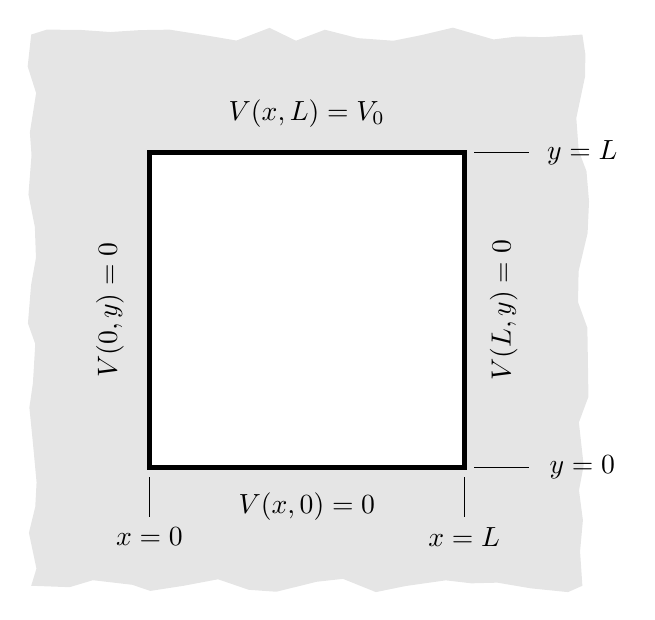
\begin{tikzpicture}
  \fill[gray!20, decoration={random steps,segment length=0.4cm}] (-1.5,-1.5) decorate{-- (+5.5,-1.5)} decorate{-- (+5.5,+5.5)} decorate{-- (-1.5,+5.5)} decorate{-- cycle};
  \draw[line width=0.6mm,fill=white] (0,0) -- (4,0) -- (4,4) -- (0,4) -- cycle;
  \node at (2,-0.5) {$V(x,0) = 0$};
  \node[rotate=90] at (-0.5,2) {$V(0,y) = 0$};
  \node[rotate=90] at ( 4.5,2) {$V(L,y) = 0$};
  \node at (2, 4.5) {$V(x,L) = V_0$}; 
%%%
  \draw (0,-0.125) -- (0,-0.625);
  \draw (4,-0.125) -- (4,-0.625);
  \node at (0,-0.875) {$x = 0$};
  \node at (4,-0.875) {$x = L$};   
%%%
  \draw (4.125,0) -- (4.825,0);
  \draw (4.125,4) -- (4.825,4);
  \node at (5.5,0) {$y = 0$};
  \node at (5.5,4) {$y = L$};  
\end{tikzpicture}
\caption{Illustration of a slice through an infinite square duct with prescribed electric potentials.}
\label{Fig:pde_illustration2DSquareCavity}
\end{center}
\end{figure}

%%%%%%%%%%%%%%%%%%%%%%%%%%%%%%%%%%%%%%%%%%%%%%%%%%%%%%%%%%%%%%%%%%%%%%%%%%%%%%%%%%%%%%%%%%%%%%%
\subsection{Example: Electric Field in an Infinite Square Duct}

The electric field in a steady-state problem is given by the gradient of a potential function:
\begin{align}
  \mathbf{E} = -\nabla V.
\end{align}
Taking the divergence of the electric field and applying Gauss' law gives
\begin{align}
  \nabla \cdot \mathbf{E} = -\nabla^2 V = \frac{\rho}{\epsilon_0} .
\end{align}

Now suppose we have a square duct with dimensions $0 \le x \le L$, $0 \le y \le L$ that is infinite and uniform in the $z$ direction. Within this duct, we will assume that there is no free electric charge. Finally, we will set one of the faces, $y = L$ to have an electric potential $V_0$ and the other faces set to zero. This problem is illustrated in Fig.~\ref{Fig:pde_illustration2DSquareCavity}.

The problem statement for the divergence of the electric field can be written as the Laplace equation for the electric potential function:
\begin{align}
  \dhotwo{V}{x} + \dhotwo{V}{y} = 0, \quad V(0,y) = V(L,y) = V(x,0) = 0, \quad V(x,L) = V_0 
\end{align}
on the domain $0 \le x \le L$, $0 \le y \le L$. We expect the derivative of the potential in $z$ to be zero because the prescribed potential function is uniform in the $z$ direction.

To begin, we assume the solution is separable in $x$ and $y$:
\begin{align}
  V(x,y) = X(x) Y(y) .
\end{align}
Inserting the proposed separable solution and dividing by $V(x,y) = X(x)Y(y)$ gives
\begin{align}
  \frac{1}{X} \dhotwo{X}{x} + \frac{1}{Y} \dhotwo{Y}{y} = 0.
\end{align}
Similar to the 1-D heat equation, we have a function of $x$ plus a function of $y$ is equal to zero. The difference being that each equation is now the same sign, which will be important for the form of the solution. The only way for this to be true is if both terms are equal to a constant:
\begin{subequations}
\begin{align}
  \frac{1}{X} \dhotwo{X}{x} &= K_1 \\*
  \frac{1}{Y} \dhotwo{Y}{y} &= K_2 .
\end{align}
\end{subequations}
From the partial differential equation we know that
\begin{align}
  K_1 = -K_2 ,
\end{align}
or that the constants are equal and opposite to one another. At this point, we must assess whether the constant $C_1$ is positive, negative, or zero by trying each of the cases. 

For the case where $K_1 = K_2 = 0$, we end up with
\begin{subequations}
\begin{align}
  \frac{1}{X} \dhotwo{X}{x} &= 0 \\*
  \frac{1}{Y} \dhotwo{Y}{y} &= 0 ,
\end{align}
\end{subequations}
which have the solutions
\begin{subequations}
\begin{align}
  X(x) &= A x + B \\*
  Y(y) &= C y + D .
\end{align}
\end{subequations}
Based on the boundary conditions in the $x$ coordinate, we have that $V(0,y) = V(L,y) = 0$. This gives the equations for $X(x)$ as
\begin{subequations}
\begin{align}
  X(0) &= B = 0 \\*
  X(L) &= A L + B  = 0.
\end{align}
\end{subequations}
From the first of these, we end up with $B = 0$. The second gives $A = 0$. This would imply that $X(x) = 0$ everywhere, meaning $V(x,y) = 0$ everywhere, which is not a solution that can satisfy the boundary condition $V(x,L) = V_0$. Because this would lead to an inconsistency, we reject the case where $K_1 = K_2 = 0$.

For the case where $K_1 > 0$, we set
\begin{align}
  K_1 &= k^2 , \nonumber \\*
  K_2 &= -k^2 . \nonumber
\end{align}
It follows that the solutions are
\begin{subequations}
\begin{align}
  X(x) &= A \sinh ( k x ) + B \cosh ( k x ) \\*
  Y(y) &= C \sin ( k y ) + D \cos ( k y ) .
\end{align}
\end{subequations}
From the boundary conditions $V(0,y) = V(L,y) = 0$, we have
\begin{subequations}
\begin{align}
  X(0) &= B = 0, \nonumber \\* 
  X(L) &= A \sinh ( k L ) = 0. \nonumber
\end{align}
\end{subequations}
The only way for
\begin{align}
  \sinh ( k L ) = 0 \nonumber
\end{align}
is for $k = 0$. (This contrasts with the trigonometric functions, which are periodic.) The other case is where $A = 0$. In both of these cases, this would again imply $X(x) = 0$ everywhere, or $V(x,y) = 0$ everywhere. This is, as before, inconsistent with the boundary condition $V(x,L) = V_0$ and therefore the case with $K_1 > 0$ must be rejected.

We therefore conclude that $K_1 < 0$. Before proceeding, it is worth noting that in our examples we ruled out the other two cases; however, as we say for the heat conduction problem, we did end up with parts of the solution that implicitly satisfied the $C_1 = 0$ case and led to the linear solution---we did this by separating out the transient from the steady state solutions, but the same result is true nonetheless. It is therefore necessary to consider all possible cases and include them in the solution.

Proceeding with $K_1 < 0$, we define
\begin{align}
  K_1 &= k^2 , \nonumber \\*
  K_2 &= -k^2 , \nonumber
\end{align}
which leads to the solutions
\begin{subequations}
\begin{align}
  X(x) &= A \sin ( k x ) + B \cos ( k x ) \\*
  Y(y) &= C \sinh ( k y ) + D \cosh ( k y ) .
\end{align}
\end{subequations}
Now as before, we apply the boundary conditions $V(0,y) = V(L,y) = 0$. For the first boundary condition at $x = 0$ we have
\begin{subequations}
\begin{align}
  X(0) = B = 0 .
\end{align}
For the second boundary condition at $x = L$ we have
\begin{align}
  X(L) = A \sin ( k L ) = 0 .
\end{align}
\end{subequations}
This can be true when $A = 0$, which yields the trivial solution or where $k L$ is an integer multiple of $\pi$. Therefore, as with the heat equation, we have
\begin{align}
  k_n = \frac{ n \pi }{ L }, \quad n = 1, 2, 3 \ldots
\end{align}
Therefore, for $C_1 < 0$, we do have meaningful solutions to the $X(x)$ equation. In fact, we have infinitely many solutions, so we include all of them as with the heat equation:
\begin{align}
  X(x) = \sum_{n=1}^\infty A_n \sin \left( \frac{n\pi x}{L} \right) .
\end{align}
The electric potential is therefore
\begin{align}
  V(x,y) = \sum_{n=1}^\infty A_n \sin \left( \frac{n\pi x}{L} \right) \left[ C \sinh \left( \frac{n\pi y}{L} \right) + D \cosh \left( \frac{n\pi y}{L} \right) \right] . 
\end{align}
Absorbing the constants we have
\begin{align}
  V(x,y) = \sum_{n=1}^\infty  \left[ C_n \sinh \left( \frac{n\pi y}{L} \right) + D_n \cosh \left( \frac{n\pi y}{L} \right) \right] \sin \left( \frac{n\pi x}{L} \right) .
\end{align}

Next, we must resolve the other two boundary conditions to solve for the remaining sets of constants. First, let us use $V(x,0) = 0$. This gives
\begin{align}
  V(x,0) = \sum_{n=1}^\infty  D_n \sin \left( \frac{n\pi x}{L} \right) = 0 .
\end{align}
The only way for this to be true is if all $D_n = 0$. Next, applying the $V(x,L) = V_0$ boundary condition gives
\begin{align}
  V(x,L) = \sum_{n=1}^\infty  C_n \sinh ( n \pi ) \sin \left( \frac{n\pi x}{L} \right) = V_0 .
\end{align}
Note that $C_n \sinh ( n \pi )$ is just a constant and that this has the expression of a Fourier series expansion. Therefore, this constant may be expressed as
\begin{align}
  C_n \sinh ( n \pi ) = \frac{2}{L} \int_0^L \sin \left( \frac{n\pi x}{L} \right) V_0 dx ,  \quad n = 1, 2, 3 \ldots 
\end{align}
Carrying out the integral gives
\begin{align}
  C_n \sinh ( n \pi ) = \frac{2 V_0}{n\pi} \left( 1 - \cos( n \pi) \right) ,  \quad n = 1, 2, 3 \ldots 
\end{align}
However, recall that for integer $n$
\begin{align}
  \cos ( n \pi ) = (-1)^n ,  \quad n = 1, 2, 3 \ldots  \nonumber
\end{align}
The term $1 - \cos(n \pi)$ is either 2 when $n$ is odd or 0 when $n$ is even. Therefore, we can write the constant as
\begin{align}
  C_n  = \left\{ \begin{array}{r l}
  \dfrac{4 V_0}{n\pi \sinh ( n \pi )}, & \quad n \text{ odd} \vspace{0.2cm} \\
  0, & \quad n \text{ even} \\ \end{array} \right. ,  \quad n = 1, 2, 3 \ldots 
\end{align}
Therefore, the solution for the electric potential is
\begin{align}
  V(x,y) = \sum_{\substack{n=1 \\ n \text{ odd}}}^\infty  \dfrac{4 V_0}{n\pi \sinh ( n \pi )} \sin \left( \frac{n\pi x}{L} \right) \sinh \left( \frac{n\pi y}{L} \right) .
\end{align}
Figure~\ref{Fig:pde_solution2DSquareCavity} shows an approximate solution with $N = 25$ terms in the expansion for $L = 4$ and $V_0 = 10$. As we can see, there are some spurious oscillations on the $(x,L)$ surface, however, overall it does line up with what we expect for the solution. Adding more terms would improve the smoothness of the plot.

The electric field is again $\mathbf{E} = -\nabla V$, therefore by taking the gradient we have
\begin{align}
  \mathbf{E}(x,y) = &-\sum_{\substack{n=1 \\ n \text{ odd}}}^\infty  \dfrac{4 V_0}{L \sinh ( n \pi )} 
  \left[ \cos \left( \frac{n\pi x}{L} \right) \sinh \left( \frac{n\pi y}{L} \right) \ihat + \sin \left( \frac{n\pi x}{L} \right) \cosh \left( \frac{n\pi y}{L} \right) \jhat \right] .
\end{align}

\begin{figure}[tb!]
\begin{center}
  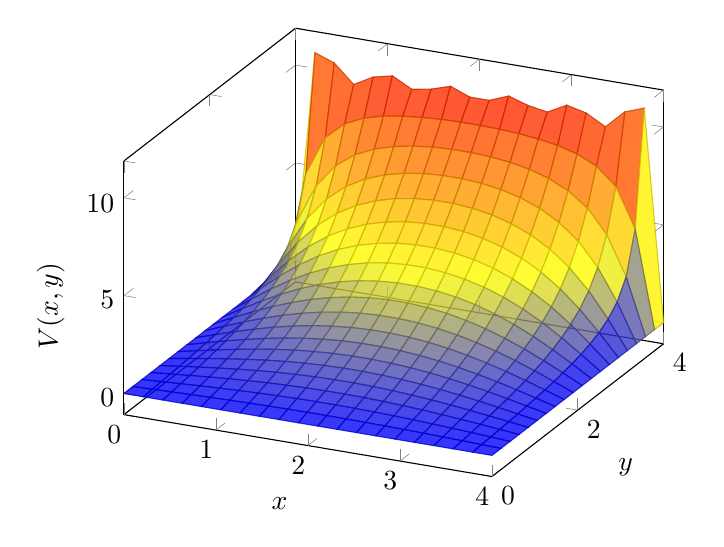
\begin{tikzpicture}[scale=1.0] 
  %\begin{axis}[xlabel=$x$,ylabel=$y$,view={0}{90}]
  \begin{axis}[xlabel=$x$,ylabel=$y$,zlabel={$V(x,y)$}]
  \addplot3[
    surf,
    opacity=0.8,
    samples=20, samples y=20,
    domain=0:4,domain y=0:4
  ]
 {40/pi*( sin(deg( 1*pi*x/4 )) * sinh( 1*pi*y/4 )/(1 * sinh( 1*pi ) )
        + sin(deg( 3*pi*x/4 )) * sinh( 3*pi*y/4 )/(3 * sinh( 3*pi ) ) 
        + sin(deg( 5*pi*x/4 )) * sinh( 5*pi*y/4 )/(5 * sinh( 5*pi ) )
        + sin(deg( 7*pi*x/4 )) * sinh( 7*pi*y/4 )/(7 * sinh( 7*pi ) )
        + sin(deg( 9*pi*x/4 )) * sinh( 9*pi*y/4 )/(9 * sinh( 9*pi ) )
        + sin(deg(11*pi*x/4 )) * sinh(11*pi*y/4 )/(11* sinh(11*pi ) )
        + sin(deg(13*pi*x/4 )) * sinh(13*pi*y/4 )/(13* sinh(13*pi ) )
        + sin(deg(15*pi*x/4 )) * sinh(15*pi*y/4 )/(15* sinh(15*pi ) ) 
        + sin(deg(17*pi*x/4 )) * sinh(17*pi*y/4 )/(17* sinh(17*pi ) )
        + sin(deg(19*pi*x/4 )) * sinh(19*pi*y/4 )/(19* sinh(19*pi ) )
        + sin(deg(21*pi*x/4 )) * sinh(21*pi*y/4 )/(21* sinh(21*pi ) )
        + sin(deg(23*pi*x/4 )) * sinh(23*pi*y/4 )/(23* sinh(23*pi ) )
        + sin(deg(25*pi*x/4 )) * sinh(25*pi*y/4 )/(25* sinh(25*pi ) ) ) };
  \end{axis}
  \end{tikzpicture}
\caption{Approximate solution for the electric potential of a 2-D slice within the square duct.}
\label{Fig:pde_solution2DSquareCavity}
\end{center}
\end{figure}


\begin{figure}[tb!]
\begin{center}
\begin{tikzpicture}
  \draw[line width=0.6mm,fill=gray!40] (0,0) -- (6,0) -- (6,4) -- (0,4) -- cycle;
  \node at (3,-0.5) {$T(x,-\tfrac{b}{2}) = T_0$};
  \node[rotate=90] at (-0.5,2) {$T(0,y) = 0$};
  \node[rotate=90] at ( 6.5,2) {$T(a,y) = 0$};
  \node at (3, 4.5) {$T(x,\tfrac{b}{2}) = T_0$}; 
%%%
  \draw (0,-0.125) -- (0,-0.625);
  \draw (6,-0.125) -- (6,-0.625);
  \node at (0,-0.875) {$x = 0$};
  \node at (6,-0.875) {$x = a$};   
%%%
  \draw (6.125,0) -- (6.825,0);
  \draw (6.125,4) -- (6.825,4);
  \node at (7.5,0) {$y = -\frac{b}{2}$};
  \node at (7.5,4) {$y =  \frac{b}{2}$};  
\end{tikzpicture}
\caption{Illustration of the first example for heat conduction on a 2-D rectangular plate.}
\label{Fig:pde_illustration2DRectangularPlate1}
\end{center}
\end{figure}

%%%%%%%%%%%%%%%%%%%%%%%%%%%%%%%%%%%%%%%%%%%%%%%%%%%%%%%%%%%%%%%%%%%%%%%%%%%%%%%%%%%%%%%%%%%%%%%
\subsection{Example: Heat Conduction on a Rectangular Plate}

Suppose we have a thin rectangular plate of thicknesses $a$ and $b$ in the $x$ and $y$ directions respectively. The plate is held at constant temperature zero on two of the left and right sides and $T_0$ at the top and bottom sides. This is depicted in Fig.~\ref{Fig:pde_illustration2DRectangularPlate1} and will be the first of two examples in this section.

We wish to obtain the temperature distribution $T(x,y)$ within the rectangular plate. To solve this problem, we define the origin in a specific way to simplify the boundary conditions using $0 \le x \le a$, and $-b/2 \le y \le b/2$ where
\begin{align}
  \dhotwo{T}{x} + \dhotwo{T}{y} = 0 , \quad T(0,y) = T(a,y) = 0, \quad T(x,-\tfrac{b}{2}) = T(x,\tfrac{b}{2}) = T_0 .
\end{align}
As with the electric potential problem, we assume a separable solution $T(x,y) = X(x) Y(y)$ and plug it into the differential equation to obtain
\begin{align}
  \frac{1}{X} \dhotwo{X}{x} + \frac{1}{Y} \dhotwo{Y}{y} = 0. \nonumber
\end{align}
The solutions have each term as equal and opposite constants $K_1$ and $K_2$. As before, we would attempt to find solutions satisfying the different boundary conditions that give the sign of the constants. We can reject $K_1 = 0$ and $K_1 > 0$ using the same arguments as with the electric potential problem, so they will not be repeated here. Using the $K_1 < 0$ case, everything is identical until we reach the point
\begin{align}
  T(x,y) = \sum_{n=1}^\infty  \left[ C_n \sinh \left( \frac{n\pi y}{a} \right) + D_n \cosh \left( \frac{n\pi y}{a} \right) \right] \sin \left( \frac{n\pi x}{a} \right) .
\end{align}
Now we must consider the boundary conditions $T(x,-b/2) = T(x,b/2) = T_0$. This gives a symmetric solution in $y$. Since the hyperbolic trigonometric functions are not periodic, only the hyperbolic cosine terms may satisfy this symmetry condition. We can therefore reject the odd functions in $y$ and set $C_n = 0$. This gives
\begin{align}
  T(x,y) = \sum_{n=1}^\infty  D_n \sin \left( \frac{n\pi x}{a} \right) \cosh \left( \frac{n\pi y}{a} \right)  .
\end{align}
Inserting either of the $T(x,-\tfrac{b}{2}) = T(x,\tfrac{b}{2}) = T_0$ gives
\begin{align}
  T(x,\pm \tfrac{b}{2}) = \sum_{n=1}^\infty  D_n \cosh \left( \frac{n\pi b}{2 a} \right) \sin \left( \frac{n\pi x}{a} \right) = T_0  .
\end{align}
As before, we recognize the terms on the left of the summation as constants that are coefficients in a Fourier series expansion. This gives the relationship
\begin{align}
  D_n \cosh \left( \frac{n\pi b}{2 a} \right) = \frac{2}{a} \int_0^a \sin \left( \frac{n\pi x}{a} \right) T_0 \hspace{0.2em} dx ,  \quad n = 1, 2, 3 \ldots 
\end{align}
which has the result
\begin{align}
  D_n  = \left\{ \begin{array}{r l}
  \dfrac{4 T_0}{n\pi \cosh ( \frac{n\pi b}{2 a} )}, & \quad n \text{ odd} \vspace{0.2cm} \\
  0, & \quad n \text{ even} \\ \end{array} \right. ,  \quad n = 1, 2, 3 \ldots 
\end{align}
This gives the solution for the temperature field as
\begin{align}
  T(x,y) = \sum_{\substack{n=1 \\ n \text{ odd}}}^\infty  \dfrac{4 T_0}{n\pi \cosh ( \frac{n\pi b}{2 a} ) } \sin \left( \frac{n\pi x}{a} \right) \cosh \left( \frac{n\pi y}{a} \right) .
\end{align}

This problem was largely identical to the previous problem except that the boundary condition was nonzero on the bottom surface. Because of the symmetry with the top surface, this motivated choosing the origin for $y$ to be at the center of the plate. This made the boundary conditions cause the hyperbolic sine term to vanish and yielded a solution that was largely identical to the other case except that the hyperbolic cosine term is used.

\begin{figure}[tb!]
\begin{center}
\begin{tikzpicture}
  \draw[line width=0.6mm,fill=gray!40] (0,0) -- (6,0) -- (6,4) -- (0,4) -- cycle;
  \node at (3,-0.5) {$T(x,-\tfrac{b}{2}) = T_0$};
  \node[rotate=90] at (-0.5,2) {$T(0,y) = 0$};
  \node[rotate=90] at ( 6.5,2) {$T(a,y) = 0$};
  \node at (3, 4.5) {$T(x,\tfrac{b}{2}) = 2 T_0$}; 
%%%
  \draw (0,-0.125) -- (0,-0.625);
  \draw (6,-0.125) -- (6,-0.625);
  \node at (0,-0.875) {$x = 0$};
  \node at (6,-0.875) {$x = a$};   
%%%
  \draw (6.125,0) -- (6.825,0);
  \draw (6.125,4) -- (6.825,4);
  \node at (7.5,0) {$y = -\frac{b}{2}$};
  \node at (7.5,4) {$y =  \frac{b}{2}$};  
\end{tikzpicture}
\caption{Illustration of the second example for heat conduction on a 2-D rectangular plate.}
\label{Fig:pde_illustration2DRectangularPlate2}
\end{center}
\end{figure}

Let us now consider another 2-D heat conduction problem with different boundary conditions
\begin{align}
  &\dhotwo{T}{x} + \dhotwo{T}{y} = 0 , \nonumber \\ &T(0,y) = T(a,y) = 0, \quad T(x,-\tfrac{b}{2}) = T_0, \quad T(x,\tfrac{b}{2}) = 2 T_0.
\end{align}
This problem is illustrated in Fig.~\ref{Fig:pde_illustration2DRectangularPlate2}.

To solve this problem, we apply the principle of superposition and write the temperature field as the sum of two temperature fields
\begin{align}
  T(x,y) = T_1(x,y) + T_2(x,y).
\end{align}
We define the temperature field $T_1(x,y)$ to satisfy the problem we just solved
\begin{align}
  \dhotwo{T_1}{x} + \dhotwo{T_1}{y} = 0 , \quad T_1(0,y) = T_1(a,y) = 0, \quad T_1(x,-\tfrac{b}{2}) = T_1(x,\tfrac{b}{2}) = T_0 .
\end{align}
It follows from what was done previously that the solution is
\begin{align}
  T_1(x,y) = \sum_{\substack{n=1 \\ n \text{ odd}}}^\infty  \dfrac{4 T_0}{n\pi \cosh ( \frac{n\pi b}{2 a} ) } \sin \left( \frac{n\pi x}{a} \right) \cosh \left( \frac{n\pi y}{a} \right) .
\end{align}
Now we build the problem for $T_2(x,y)$ by revisiting the differential equation
\begin{align}
  &\dhotwo{}{x} ( T_1 + T_2 ) + \dhotwo{}{y}( T_1 + T_2 )  = 0, \nonumber \\
  &\dhotwo{T_1}{x} + \dhotwo{T_1}{y} + \dhotwo{T_2}{x} + \dhotwo{T_2}{y} = 0. \nonumber
\end{align}
However, we know that the first two terms on the left-hand side are zero because of how the problem for $T_1(x,y)$ is defined. This gives the differential equation
\begin{align}
  \dhotwo{T_2}{x} + \dhotwo{T_2}{y} = 0 .
\end{align}
Now we must resolve the boundary conditions for $T_2(x,y)$. For the boundary condition at $(0,y)$ we have
\begin{subequations}
\begin{align}
  T(0,y) &= T_1(0,y) + T_2(0,y) = 0 + T_2(0,y) = 0 \nonumber \\
  T_2(0,y) &= 0.
\end{align}
It follows from the same line of reasoning that
\begin{align}
  T_2(a,y) &= 0 .
\end{align}
For the boundary condition $(x,-\tfrac{b}{2})$ we have
\begin{align}
  T(x,-\tfrac{b}{2}) &= T_1(x,-\tfrac{b}{2}) + T_2(x,-\tfrac{b}{2}) = T_0 + T_2(x,-\tfrac{b}{2}) = T_0 \nonumber \\
  T_2(x,\tfrac{b}{2}) &= 0.
\end{align}
And for the boundary condition $(x,\tfrac{b}{2})$ we have
\begin{align}
  T(x,\tfrac{b}{2}) &= T_1(x,\tfrac{b}{2}) + T_2(x,\tfrac{b}{2}) = T_0 + T_2(x,\tfrac{b}{2}) = 2 T_0 \nonumber \\
  T_2(x,\tfrac{b}{2}) &= T_0.
\end{align}
\end{subequations}
This gives a problem that is effectively identical to the 2-D electrostatic potential problem except for how the coordinate system is defined. To make this problem identical, we define a new coordinate system using the translation:
\begin{subequations}
\begin{align}
  u &= x, \\
  v &= y + \frac{b}{2} .
\end{align}
\end{subequations}
This leads to the problem
\begin{align}
  \dhotwo{T_2}{u} + \dhotwo{T_2}{v} = 0, \quad T_2(0,v) = T_2(a,v) = T_2(u,0) = 0, \quad T_2(u,b) = 1 . 
\end{align}
From our electrostatics problem, we obtain the equivalent solution:
\begin{align}
  T_2(u,v) = \sum_{\substack{n=1 \\ n \text{ odd}}}^\infty  \dfrac{4 T_0}{n\pi \sinh ( \frac{n \pi b}{a} )} \sin \left( \frac{n\pi u}{a} \right) \sinh \left( \frac{n\pi v}{a} \right) .
\end{align}
Substituting in values of $x$ and $y$ gives
\begin{align}
  T_2(x,y) = \sum_{\substack{n=1 \\ n \text{ odd}}}^\infty  \dfrac{4 T_0}{n\pi \sinh ( \frac{n \pi b}{a} )} \sin \left( \frac{n\pi x}{a} \right) \sinh \left( \frac{n\pi ( y + \frac{b}{2} )}{a} \right) .
\end{align}

Applying superposition, we can arrive at our combined solution for the temperature field
\begin{align}
  T(x,y) =  \sum_{\substack{n=1 \\ n \text{ odd}}}^\infty  \dfrac{4 T_0}{n\pi} \sin \left( \frac{n\pi x}{a} \right)
  \left[ \frac{  \cosh \left( n\pi y / a \right) }{ \cosh ( n\pi b/(2 a) ) } + \frac{ \sinh \left( n\pi ( y + \frac{b}{2} )/a \right) }{ \sinh ( n \pi b/a ) } \right] .
\end{align}
An approximation solution using $N = 15$ is plotted in Fig.~\ref{Fig:pde_solution2DrectangularPlate} using the values of $a = 3$, $b = 2$, and $T_0 = 100$. As with the 2-D electrostatics problem, the solution exhibits spurious oscillations that would diminish as $N$ becomes very large. The solution does, however, follow the general trends of satisfying the boundary conditions with zero on the sides, and $T = 100$ and $T = 200$ on the other two ends.

\begin{figure}[tb!]
\begin{center}
  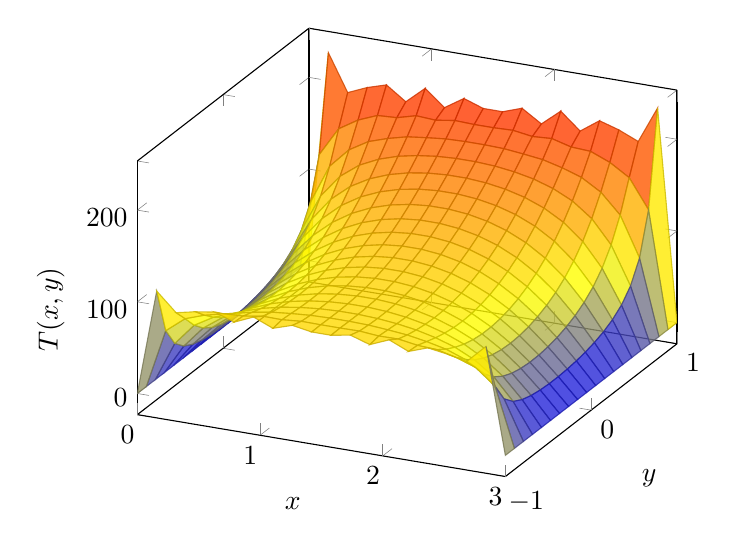
\begin{tikzpicture}[scale=1.0] 
  %\begin{axis}[xlabel=$x$,ylabel=$y$,view={0}{90}]
  \begin{axis}[xlabel=$x$,ylabel=$y$,zlabel={$T(x,y)$}]
  \addplot3[
    surf,
    opacity=0.8,
    samples=20, samples y=20,
    domain=0:3,domain y=-1:1
  ]
 {400/pi*( sin(deg( 1*pi*x/3 ))/ 1 * ( cosh( 1*pi*y/3)/cosh( 1*pi*2/6 ) + sinh( 1*pi*(y + 1)/3)/sinh( 1*pi*2/3) ) 
         + sin(deg( 3*pi*x/3 ))/ 3 * ( cosh( 3*pi*y/3)/cosh( 3*pi*2/6 ) + sinh( 3*pi*(y + 1)/3)/sinh( 3*pi*2/3) )  
         + sin(deg( 5*pi*x/3 ))/ 5 * ( cosh( 5*pi*y/3)/cosh( 5*pi*2/6 ) + sinh( 5*pi*(y + 1)/3)/sinh( 5*pi*2/3) )  
         + sin(deg( 7*pi*x/3 ))/ 7 * ( cosh( 7*pi*y/3)/cosh( 7*pi*2/6 ) + sinh( 7*pi*(y + 1)/3)/sinh( 7*pi*2/3) )  
         + sin(deg( 9*pi*x/3 ))/ 9 * ( cosh( 9*pi*y/3)/cosh( 9*pi*2/6 ) + sinh( 9*pi*(y + 1)/3)/sinh( 9*pi*2/3) )  
         + sin(deg(11*pi*x/3 ))/11 * ( cosh(11*pi*y/3)/cosh(11*pi*2/6 ) + sinh(11*pi*(y + 1)/3)/sinh(11*pi*2/3) )  
         + sin(deg(13*pi*x/3 ))/13 * ( cosh(13*pi*y/3)/cosh(13*pi*2/6 ) + sinh(13*pi*(y + 1)/3)/sinh(13*pi*2/3) )  
         + sin(deg(15*pi*x/3 ))/15 * ( cosh(15*pi*y/3)/cosh(15*pi*2/6 ) + sinh(15*pi*(y + 1)/3)/sinh(15*pi*2/3) )  ) };
  \end{axis}
  \end{tikzpicture}
\caption{Approximate solution for the temperature field on a rectangular plate for the second example problem.}
\label{Fig:pde_solution2DrectangularPlate}
\end{center}
\end{figure}


%%%%%%%%%%%%%%%%%%%%%%%%%%%%%%%%%%%%%%%%%%%%%%%%%%%%%%%%%%%%%%%%%%%%%%%%%%%%%%%%%%%%%%%%%%%%%%%
\subsection{Example: Electric Field in a Semi-infinite Rectangular Duct}

Now consider the case where we have a square 3-D duct with $0 \le x \le a$, $0 \le y \le b$, defined over the right half-space in the $z$ direction such that $0 \le z < \infty$. We set the electric potential to zero on all faces except for the $z = 0$ face, which we set to some constant $V_0$. The equation for the electrostatic potential is
\begin{align}
  &\dhotwo{V}{x} + \dhotwo{V}{y} + \dhotwo{V}{z} = 0, \nonumber \\
  &V(0,y,z) = V(a,y,z) = V(x,0,z) = V(x,b,z) = 0, \nonumber \\
  &V(x,y,0) = V_0, \quad V(x,y,z) \rightarrow 0, z \rightarrow \infty .
\end{align}
Since the electric potential function should be similar to the adjacent faces, we have the potential going to zero as we get far away from the $z = 0$ face.

To solve this problem, we apply separation of variables
\begin{align}
  V(x,y,z) = X(x) Y(y) Z(z) .
\end{align}
Inserting this into the differential equation and dividing by $V = XYZ$ we get
\begin{align}
  \frac{1}{X} \dhotwo{X}{x} + \frac{1}{Y} \dhotwo{Y}{y} + \frac{1}{Z} \dhotwo{Z}{z} = 0.
\end{align}
Analogous to the 2-D case, we have a function of $x$ plus a function of $y$ plus a function of $z$ is equal to zero. This can only be true if each of the functions are equal to constants:
\begin{subequations}
\begin{align}
  \frac{1}{X} \dhotwo{X}{x} &= K_1, \\
  \frac{1}{Y} \dhotwo{Y}{y} &= K_2, \\
  \frac{1}{Z} \dhotwo{Z}{z} &= K_3.  
\end{align}
\end{subequations}
We now must determine the signs of the constants. This laborious step is omitted here, but from prior experience with the 2-D cases, we can surmise that $K_1 < 0$ and $K_2 < 0$. Given that
\begin{align}
  K_1 + K_2 + K_3 = 0, \nonumber
\end{align}
we know that $K_3 > 0$. We define
\begin{subequations}
\begin{align}
  \frac{1}{X} \dhotwo{X}{x} &= -k^2, \\
  \frac{1}{Y} \dhotwo{Y}{y} &= -\ell^2 ; 
\end{align}
\end{subequations}
this gives the following solutions
\begin{subequations}
\begin{align}
  X(x) = A \sin( k x ) + B \cos ( k x ), \\
  Y(y) = C \sin( \ell y ) + D \cos ( \ell y ) .
\end{align}
\end{subequations}
It follows for the $z$ equation that
\begin{align}
  \frac{1}{Z} \dhotwo{Z}{z} &= k^2 + \ell^2 ,
\end{align}
which gives the solution
\begin{align}
  Z(z) = F e^{\sqrt{ k^2 + \ell^2 } z} + G e^{-\sqrt{ k^2 + \ell^2 } z} . 
\end{align}
Here we use exponentials rather than hyperbolic trigonometric functions because of the boundary condition that as $z \rightarrow \infty$, the potential goes to zero. This implies that $F = 0$, giving the result
\begin{subequations}
\begin{align}
  Z(z) = G e^{-\sqrt{ k^2 + \ell^2 } z} .
\end{align}
By applying the boundary conditions at $x = 0$ and $y = 0$, we can show that the coefficients $B = 0$ and $D = 0$ respectively. Giving us
\begin{align}
  X(x) = A \sin( k x ) , \\
  Y(y) = C \sin( \ell y ) .
\end{align}
\end{subequations}
Using the boundary conditions at $x = a$ and $y = b$, gives the familiar result that $k$ and $\ell$ must be integer multiples of $\pi$. That is
\begin{subequations}
\begin{align}
  k_n &= \frac{n\pi}{a}, \quad n = 1, 2, 3 \ldots \\
  \ell_n &= \frac{m\pi}{b}, \quad m = 1, 2, 3 \ldots 
\end{align}
\end{subequations}
Therefore, we have infinitely many values of $k$ and $\ell$ that yield the solution and we can take a linear combination of those solutions
\begin{subequations}
\begin{align}
  X(x) = \sum_{n=1}^\infty A_n \sin \left( \frac{ n \pi x }{ a } \right) , \\
  Y(y) = \sum_{m=1}^\infty C_m \sin \left( \frac{ m \pi y }{ b } \right) .
\end{align}
\end{subequations}
The solution for the electric potential is therefore
\begin{align}
  V(x,y,z) = \sum_{n=1}^\infty A_n \sin \left( \frac{ n \pi x }{ a } \right) \sum_{m=1}^\infty C_m \sin \left( \frac{ m \pi y }{ b } \right) 
  G \exp \left[ -\sqrt{ \left( \frac{ n \pi }{ a } \right)^2 + \left( \frac{ m \pi }{ b } \right)^2 }  z \right] . \nonumber
\end{align}
Combining the constants and rearranging gives
\begin{align}
  V(x,y,z) = \sum_{n=1}^\infty \sum_{m=1}^\infty A_{n,m} \sin \left( \frac{ n \pi x }{ a } \right)  \sin \left( \frac{ m \pi y }{ b } \right) 
  \exp \left[ -\sqrt{ \left( \frac{ n \pi }{ a } \right)^2 + \left( \frac{ m \pi }{ b } \right)^2 }  z \right] . 
\end{align}
Here $A_{n,m}$ is a combined constant that depends upon both indices. We have one remaining boundary condition to determine this constant, $V(x,y,0) = V_0$. Plugging this in gives
\begin{align}
  V(x,y,0) = \sum_{n=1}^\infty \sum_{m=1}^\infty A_{n,m} \sin \left( \frac{ n \pi x }{ a } \right)  \sin \left( \frac{ m \pi y }{ b } \right) = V_0 . 
\end{align}
We can obtain this constant by multiplying by products of sine functions in indices $\nu$ and $\mu$ and then integrating $x$ from 0 to $a$ and $y$ form 0 to $b$:
\begin{align}
  &\sum_{n=1}^\infty \sum_{m=1}^\infty A_{n,m} \int_0^a \sin \left( \frac{ \nu \pi x }{ a } \right) \sin \left( \frac{ n \pi x }{ a } \right) dx \int_0^b  \sin \left( \frac{ \mu \pi y  }{ b } \right) \sin \left( \frac{ m \pi y }{ b } \right) dy \nonumber \\
  &= \int_0^a \int_0^b V_0 \sin \left( \frac{ \nu \pi x }{ a } \right)  \sin \left( \frac{ \mu \pi y  }{ b } \right) dy dx .
\end{align}
Using the orthogonality property, we know that all but the terms where $n = \nu$ and $m = \mu$ survive in the inner product. This gives
\begin{align}
  A_{n,m} \left( \frac{a}{2} \right) \left( \frac{b}{2} \right) = \int_0^a \int_0^b V_0 \sin \left( \frac{ n \pi x }{ a } \right)  \sin \left( \frac{ m \pi y  }{ b } \right) dy dx .
\end{align}
Performing the integral and solving for the constant gives
\begin{align}
  A_{n,m} = \left\{ \begin{array}{r l}
  \dfrac{16 V_0}{\pi^2 n m }, & \quad \text{ both $n$ and $m$ odd} \vspace{0.2cm} \\
  0, & \quad \text{ either $n$ or $m$ even} \\ \end{array} \right. .
\end{align}
The electric potential function is therefore
\begin{align}
  V(x,y,z) = \sum_{\substack{n=1 \\ n \text{ odd}}}^\infty \sum_{\substack{m=1 \\ m \text{ odd}}}^\infty  &\frac{16 V_0}{\pi^2 n m } \sin \left( \frac{ n \pi x }{ a } \right)  \sin \left( \frac{ m \pi y }{ b } \right)  \exp \left[ -\sqrt{ \left( \frac{ n \pi }{ a } \right)^2 + \left( \frac{ m \pi }{ b } \right)^2 }  z \right] . 
\end{align}
The electric field may be obtained by $\mathbf{E} = -\nabla V$.


%%%%%%%%%%%%%%%%%%%%%%%%%%%%%%%%%%%%%%%%%%%%%%%%%%%%%%%%%%%%%%%%%%%%%%%%%%%%%%%%%%%%%%%%%%%%%%%
\subsection{Spherical Coordinates and Legendre Polynomials}

Previously we had considered solving the Laplace equation in Cartesian coordinates. We now turn our attention to spherical coordinates. (Cylindrical coordinates require special functions called Bessel functions, and are not covered.) The Laplace equation in spherical coordinates is
\begin{align}
  \frac{1}{r^2} \dho{}{r} \left( r^2 \dho{u}{r} \right) 
               + \frac{1}{r^2 \sin \theta } \dho{}{\theta} \left( \sin \theta \dho{u}{\theta} \right) 
               + \frac{1}{r^2 \sin^2 \theta } \dhotwo{u}{\phi} = 0
\end{align}
with boundary conditions prescribed as appropriate.

This equation is quite complicated. We can simplify it significantly if we restrict ourselves to problems that are azimuthally symmetric. This allows us to remove the derivative in $\phi$ to yield the Laplace equation for spherical coordinates with azimuthally symmetry:
\begin{align}
  \frac{1}{r^2} \dho{}{r} \left( r^2 \dho{u}{r} \right) 
               + \frac{1}{r^2 \sin \theta } \dho{}{\theta} \left( \sin \theta \dho{u}{\theta} \right) = 0 .
\end{align}
As with the Cartesian case, we assume that the solution is separable and write
\begin{align}
  u(r,\theta) = R(r) \Theta(\theta) .
\end{align}
Inserting this into the differential equation and dividing by $u = R \Theta$ gives the equation
\begin{align}
  \frac{1}{R} \dho{}{r} \left( r^2 \dho{R}{r} \right) 
               + \frac{1}{\Theta \sin \theta } \dho{}{\theta} \left( \sin \theta \dho{\Theta}{\theta} \right) = 0 .
\end{align}
Here the $1/r^2$ term has been multiplied away.

Since we have a function of $r$ plus a function of $\theta$ equals zero, we know that each of the terms must equal to a constant $K$ and that those constants are equal and opposite. As with Cartesian coordinates we must deduce the sign of $K$. The sign of $K$ that produces sensible results is to assign the positive term to the radial $R$ equation and the negative term to the polar $\Theta$ equation:
\begin{subequations}
\begin{align}
  &\frac{1}{R} \dho{}{r} \left( r^2 \dho{R}{r} \right) = K, \\\
  &\frac{1}{\Theta \sin \theta } \dho{}{\theta} \left( \sin \theta \dho{\Theta}{\theta} \right) = -K .
\end{align}
\end{subequations}
Therefore, when we expand out these equations, we have
\begin{subequations}
\begin{align}
  &r^2 \dhotwo{R}{r} + 2 r \dho{R}{r} - K R(r) = 0, \\
  &\dhotwo{\Theta}{\theta} + \frac{ \cos \theta }{ \sin \theta } \dho{\Theta}{\theta} + K \Theta(\theta) = 0.
\end{align}
\end{subequations}


These equations are unwieldy, and their solutions are certainly not obvious. First, we will focus our attention on the $\Theta$ equation. It turns out (again, not obvious) that the equation only has a solution when 
\begin{align}
  K = \ell ( \ell + 1 ), \quad \ell = 0, 1, 2 \ldots
\end{align}
and the solutions correspond to a special set of polynomials we denote by $P_\ell(\cos \theta)$, where $\ell$ represents the highest order term in the polynomial. These polynomials are called the \emph{Legendre polynomials}, and like the trigonometric functions form a complete an orthogonal basis. Let us now briefly turn our attention away from the spherical Laplace equation and discuss the Legendre polynomials.

Suppose we wish to construct a series of orthogonal polynomial functions defined on the domain $-1 \le \mu \le 1$. (If the domain is not $-1$ to $1$, we can always transform the coordinates to make it as such.) The simplest polynomial is a constant equal to one, so we start by defining
\begin{align}
  P_0(\mu) = 1. \nonumber
\end{align}
Now we wish to find a polynomial of degree $\ell = 1$, call it $P_1(\mu)$, such that
\begin{align}
  \int_{-1}^1 P_1(\mu) P_0(\mu) d\mu &= 0, \nonumber \\
  \int_{-1}^1 P_1(\mu) P_1(\mu) d\mu &= c_1 \ne 0 . \nonumber
\end{align}
To satisfy the first constraint, we require the polynomial be odd or be symmetric about the origin. A polynomial that meets this criterion is
\begin{align}
  P_1(\mu) = \mu . \nonumber
\end{align}
We could apply a multiplicative constant and still meet this constraint, but it turns out that as we go further, having a multiplicative constant of one is the right choice. We then continue and attempt to find a quadratic polynomial $P_2(\mu)$ that now satisfies the constraints
\begin{align}
  \int_{-1}^1 P_2(\mu) P_0(\mu) d\mu &= 0, \nonumber \\
  \int_{-1}^1 P_2(\mu) P_1(\mu) d\mu &= 0, \nonumber \\
  \int_{-1}^1 P_2(\mu) P_2(\mu) d\mu &= c_2 \ne 0 . \nonumber
\end{align}
A polynomial that does this is
\begin{align}
  P_2(\mu) = \frac{1}{2} \left( 3 \mu^2 - 1 \right) . \nonumber
\end{align}
We continue this process to construct a series of polynomials satisfying the orthogonality property
\begin{align}
  \int_{-1}^1 P_\ell(\mu) P_m(\mu) d\mu = \frac{ 2 }{ 2 \ell + 1 } \delta_{\ell m} ,
\end{align}
where here we have explicitly wrote out the constant that we will enforce.

Continuing this process, we can deduce the following definition of the Legendre polynomials:
\begin{subequations}
\begin{align}
  P_0(\mu) &= 1, \\
  P_1(\mu) &= \mu, \\
  P_{\ell+1}(\mu) &= \frac{ ( 2\ell + 1 ) \mu P_\ell(\mu) - \ell P_{\ell - 1}( \mu ) }{ \ell + 1 } , \quad \ell \ge 1.
\end{align}
\end{subequations}
The last of these is a recursion relationship that allows us to generate any order polynomial $\ell \ge 2$.

As we mentioned previously, the Legendre polynomials form a complete an orthogonal basis. Therefore, similar to Fourier expansions, we can take Legendre polynomial expansions of functions defined on the domain $-1 \le \mu \le 1$:
\begin{align}
  f(\mu) = \sum_{\ell=0}^\infty \left( \frac{ 2\ell + 1 }{ 2 } \right) f_\ell P_\ell(\mu) .
\end{align}
The expansion coefficient $f_\ell$ (sometimes called the Legendre moment) can be obtained from
\begin{align}
  f_\ell = \int_{-1}^1 f(\mu) P_\ell(\mu) d\mu .
\end{align}

As an aside, the Legendre polynomials have many applications outside solving the Laplace equation. For example, they are frequently used in performing fast integration method called the Gauss-Legendre quadrature scheme. In fact, we can very rapidly integrate polynomials exactly on a computer by evaluating the function at roots of a certain order of the Legendre polynomials multiplying by special weighting factors and adding up the results. The Gauss-Legendre quadrature is one of most efficient tools for numerical integration available. Another application of Legendre polynomials and their expansions is in radiation interactions with matter. The change in direction that a photon or neutron experiences in a scattering event is random and often well described by an expansion in Legendre polynomials.

Returning to the Laplace equation, applying the Legendre polynomials we let $\mu = \cos \theta$ and we have that solution for $\Theta(\theta)$ is
\begin{align}
  \Theta(\theta) = C_\ell P_\ell(\cos \theta), \quad \ell = 0, 1, 2 \ldots
\end{align}
where $C_\ell$ is some arbitrary constant. Before moving onto the radial equation. It is worth noting that, being a second-order ordinary differential equation, we expect there to be two sets of solutions to $\Theta(\theta)$. Indeed there is, and this is called the \emph{Legendre function of the second kind} given by $Q_\ell(\cos \theta)$. The first couple Legendre functions of the second kind in terms of $\mu$ is
\begin{subequations}
\begin{align}
  Q_0(\mu) &=   \frac{1}{2} \ln \left( \frac{ 1 + \mu }{ 1 - \mu } \right) , \\
  Q_1(\mu) &= \frac{\mu}{2} \ln \left( \frac{ 1 + \mu }{ 1 - \mu } \right) - 1 .
\end{align}
\end{subequations}
The higher-order Legendre functions of the second kind satisfy the same recursion relationship as the Legendre polynomials. Note that the $Q_\ell(\cos \theta)$ functions blow up as $\theta$ approaches $0$ to $2\pi$. Therefore, the Legendre function can often be rejected because we normally require that the solution be finite, unless we have a case where the polar axis is not included in the problem domain for some reason. For completeness the solution to the polar equation is
\begin{align}
  \Theta(\theta) = C_\ell P_\ell(\cos \theta) + D_\ell Q_\ell(\cos \theta), \quad \ell = 0, 1, 2 \ldots
\end{align}
even through the second term is seldom required.

Since $\mu = \cos \theta$ then it will be convenient to rewrite the equations for the Legendre polynomials in terms of $\theta$. The orthogonality property becomes
\begin{align}
  \int_0^\pi P_\ell ( \cos \theta ) P_m ( \cos \theta ) \sin \theta d\theta = \frac{2}{2\ell + 1} \delta_{\ell m} ;
\end{align}
the Legendre polynomial expansion is
\begin{align}
  f(\cos \theta) = \sum_{\ell = 0}^\infty \left( \frac{ 2 \ell + 1 }{2 } \right) f_\ell P_\ell(\cos \theta) ;
\end{align}
and the expansion coefficient is
\begin{align}
  f_\ell = \int_0^\pi f(\cos \theta) P_\ell(\cos \theta) \sin \theta d\theta .
\end{align}

Moving on to the radial equation, we have with the choice of constant that satisfies $\Theta(\theta)$:
\begin{align}
  r^2 \dhotwo{R}{r} + 2 r \dho{R}{r} - \ell ( \ell + 1 ) R(r) = 0 .
\end{align}
The solution to this equation is also not obvious, but we can verify that
\begin{align}
  R(r) = A_\ell r^\ell + B_\ell \frac{1}{r^{\ell+1}}, \quad \ell = 0, 1, 2 \ldots
\end{align}
does indeed satisfy the differential equation for $R(r)$.

Multiplying our solutions for $R(r)$ and $\Theta(\theta)$ together and combining constants, we have the solution for the Laplace equation in spherical coordinates with azimuthal symmetry as
\begin{align}
  u(r,\theta) = \sum_{\ell = 0}^\infty \left( A_\ell r^\ell + B_\ell \frac{1}{r^{\ell+1}} \right) P_\ell( \cos \theta ) .
\end{align}
Since there are infinitely many integer values of $\ell$ that satisfy the equation, we take a linear combination of all possible solutions. We will then need to apply the boundary conditions to solve for the coefficients. Let us illustrate this with a few examples.

%%%%%%%%%%%%%%%%%%%%%%%%%%%%%%%%%%%%%%%%%%%%%%%%%%%%%%%%%%%%%%%%%%%%%%%%%%%%%%%%%%%%%%%%%%%%%%%
\subsection{Example: Heat Conduction in a Sphere}

Suppose we have a sphere of radius $a$ where the temperature is specified on the exterior of the sphere at $r = a$ as a function of $\theta$. The Laplace equation can be used as before to solve the heat conduction, but this time in spherical coordinates:
\begin{align}
  \frac{1}{r^2} \dho{}{r} \left( r^2 \dho{T}{r} \right) 
               + \frac{1}{r^2 \sin \theta } \dho{}{\theta} \left( \sin \theta \dho{T}{\theta} \right) = 0 , \quad T(a,\theta) = f(\theta), \quad 0 \le r \le a .
\end{align}
We will not repeat the separation of variables, as it is the same as what was just discussed, and simply write out the form of the solution:
\begin{align}
  T(r,\theta) = \sum_{\ell = 0}^\infty \left( A_\ell r^\ell + B_\ell \frac{1}{r^{\ell+1}} \right) P_\ell( \cos \theta ) . \nonumber
\end{align}
We must now apply the boundary conditions to resolve the coefficients.

First, we know the temperature must be finite everywhere and the domain includes $r = 0$. The terms in
\begin{align}
  B_\ell \frac{1}{r^{\ell + 1}}, \quad \ell = 0, 1, 2 \ldots \nonumber
\end{align}
always diverge as $r \rightarrow 0$. For this reason, we must exclude them and we do this by setting $B_\ell = 0$ for all values of $\ell$.

Applying the boundary condition at $r = a$ gives
\begin{align}
  f(\theta) = \sum_{\ell = 0}^\infty A_\ell a^\ell P_\ell( \cos \theta ) . 
\end{align}
This is a a Legendre polynomial expansion if we let
\begin{align}
  A_\ell a^\ell = \left( \frac{ 2 \ell + 1 }{2 } \right) f_\ell 
\end{align}
Applying the relationship for the Legendre coefficient and solving for the integration constant gives the result:
\begin{align}
  A_\ell  = \left( \frac{ 2 \ell + 1 }{2 a^\ell } \right) \int_0^\pi f(\theta) P_\ell(\cos \theta) \sin \theta d\theta .
\end{align}

In general, we would need to carry out the integrals (often numerically) to find the coefficients. Fortunately, it is often the case where $f(\theta)$ has a form where the $\theta$ having only the dependence of $\cos^n \theta$ where $n$ are non-negative integers. In this case, we can avoid doing the integrals and ``pick out'' the coefficients directly by starting with the highest order term and working down to the constant.

To illustrate, consider the boundary condition:
\begin{align}
  f(\theta) = 1 - \cos \theta + 3 \cos^2 \theta .
\end{align}
Here the highest-order term in $\cos \theta$ is 2. Therefore we try to write the equation in terms of the second-order Legendre polynomial
\begin{align}
   P_2(\cos \theta) = \frac{1}{2} \left( 3 \cos^2 \theta - 1 \right) . \nonumber
\end{align}
To do this, we multiply and divide the $\cos^2 \theta$ term by $2$:
\begin{align}
  f(\theta) = 1 - \cos \theta + 2 \cdot \frac{1}{2} \left( 3 \cos^2 \theta \right) . \nonumber
\end{align}
Then we add an subtract $1$ inside the parentheses to get 
\begin{align}
  f(\theta) = 1 - \cos \theta + 2 \cdot \frac{1}{2} \left( 3 \cos^2 \theta - 1  \right) + 1. \nonumber
\end{align}
Recognizing $P_2(\cos \theta)$ and regrouping terms gives
\begin{align}
  f(\theta) = 2 - \cos \theta + 2 P_2( \cos \theta ). \nonumber
\end{align}
Noting that $P_0(\cos \theta) = 1$ and $P_1(\cos \theta) = \cos \theta$ we can write this as
\begin{align}
  f(\theta) = 2 P_0( \cos \theta) - P_1( \cos \theta)  + 2 P_2( \cos \theta ) =  \sum_{\ell = 0}^\infty A_\ell a^\ell P_\ell( \cos \theta ) .
\end{align}
Therefore, the coefficients are
\begin{subequations}
\begin{align}
  A_0 &= 2, \\
  A_1 &= -\frac{1}{a}, \\
  A_2 &= \frac{2}{a^2}, \\
  A_\ell &= 0, \quad \ell > 2
\end{align}
\end{subequations}
The temperature within the sphere is therefore
\begin{align}
  T(r,\theta) = 2 - \frac{r}{a} \cos \theta + \frac{r^2}{a^2} \left( 3 \cos^2 \theta - 1 \right) .
\end{align}


%%%%%%%%%%%%%%%%%%%%%%%%%%%%%%%%%%%%%%%%%%%%%%%%%%%%%%%%%%%%%%%%%%%%%%%%%%%%%%%%%%%%%%%%%%%%%%%
\subsection{Example: Fluid Velocity Around a Spinning Ball}

Suppose we have a solid ball or radius $a$ immersed in large vat containing a viscous fluid such that it is centered at the origin of a spherical coordinate system. Suppose the ball spins about the $z$ axis such that the velocity of the ball at the surface has an azimuthal component
\begin{align}
  u_\phi(a,\theta) = a \omega \sin \theta .
\end{align}
Here $\omega$ is the angular velocity. The ball rotates with an azimuthal velocity that is faster at the equator than near the poles. We can assume the vat is large and fluid is stagnant so that faraway from the ball, the azimuthal velocity is zero, $u_\phi(\infty,\theta) = 0$.

If we assume that the fluid is sufficiently viscous and $\omega$ is sufficiently small so that we can neglect turbulence, then the azimuthal velocity is described by the Laplace equation in spherical coordinates. Because the rotation is azimuthally symmetric, the azimuthal component of the fluid velocity is azimuthally constant and only depends on the radial position and the polar angle with respect to the axis of rotation. The differential equation is therefore
\begin{align}
  &\frac{1}{r^2} \dho{}{r} \left( r^2 \dho{u_\phi}{r} \right) 
               + \frac{1}{r^2 \sin \theta } \dho{}{\theta} \left( \sin \theta \dho{u_\phi}{\theta} \right) = 0 , \nonumber \\
               &u_\phi(a,\theta) = a \omega \sin \theta, \quad u_\phi(\infty,\theta) = 0, \quad \quad r \ge a .
\end{align}

As we have seen, the solution is 
\begin{align}
  u_\phi(r,\theta) = \sum_{\ell = 0}^\infty \left( A_\ell r^\ell + B_\ell \frac{1}{r^{\ell+1}} \right) P_\ell( \cos \theta ) .
\end{align}
This time, because the domain does not include the origin, we cannot eliminate the $B_\ell$ terms. On the other hand, what we can do is eliminate the $A_\ell$ terms, as this is the only way for the solution to go to zero for large $r$. Applying the boundary condition at the surface of the sphere gives
\begin{align}
  u_\phi(a,\theta) =  \sum_{\ell = 0}^\infty B_\ell \frac{1}{a^{\ell+1}} P_\ell( \cos \theta ) = a \omega \sin \theta .
\end{align}
We recognize that this is a Legendre polynomial expansion if we equate
\begin{align}
  B_\ell \frac{1}{a^{\ell + 1}} = \left( \frac{ 2 \ell + 1 }{2 } \right) f_\ell .
\end{align}
Solving for the integration constant and writing the equation in terms of the integral for the expansion coefficient gives
\begin{align}
  B_\ell  = a^{\ell+2} \omega \left( \frac{ 2 \ell + 1 }{2 } \right) \int_0^\pi \sin \theta P_\ell(\cos \theta) \sin \theta d\theta , \nonumber
\end{align}

At this point, let us check if we can equate terms as we did in the previous example. Unfortunately, by
\begin{align}
  \cos^2 \theta + \sin^2 \theta = 1 \nonumber
\end{align}
we would get 
\begin{align}
  B_\ell  = a^{\ell+2} \omega \left( \frac{ 2 \ell + 1 }{2 } \right) \int_0^\pi \sqrt{ 1 - \cos \theta } P_\ell(\cos \theta) \sin \theta d\theta , \nonumber
\end{align}
which does not depend upon only nonnegative integer powers of $\cos \theta$. Therefore, we will be unable to write the expansion exactly for at a finite number of terms. Rather, we will need to estimate the terms directly and truncate at a certain point. On the bright side, because $\sin^2 \theta$ is an even function, we know that only the even values of the expansion will be nonzero. Evaluating the integral
\begin{align}
  B_\ell  = a^{\ell+2} \omega \left( \frac{ 2 \ell + 1 }{2 } \right) \int_0^\pi \sin^2 \theta P_\ell(\cos \theta)  d\theta
\end{align}
for the first few even values of $\ell$ gives
\begin{subequations}
\begin{align}
  B_0 &= \frac{ \pi a^2 \omega }{ 4 } , \\
  B_2 &= -\frac{ 5 \pi a^4 \omega }{ 32 }, \\
  B_4 &= -\frac{ 9 \pi a^6 \omega }{ 256 }, \\
  B_6 &= -\frac{ 55 \pi a^8 \omega }{ 4096 }.
\end{align}
\end{subequations}


The remaining terms are all negative. Plugging in these values and factoring out some terms gives the following expression for the azimuthal velocity:
\begin{align}
  u_\phi(r,\theta) = \frac{ \pi a^2 \omega }{ 4 r } \left[ 1 - \frac{5}{8} \left( \frac{a}{r} \right)^2 P_2(\cos \theta) - \frac{9}{64} \left( \frac{a}{r} \right)^4 P_4(\cos \theta) - \cdots \right] .
\end{align}
As more terms are included, the expression will become increasingly accurate. An important point to note is that the terms are ordered in a way that they become increasingly small as the radial coordinate $r$ moves further from the surface of the sphere. Because only the even-ordered terms are nonzero, the leading terms diminish rapidly with $r$. This also means the further away from the sphere, the variation in the polar angle diminishes rapidly. As we move very far away from the sphere $r \gg a$, only the leading term is significant, or
\begin{align}
  u_\phi(r,\theta) \approx \frac{ \pi a^2 \omega }{ 4 r } , \quad r \gg a, \nonumber
\end{align}
which has no polar angle dependence at all.

\begin{figure}[tb!]
\begin{center}
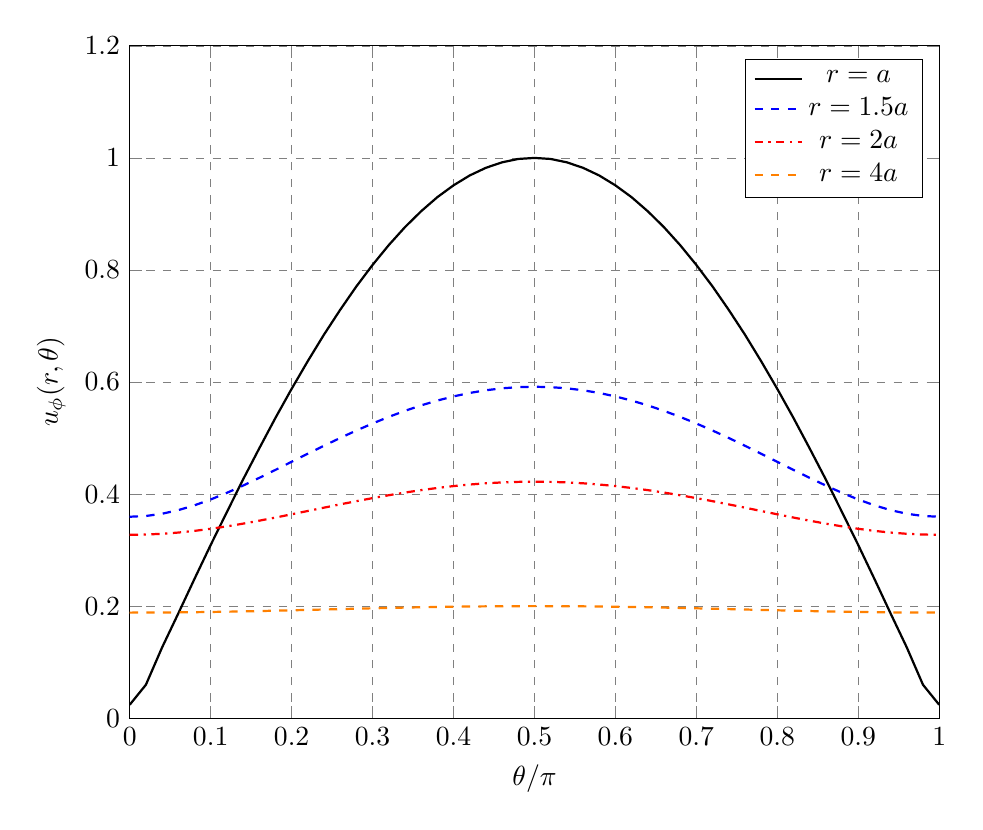
\begin{tikzpicture} \begin{axis}
[scale=1.5,
 xmin=0,  xmax=1,
 ymin=0,  ymax=1.2,
 grid=major, 
 major grid style={color=gray,line width=0.2pt, dashed},
 xlabel=$\theta / \pi$,
 ylabel={$u_\phi(r,\theta)$}
]

\addplot[line width=0.8pt, color=black] coordinates {
 ( 0.0000e+00 , 2.4102e-02 ) 
 ( 2.0000e-02 , 5.9817e-02 ) 
 ( 4.0000e-02 , 1.2641e-01 ) 
 ( 6.0000e-02 , 1.8702e-01 ) 
 ( 8.0000e-02 , 2.4868e-01 ) 
 ( 1.0000e-01 , 3.0921e-01 ) 
 ( 1.2000e-01 , 3.6786e-01 ) 
 ( 1.4000e-01 , 4.2603e-01 ) 
 ( 1.6000e-01 , 4.8156e-01 ) 
 ( 1.8000e-01 , 5.3593e-01 ) 
 ( 2.0000e-01 , 5.8777e-01 ) 
 ( 2.2000e-01 , 6.3736e-01 ) 
 ( 2.4000e-01 , 6.8465e-01 ) 
 ( 2.6000e-01 , 7.2885e-01 ) 
 ( 2.8000e-01 , 7.7061e-01 ) 
 ( 3.0000e-01 , 8.0896e-01 ) 
 ( 3.2000e-01 , 8.4433e-01 ) 
 ( 3.4000e-01 , 8.7635e-01 ) 
 ( 3.6000e-01 , 9.0476e-01 ) 
 ( 3.8000e-01 , 9.2986e-01 ) 
 ( 4.0000e-01 , 9.5099e-01 ) 
 ( 4.2000e-01 , 9.6862e-01 ) 
 ( 4.4000e-01 , 9.8229e-01 ) 
 ( 4.6000e-01 , 9.9208e-01 ) 
 ( 4.8000e-01 , 9.9809e-01 ) 
 ( 5.0000e-01 , 9.9993e-01 ) 
 ( 5.2000e-01 , 9.9809e-01 ) 
 ( 5.4000e-01 , 9.9208e-01 ) 
 ( 5.6000e-01 , 9.8229e-01 ) 
 ( 5.8000e-01 , 9.6862e-01 ) 
 ( 6.0000e-01 , 9.5099e-01 ) 
 ( 6.2000e-01 , 9.2986e-01 ) 
 ( 6.4000e-01 , 9.0476e-01 ) 
 ( 6.6000e-01 , 8.7635e-01 ) 
 ( 6.8000e-01 , 8.4433e-01 ) 
 ( 7.0000e-01 , 8.0896e-01 ) 
 ( 7.2000e-01 , 7.7061e-01 ) 
 ( 7.4000e-01 , 7.2885e-01 ) 
 ( 7.6000e-01 , 6.8465e-01 ) 
 ( 7.8000e-01 , 6.3736e-01 ) 
 ( 8.0000e-01 , 5.8777e-01 ) 
 ( 8.2000e-01 , 5.3593e-01 ) 
 ( 8.4000e-01 , 4.8156e-01 ) 
 ( 8.6000e-01 , 4.2603e-01 ) 
 ( 8.8000e-01 , 3.6786e-01 ) 
 ( 9.0000e-01 , 3.0921e-01 ) 
 ( 9.2000e-01 , 2.4868e-01 ) 
 ( 9.4000e-01 , 1.8702e-01 ) 
 ( 9.6000e-01 , 1.2641e-01 ) 
 ( 9.8000e-01 , 5.9817e-02 ) 
 ( 1.0000e+00 , 2.4102e-02 ) 
};
\addlegendentry{$r = a$};

\addplot[line width=0.8pt, color=blue, dashed] coordinates {
 ( 0.0000e+00 , 3.5964e-01 ) 
 ( 2.0000e-02 , 3.6099e-01 ) 
 ( 4.0000e-02 , 3.6499e-01 ) 
 ( 6.0000e-02 , 3.7144e-01 ) 
 ( 8.0000e-02 , 3.8003e-01 ) 
 ( 1.0000e-01 , 3.9043e-01 ) 
 ( 1.2000e-01 , 4.0228e-01 ) 
 ( 1.4000e-01 , 4.1523e-01 ) 
 ( 1.6000e-01 , 4.2897e-01 ) 
 ( 1.8000e-01 , 4.4321e-01 ) 
 ( 2.0000e-01 , 4.5767e-01 ) 
 ( 2.2000e-01 , 4.7212e-01 ) 
 ( 2.4000e-01 , 4.8637e-01 ) 
 ( 2.6000e-01 , 5.0021e-01 ) 
 ( 2.8000e-01 , 5.1350e-01 ) 
 ( 3.0000e-01 , 5.2607e-01 ) 
 ( 3.2000e-01 , 5.3781e-01 ) 
 ( 3.4000e-01 , 5.4861e-01 ) 
 ( 3.6000e-01 , 5.5835e-01 ) 
 ( 3.8000e-01 , 5.6697e-01 ) 
 ( 4.0000e-01 , 5.7437e-01 ) 
 ( 4.2000e-01 , 5.8052e-01 ) 
 ( 4.4000e-01 , 5.8534e-01 ) 
 ( 4.6000e-01 , 5.8882e-01 ) 
 ( 4.8000e-01 , 5.9092e-01 ) 
 ( 5.0000e-01 , 5.9162e-01 ) 
 ( 5.2000e-01 , 5.9092e-01 ) 
 ( 5.4000e-01 , 5.8882e-01 ) 
 ( 5.6000e-01 , 5.8534e-01 ) 
 ( 5.8000e-01 , 5.8052e-01 ) 
 ( 6.0000e-01 , 5.7437e-01 ) 
 ( 6.2000e-01 , 5.6697e-01 ) 
 ( 6.4000e-01 , 5.5835e-01 ) 
 ( 6.6000e-01 , 5.4861e-01 ) 
 ( 6.8000e-01 , 5.3781e-01 ) 
 ( 7.0000e-01 , 5.2607e-01 ) 
 ( 7.2000e-01 , 5.1350e-01 ) 
 ( 7.4000e-01 , 5.0021e-01 ) 
 ( 7.6000e-01 , 4.8637e-01 ) 
 ( 7.8000e-01 , 4.7212e-01 ) 
 ( 8.0000e-01 , 4.5767e-01 ) 
 ( 8.2000e-01 , 4.4321e-01 ) 
 ( 8.4000e-01 , 4.2897e-01 ) 
 ( 8.6000e-01 , 4.1523e-01 ) 
 ( 8.8000e-01 , 4.0228e-01 ) 
 ( 9.0000e-01 , 3.9043e-01 ) 
 ( 9.2000e-01 , 3.8003e-01 ) 
 ( 9.4000e-01 , 3.7144e-01 ) 
 ( 9.6000e-01 , 3.6499e-01 ) 
 ( 9.8000e-01 , 3.6099e-01 ) 
 ( 1.0000e+00 , 3.5964e-01 ) 
};
\addlegendentry{$r = 1.5a$};

\addplot[line width=0.8pt, color=red, dash dot] coordinates {
 ( 0.0000e+00 , 3.2743e-01 ) 
 ( 2.0000e-02 , 3.2788e-01 ) 
 ( 4.0000e-02 , 3.2923e-01 ) 
 ( 6.0000e-02 , 3.3142e-01 ) 
 ( 8.0000e-02 , 3.3441e-01 ) 
 ( 1.0000e-01 , 3.3812e-01 ) 
 ( 1.2000e-01 , 3.4245e-01 ) 
 ( 1.4000e-01 , 3.4731e-01 ) 
 ( 1.6000e-01 , 3.5260e-01 ) 
 ( 1.8000e-01 , 3.5819e-01 ) 
 ( 2.0000e-01 , 3.6400e-01 ) 
 ( 2.2000e-01 , 3.6992e-01 ) 
 ( 2.4000e-01 , 3.7586e-01 ) 
 ( 2.6000e-01 , 3.8172e-01 ) 
 ( 2.8000e-01 , 3.8741e-01 ) 
 ( 3.0000e-01 , 3.9287e-01 ) 
 ( 3.2000e-01 , 3.9802e-01 ) 
 ( 3.4000e-01 , 4.0279e-01 ) 
 ( 3.6000e-01 , 4.0714e-01 ) 
 ( 3.8000e-01 , 4.1100e-01 ) 
 ( 4.0000e-01 , 4.1435e-01 ) 
 ( 4.2000e-01 , 4.1713e-01 ) 
 ( 4.4000e-01 , 4.1933e-01 ) 
 ( 4.6000e-01 , 4.2091e-01 ) 
 ( 4.8000e-01 , 4.2187e-01 ) 
 ( 5.0000e-01 , 4.2219e-01 ) 
 ( 5.2000e-01 , 4.2187e-01 ) 
 ( 5.4000e-01 , 4.2091e-01 ) 
 ( 5.6000e-01 , 4.1933e-01 ) 
 ( 5.8000e-01 , 4.1713e-01 ) 
 ( 6.0000e-01 , 4.1435e-01 ) 
 ( 6.2000e-01 , 4.1100e-01 ) 
 ( 6.4000e-01 , 4.0714e-01 ) 
 ( 6.6000e-01 , 4.0279e-01 ) 
 ( 6.8000e-01 , 3.9802e-01 ) 
 ( 7.0000e-01 , 3.9287e-01 ) 
 ( 7.2000e-01 , 3.8741e-01 ) 
 ( 7.4000e-01 , 3.8172e-01 ) 
 ( 7.6000e-01 , 3.7586e-01 ) 
 ( 7.8000e-01 , 3.6992e-01 ) 
 ( 8.0000e-01 , 3.6400e-01 ) 
 ( 8.2000e-01 , 3.5819e-01 ) 
 ( 8.4000e-01 , 3.5260e-01 ) 
 ( 8.6000e-01 , 3.4731e-01 ) 
 ( 8.8000e-01 , 3.4245e-01 ) 
 ( 9.0000e-01 , 3.3812e-01 ) 
 ( 9.2000e-01 , 3.3441e-01 ) 
 ( 9.4000e-01 , 3.3142e-01 ) 
 ( 9.6000e-01 , 3.2923e-01 ) 
 ( 9.8000e-01 , 3.2788e-01 ) 
 ( 1.0000e+00 , 3.2743e-01 ) 
};
\addlegendentry{$r = 2a$};

\addplot[line width=0.8pt, color=orange, dashed] coordinates {
 ( 0.0000e+00 , 1.8857e-01 ) 
 ( 2.0000e-02 , 1.8862e-01 ) 
 ( 4.0000e-02 , 1.8876e-01 ) 
 ( 6.0000e-02 , 1.8899e-01 ) 
 ( 8.0000e-02 , 1.8931e-01 ) 
 ( 1.0000e-01 , 1.8972e-01 ) 
 ( 1.2000e-01 , 1.9020e-01 ) 
 ( 1.4000e-01 , 1.9074e-01 ) 
 ( 1.6000e-01 , 1.9134e-01 ) 
 ( 1.8000e-01 , 1.9199e-01 ) 
 ( 2.0000e-01 , 1.9268e-01 ) 
 ( 2.2000e-01 , 1.9339e-01 ) 
 ( 2.4000e-01 , 1.9411e-01 ) 
 ( 2.6000e-01 , 1.9484e-01 ) 
 ( 2.8000e-01 , 1.9556e-01 ) 
 ( 3.0000e-01 , 1.9625e-01 ) 
 ( 3.2000e-01 , 1.9692e-01 ) 
 ( 3.4000e-01 , 1.9754e-01 ) 
 ( 3.6000e-01 , 1.9812e-01 ) 
 ( 3.8000e-01 , 1.9863e-01 ) 
 ( 4.0000e-01 , 1.9908e-01 ) 
 ( 4.2000e-01 , 1.9946e-01 ) 
 ( 4.4000e-01 , 1.9975e-01 ) 
 ( 4.6000e-01 , 1.9997e-01 ) 
 ( 4.8000e-01 , 2.0010e-01 ) 
 ( 5.0000e-01 , 2.0014e-01 ) 
 ( 5.2000e-01 , 2.0010e-01 ) 
 ( 5.4000e-01 , 1.9997e-01 ) 
 ( 5.6000e-01 , 1.9975e-01 ) 
 ( 5.8000e-01 , 1.9946e-01 ) 
 ( 6.0000e-01 , 1.9908e-01 ) 
 ( 6.2000e-01 , 1.9863e-01 ) 
 ( 6.4000e-01 , 1.9812e-01 ) 
 ( 6.6000e-01 , 1.9754e-01 ) 
 ( 6.8000e-01 , 1.9692e-01 ) 
 ( 7.0000e-01 , 1.9625e-01 ) 
 ( 7.2000e-01 , 1.9556e-01 ) 
 ( 7.4000e-01 , 1.9484e-01 ) 
 ( 7.6000e-01 , 1.9411e-01 ) 
 ( 7.8000e-01 , 1.9339e-01 ) 
 ( 8.0000e-01 , 1.9268e-01 ) 
 ( 8.2000e-01 , 1.9199e-01 ) 
 ( 8.4000e-01 , 1.9134e-01 ) 
 ( 8.6000e-01 , 1.9074e-01 ) 
 ( 8.8000e-01 , 1.9020e-01 ) 
 ( 9.0000e-01 , 1.8972e-01 ) 
 ( 9.2000e-01 , 1.8931e-01 ) 
 ( 9.4000e-01 , 1.8899e-01 ) 
 ( 9.6000e-01 , 1.8876e-01 ) 
 ( 9.8000e-01 , 1.8862e-01 ) 
 ( 1.0000e+00 , 1.8857e-01 ) 
};
\addlegendentry{$r = 4a$};

\end{axis}
\end{tikzpicture}

\caption{Plot of the polar angle dependence (units of $\theta / \pi$ to scale from 0 to 1) of the azimuthal fluid velocity for various radial coordinates.}
\label{Fig:pde_sphericalFluidFlow_polarDependence}
\end{center}
\end{figure}

To illustrate, we consider a problem with $a = 1$ and $\omega = 1$. Figure~\ref{Fig:pde_sphericalFluidFlow_polarDependence} shows the polar angle dependence of the azimuthal velocity $u_\phi(r,\theta)$ at various radial coordinates away from the sphere. A total of 20 terms were used to generate the results. At the surface of the sphere, we see a sinusoidal dependence upon the fluid velocity with maximal flow at the equator and zero at the poles. As we move further away, the diffusive process causes the momentum to mix and the fluid velocity rises near the poles and decreases near the equator with an overall decreasing fluid velocity the further away from the sphere. As we move further away from the surface of the sphere, the curve flattens out, as the viscous shear forces dissipate any of the gradients in the polar angle such that by $r = 4a$, there is little polar dependence remaining.


%%%%%%%%%%%%%%%%%%%%%%%%%%%%%%%%%%%%%%%%%%%%%%%%%%%%%%%%%%%%%%%%%%%%%%%%%%%%%%%%%%%%%%%%%%%%%%%
%%%%%%%%%%%%%%%%%%%%%%%%%%%%%%%%%%%%%%%%%%%%%%%%%%%%%%%%%%%%%%%%%%%%%%%%%%%%%%%%%%%%%%%%%%%%%%%
\section{Finite Difference Schemes for PDEs}

While the analytical techniques often provide physical insight into the problem, rarely are they adequate for practical engineering problems. Therefore, we must resort to applying numerical schemes. A plethora of numerical methods for solving PDEs have been and continue to be developed. This section covers the standard methods.

%%%%%%%%%%%%%%%%%%%%%%%%%%%%%%%%%%%%%%%%%%%%%%%%%%%%%%%%%%%%%%%%%%%%%%%%%%%%%%%%%%%%%%%%%%%%%%%%
\subsection{Crank-Nicholson for 1-D Heat Equation}

The 1-D heat equation with a reaction coefficient can be written in the following form:
\begin{align}
  \rho(x) \dho{\phi}{t} + \dho{J}{x} + \lambda(x) \phi(x,t) = Q(x,t) .
\end{align}
Here the coefficient $\rho$ can be interpreted as a type of inertia such that the larger the value, the slower the time variation of the quantity $\phi(x,t)$; $J$ is the local flow rate given by the gradient,
\begin{align}
  J(x,t) = -D \dho{\phi}{x} ,
\end{align}
where $D$ is a diffusion coefficient; $\lambda$ is a reaction coefficient; and $Q$ is the internal source.

We must impose a spatial and temporal discretization upon the problem. As with ODEs, here we apply the cell-centered differencing scheme such that full integer indices $i$ correspond to cell centers and half-integer indices correspond to cell edges. The temporal discretization follows a different convention where integer values $n$ correspond to the solution at the beginning and end of the time steps. We use half-integer time indices to denote some average value for the time step. Uniform spatial properties are assumed within a cell and the properties are assumed to be constant in time.

The first step is to integrate the heat equation over a spatial cell having width $\Delta x_i = x_{i+1/2} - x_{i-1/2}$:
\begin{align}
  &\rho_i \dho{}{t} \left( \int_{x_{i-1/2}}^{x_{i+1/2}} \phi(x,t) dx \right)  + J(x_{i+1/2},t) - J(x_{i-1/2},t) \nonumber \\*
  &+ \lambda \int_{x_{i-1/2}}^{x_{i+1/2}} \phi(x,t) dx = \int_{x_{i-1/2}}^{x_{i+1/2}} Q(x,t) dx .
\end{align}

We then define the cell-averaged quantity as
\begin{align}
  \phi_i(t) = \frac{1}{\Delta x_i} \int_{x_{i-1/2}}^{x_{i+1/2}} \phi(x,t) dx .
\end{align}
Inserting this definition gives
\begin{align}
  \rho_i \Delta x_i \dho{\phi_i}{t}  + J(x_{i+1/2},t) - J(x_{i-1/2},t) + \lambda_i \Delta x_i \phi_i(t) = \int_{x_{i-1/2}}^{x_{i+1/2}} Q(x,t) dx .
\end{align}

To eliminate the time derivative, integrate over the time step $\Delta t_n = t_{n+1} - t_n$:
\begin{align}
  &\rho_i \Delta x_i \left[ \phi_i(t_{n+1}) - \phi_i(t_n) \right]  + \int_{t_{n}}^{t_{n+1}} J(x_{i+1/2},t) - J(x_{i-1/2},t) + \lambda_i \Delta x_i \phi_i(t) dt  \nonumber \\ 
  &= \int_{t_{n}}^{t_{n+1}} \int_{x_{i-1/2}}^{x_{i+1/2}} Q(x,t) dx dt.
\end{align}
To clean this up, we introduce a few quantities. First, we have the cell-average value at time $t_n$ as $\phi_i^n = \phi_i(t_n)$, where $n$ is a superscript not a power. We then require average values for the quantity, flow rate, and internal source. These are
\begin{subequations}
\begin{align}
  \phi_i^{n+1/2}    &= \frac{1}{\Delta t_n} \int_{t_{n}}^{t_{n+1}} \phi(x_{i+1/2},t) dt , \\
  J_{i+1/2}^{n+1/2} &= \frac{1}{\Delta t_n} \int_{t_{n}}^{t_{n+1}}    J(x_{i+1/2},t) dt , \\
  Q_i^{n+1/2}       &= \frac{1}{\Delta x_i} \frac{1}{\Delta t_n} \int_{t_{n}}^{t_{n+1}} \int_{x_{i-1/2}}^{x_{i+1/2}}   Q(x_{i+1/2},t) dx dt .
\end{align}
\end{subequations}
Then,
\begin{align}
  \rho_i \Delta x_i \left( \phi_i^{n+1} - \phi_i^n \right)  + \Delta t_n \left[ J_{i+1/2}^{n+1/2} - J_{i-1/2}^{n+1/2} + \lambda_i \Delta x_i \phi_i^{n+1/2} \right] = Delta x_i \Delta t_n Q_i^{n+1/2}.
\end{align}

We need to relate the quantity and flow rates at the beginning and end of the time step with the average value. A second-order accurate scheme may be obtained by using improved Euler and assuming that the average values within a time step are the arithmetic mean of the values at the beginning and the end:
\begin{subequations}
\begin{align}
  \phi_i^{n+1/2}    &= \frac{1}{2} \left( \phi_i^n + \phi_i^{n+1} \right) , \\
  J_{i+1/2}^{n+1/2} &= \frac{1}{2} \left( J_i^n    + J_i^{n+1}    \right) .
\end{align}
\end{subequations}
Inserting these approximations and moving all quantities with time step $n$ (which is known information from either the initial condition or a previous calculation) to the right-hand side gives
\begin{align}
  &\rho_i \Delta x_i \phi_i^{n+1} + \frac{\Delta t_n}{2} \left[ J_{i+1/2}^{n+1} - J_{i-1/2}^{n+1} + \lambda_i \Delta x_i \phi_i^{n+1} \right] \nonumber \\*
  &= \rho_i \Delta x_i \phi_i^n -  \frac{\Delta t_n}{2} \left[ J_{i+1/2}^{n} - J_{i-1/2}^{n} + \lambda_i \Delta x_i \phi_i^{n} \right] + \Delta x_i \Delta t_n Q_i^{n+1/2}.
\end{align}
Note that the internal source $Q_i^{n+1/2}$ is assumed to be known.

The next step is to approximate the flow rates $J$ with a finite difference scheme. This process is detailed in Sec.~\ref{Sec:ode_finiteDifference_reactionDiffusion} and only the end results are quoted here. 

For an interior element (not on the boundary), the flow rate on the edge of a cell is related to the cell-average quantities of the adjoining cells by
\begin{align}
  J_{i+1/2}^n = -\widetilde{D}_{i+1/2} \left( \phi_{i+1}^n - \phi_i^n \right) ,
\end{align}
where $\widetilde{D}$ is the edge-average diffusion coefficient:
\begin{align}
  \widetilde{D}_{i+1/2} = 2 \frac{ ( D_{i} / \Delta x_{i} ) ( D_{i+1} / \Delta x_{i+1} ) }{ D_{i} / \Delta x_{i} + D_{i+1} / \Delta x_{i+1} } .
\end{align}
Inserting this relationship and arranging terms gives an equation for an interior element:
\begin{align}
  &-\frac{ \Delta t_n }{2} \widetilde{D}_{i-1/2} \phi_{i-1}^{n+1} 
  + \left[ \frac{ \Delta t_n }{2} \left( \widetilde{D}_{i-1/2} + \widetilde{D}_{i+1/2} \right) + ( \lambda_i + \rho_i ) \Delta x_i \right] \phi_i^{n+1}
  -\frac{ \Delta t_n }{2} \widetilde{D}_{i+1/2} \phi_{i+1}^{n+1} \nonumber \\*
  &= \frac{ \Delta t_n }{2} \widetilde{D}_{i-1/2} \phi_{i-1}^{n} 
  - \left[ \frac{ \Delta t_n }{2} \left( \widetilde{D}_{i-1/2} + \widetilde{D}_{i+1/2} \right) + ( \lambda_i - \rho_i ) \Delta x_i \right] \phi_i^{n}
  +\frac{ \Delta t_n }{2} \widetilde{D}_{i+1/2} \phi_{i+1}^{n} \nonumber \\*
  &+ \Delta x_i \Delta t_n Q_i^{n+1/2}.
\end{align}

The equations for the boundary elements have a slightly different form. The generic form of the Robin boundary condition is written as
\begin{align}
  \alpha \phi + \beta J = \gamma  \nonumber
\end{align}
with $\alpha$, $\beta$, and $\gamma$ being coefficients that depend on the condition type. The equations for the left $(i=1)$ and right $(i=N)$ boundary elements are
\begin{subequations}
\begin{align}
  &\left[ \frac{ \Delta t_n }{2} \left( \widetilde{D}_{1/2} \alpha_\ell + \widetilde{D}_{3/2} \right) + ( \lambda_1 + \rho_1 ) \Delta x_1 \right] \phi_1^{n+1}
  -\frac{ \Delta t_n }{2} \widetilde{D}_{3/2} \phi_{2}^{n+1} \nonumber \\*
  &= - \left[ \frac{ \Delta t_n }{2} \left( \widetilde{D}_{1/2} \alpha_\ell + \widetilde{D}_{3/2} \right) + ( \lambda_1 - \rho_1 ) \Delta x_1 \right] \phi_1^{n}
  +\frac{ \Delta t_n }{2} \widetilde{D}_{3/2} \phi_{2}^{n} \nonumber \\*
  &+ \Delta x_1 \Delta t_n Q_1^{n+1/2} + \Delta t_n \widetilde{D}_{1/2} \gamma_\ell .
\end{align}
and
\begin{align}
  &-\frac{ \Delta t_n }{2} \widetilde{D}_{N-1/2} \phi_{N-1}^{n+1} 
  + \left[ \frac{ \Delta t_n }{2} \left( \widetilde{D}_{N-1/2} + \widetilde{D}_{N+1/2} \alpha_r \right) + ( \lambda_N + \rho_N ) \Delta x_N \right] \phi_N^{n+1} \nonumber \\*
  &= \frac{ \Delta t_n }{2} \widetilde{D}_{N-1/2} \phi_{N-1}^{n} 
  - \left[ \frac{ \Delta t_n }{2} \left( \widetilde{D}_{N-1/2} + \widetilde{D}_{N+1/2} \alpha_r \right) + ( \lambda_N - \rho_N ) \Delta x_N \right] \phi_N^{n} \nonumber \\*
  &+ \Delta x_N \Delta t_n Q_N^{n+1/2}  + \Delta t_n \widetilde{D}_{N+1/2} \gamma_r .
\end{align}
\end{subequations}
respectively, where the $\ell$ and $r$ subscripts denote left and right boundary coefficients and the respective edge-average diffusion coefficients are
\begin{subequations}
\begin{align}
  \widetilde{D}_{1/2}   &= \frac{ 2 D_1 / \Delta_1 }{ \alpha_\ell + \beta_\ell ( 2 D_1 / \Delta_1 ) } , \\
  \widetilde{D}_{N+1/2} &= \frac{ 2 D_{N} / \Delta_{N} }{ \alpha_r - \beta_r ( 2 D_{N} / \Delta_{N} ) } .
\end{align}
\end{subequations}

All terms on the right-hand sides of the difference equations are known either from the internal source, boundary condition, and the initial condition or previous time-step calculation. Inspecting the left-hand side, we observe that the coupling is only to the adjacent elements, meaning this system of equations can be formulated as a tridiagonal system. We have for the subdiagonal element $\ell_i$, diagonal element $d_i$, superdiagonal element $u_i$ and right-hand side element $r_i$ as follows. The left-boundary cell elements are
\begin{subequations}
\begin{align}
  d_1 &= \frac{ \Delta t_n }{2} \left( \widetilde{D}_{1/2} \alpha_\ell + \widetilde{D}_{3/2} \right) + ( \lambda_1 + \rho_1 ) \Delta x_1 , \\
  u_1 &= -\frac{ \Delta t_n }{2} \widetilde{D}_{3/2}, \\
  r_1 &= - \left[ \frac{ \Delta t_n }{2} \left( \widetilde{D}_{1/2} \alpha_\ell + \widetilde{D}_{3/2} \right) + ( \lambda_1 - \rho_1 ) \Delta x_1 \right] \phi_1^{n}
  +\frac{ \Delta t_n }{2} \widetilde{D}_{3/2} \phi_{2}^{n} \nonumber \\*
  &+ \Delta x_1 \Delta t_n Q_1^{n+1/2} + \Delta t_n \widetilde{D}_{1/2} \gamma_\ell ; 
\end{align}
the interior cell elements are
\begin{align}
  \ell_i &= -\frac{ \Delta t_n }{2} \widetilde{D}_{i-1/2}, \\
  d_i &= \frac{ \Delta t_n }{2} \left( \widetilde{D}_{i-1/2} + \widetilde{D}_{i+1/2}   \right) + ( \lambda_i + \rho_i ) \Delta x_i, \\
  u_i &= -\frac{ \Delta t_n }{2} \widetilde{D}_{i+1/2}, \\
  r_i &= \frac{ \Delta t_n }{2} \widetilde{D}_{i-1/2} \phi_{i-1}^{n} 
  - \left[ \frac{ \Delta t_n }{2} \left( \widetilde{D}_{i-1/2} + \widetilde{D}_{i+1/2} \right) + ( \lambda_i - \rho_i ) \Delta x_i \right] \phi_i^{n}
  +\frac{ \Delta t_n }{2} \widetilde{D}_{i+1/2} \phi_{i+1}^{n} \nonumber \\*
  &+ \Delta x_i \Delta t_n Q_i^{n+1/2} ,
\end{align}
for $i = 2, \ldots, N-1$. The right-boundary cell elements are
\begin{align}
  \ell_N &= -\frac{ \Delta t_n }{2} \widetilde{D}_{N-1/2}, \\
  d_N    &=  \frac{ \Delta t_n }{2} \left( \widetilde{D}_{N-1/2} + \widetilde{D}_{N+1/2} \alpha_r \right) + ( \lambda_N + \rho_N ) \Delta x_N , \\
  r_N    &= \frac{ \Delta t_n }{2} \widetilde{D}_{N-1/2} \phi_{N-1}^{n} 
  - \left[ \frac{ \Delta t_n }{2} \left( \widetilde{D}_{N-1/2} + \widetilde{D}_{N+1/2} \alpha_r \right) + ( \lambda_N - \rho_N ) \Delta x_N \right] \phi_N^{n} \nonumber \\*
  &+ \Delta x_N \Delta t_n Q_N^{n+1/2}  + \Delta t_n \widetilde{D}_{N+1/2} \gamma_r .
\end{align}
\end{subequations}

Contrasting these terms with those given for the steady-state form of the reaction-diffusion equation in Sec.~\ref{Sec:ode_finiteDifference_reactionDiffusion}, we note that the structure is the same, but there are a few notable differences. The diffusion terms have an extra factor of $\Delta t_n / 2$ that limits the amount of spreading out of the quantity within a time step. The diagonal elements contain an extra factor of $\rho \Delta x$, which arises from the time derivative. Finally, the right-hand side vector contains information about the initial condition or the field from the previous time step.

While computing the elements of the tridiagonal system is more complicated, solving for the quantity at the next time step is fundamentally the same. Performing an entire transient simulation involves repeating the tridiagonal solve for each time step.



%%%%%%%%%%%%%%%%%%%%%%%%%%%%%%%%%%%%%%%%%%%%%%%%%%%%%%%%%%%%%%%%%%%%%%%%%%%%%%%%%%%%%%%%%%%%%%%%
\subsection{Finite Difference for 2-D Reaction-Diffusion Equation}

The 2-D reaction-diffusion equation is a generalization of the Laplace equation. This has the form
\begin{align}
  -\nabla \cdot D(x,y) \nabla \phi(x,y) + \lambda(x,y) \phi(x,y) = q(x,y) .
\end{align}
Here $\phi$ is some physical quantity of interest (e.g., the neutron path-length density), $D$ is a diffusion coefficient, $\lambda$ is a reaction coefficient, and $q$ is an inhomogeneous source term. We define the flow rate vector field as
\begin{align}
  \mathbf{J}(x,y) = -D(x,y) \nabla \phi(x,y) .
\end{align}
Substituting this into the reaction-diffusion equation yields the continuity equation:
\begin{align}
  \nabla \cdot \mathbf{J}(x,y) + \lambda(x,y) \phi(x,y) = q(x,y) .
\end{align}
Expanding out the divergence in 2-D Cartesian coordinates gives
\begin{align}
  \dho{J_x}{x} + \dho{J_y}{y} + \lambda(x,y) \phi(x,y) = q(x,y) .
\end{align}
Here $J_x$ and $J_y$ are the $x$ and $y$ components of the flow rate vector $\mathbf{J}$, respectively. 

As with the 1-D case in Sec.~\ref{Sec:ode_finiteDifference_reactionDiffusion}, we define a spatial discretization. Now we apply a rectangular grid where the $(i,j)$ cell is defined such that $x_{i-1/2} \le x \le x_{i+1/2}$ and $y_{j-1/2} \le y \le y_{j+1/2}$ with spacing
\begin{subequations}
\begin{align}
  \Delta x_i &= x_{i+1/2} - x_{i-1/2}, \\
  \Delta y_j &= y_{j+1/2} - y_{j-1/2},
\end{align}
\end{subequations}
and the coordinate $(x_i,y_j)$ is taken at the center of the cell. We also demand that all reaction and diffusion coefficients are constant within each cell:
\begin{subequations}
\begin{align}
  \lambda(x,y) &= \lambda_{i,j} ,  \\
  D(x,y) &= D_{i,j},  \quad (x,y) \in (i,j).
\end{align}
\end{subequations}

We now integrate this equation over the $(i,j)$ cell and arrive at
\begin{align}
    &\int_{y_{j-1/2}}^{y_{j+1/2}} J_x(x_{i+1/2},y) - J_x(x_{i-1/2},y) dy
  +  \int_{x_{i-1/2}}^{x_{i+1/2}} J_y(x,y_{j+1/2}) - J_y(x,y_{j-1/2}) dx \nonumber \\*
  &+ \lambda_{i,j} \int_{y_{j-1/2}}^{y_{j+1/2}} \int_{x_{i-1/2}}^{x_{i+1/2}}  \phi(x,y) dx dy
  = \int_{y_{j-1/2}}^{y_{j+1/2}} \int_{x_{i-1/2}}^{x_{i+1/2}} q(x,y) dx dy .
\end{align}
We then make the following definitions for edge-averaged flow rates and cell-averaged quantities and sources:
\begin{subequations}
\begin{align}
  J_{x,{i \pm 1/2},j} &= \frac{1}{\Delta y_j} \int_{y_{j-1/2}}^{y_{j+1/2}} J_x(x_{i \pm 1/2},y) dy , \\
  J_{y,i,{j \pm 1/2}} &= \frac{1}{\Delta x_j} \int_{x_{i-1/2}}^{y_{i+1/2}} J_y(x,y_{j \pm 1/2}) dx , \\ 
  \phi_{i,j} &= \frac{1}{ \Delta x_i \Delta y_j } \int_{y_{j-1/2}}^{y_{j+1/2}} \int_{x_{i-1/2}}^{x_{i+1/2}}  \phi(x,y) dx dy , \\
  q_{i,j} &= \frac{1}{ \Delta x_i \Delta y_j } \int_{y_{j-1/2}}^{y_{j+1/2}} \int_{x_{i-1/2}}^{x_{i+1/2}}  q(x,y) dx dy .
\end{align}
\end{subequations}
We substitute in these definitions and divide by $\Delta x_i \Delta y_j$ to get
\begin{align}
    \frac{1}{\Delta x_i} \left( J_{x,{i + 1/2},j} - J_{x,{i - 1/2},j} \right)
  + \frac{1}{\Delta y_i} \left( J_{y,i,{j + 1/2}} - J_{y,i,{j - 1/2}} \right)
  + \lambda_{i,j} \phi_{i,j} = q_{i,j} .
\end{align} 

\subsubsection{Interior Cells}

As with the 1-D case, we now must apply a finite difference approximation to relate the currents to the fluxes. First we consider the case of an interior cell, i.e. one where there are neighboring cells on all four sides.

We can relate the flow rate on the left edge of the cell to the cell-average quantities in the $(i,j)$ and $(i-1,j)$ cells:
\begin{align}
  J_{x,i-1/2,j} &= -D_{i,j} \frac{ \phi_{i,j} - \phi_{i-1/2,j} }{ \Delta x_i / 2 } \\
  J_{x,i-1/2,j} &= -D_{i-1,j} \frac{ \phi_{i-1/2,j} - \phi_{i-1,j} }{ \Delta x_{i-1} / 2 } .  
\end{align}
We then equate these, solve for the quantity on the left edge $\phi_{i-1/2,j}$, and then back substitute to write the current in terms of the cell-average fluxes, eliminating the cell-edge quantity:
\begin{align}
  J_{x,i-1/2,j} &= -\widetilde{D}_{i-1/2,j} \left( \phi_{i,j} - \phi_{i-1,j} \right) ,
\end{align}
where the edge-average diffusion coefficient is
\begin{align}
  \widetilde{D}_{i-1/2,j} = 2 \frac{ ( D_{i-1,j} / \Delta x_{i-1} ) ( D_{i,j} / \Delta x_{i} ) }{ ( D_{i-1,j} / \Delta x_{i-1} )  + ( D_{i,j} / \Delta x_{i} )  } .
\end{align}
We can repeat this process for the right, bottom, and top edges to arrive at similar expressions. To illustrate, the current on the top edge is
\begin{align}
  J_{y,i,j+1/2} &= -\widetilde{D}_{i,j+1/2} \left( \phi_{i,j+1} - \phi_{i,j} \right) ,
\end{align}
with edge-average diffusion coefficient
\begin{align}
  \widetilde{D}_{i,j+1/2} = 2 \frac{ ( D_{i,j} / \Delta y_j ) ( D_{i,j+1} / \Delta y_{j+1} ) }{ ( D_{i,j} / \Delta y_{j} )  + ( D_{i,j+1} / \Delta y_{j+1} )  } .
\end{align}

We then insert these edge flow rates into the balance equation and obtain
\begin{align}
  &- \frac{\widetilde{D}_{i-1/2,j}}{\Delta x_i} \phi_{i-1,j} -  \frac{\widetilde{D}_{i,j-1/2}}{\Delta y_j} \phi_{i,j-1} \nonumber \\*
  &+ \left[ \frac{ \widetilde{D}_{i-1/2,j} + \widetilde{D}_{i+1/2,j} }{ \Delta x_i } + \frac{ \widetilde{D}_{i,j-1/2} + \widetilde{D}_{i,j+1/2} }{ \Delta y_j } + \lambda_{i,j}  \right] \phi_{i,j} \nonumber \\*
  &- \frac{\widetilde{D}_{i+1/2,j}}{\Delta x_i} \phi_{i+1,j} -  \frac{\widetilde{D}_{i,j+1/2}}{\Delta y_j} \phi_{i,j+1} = q_{i,j} . \label{Eq:pde_finiteDifference_2DDiffusionEquation}
\end{align}
Contrasting this with the 1-D result, we see that there are additional terms coupling the top and bottom edges and the coefficient on $\phi_{i,j}$ has another term.

\subsubsection{Boundary and Corner Cells}

We now need to apply a similar analysis to obtain edge-average diffusion coefficients and balance relationships at the boundaries. There are a couple additional complications in 2-D versus the 1-D case. First, the boundary conditions on each side are, in general, functions of position. For example, we write the boundary condition on the left boundary at $x = x_{1/2}$ as
\begin{align}
  \alpha(x_{1/2},y) \phi(x_{1/2},y) + \beta( x_{1/2}, y ) J(x_{1/2},y) = \gamma( x_{1/2}, y ) .
\end{align}
The coefficients $\alpha, \beta$, and $\gamma$ are now functions of $y$. To handle this in the discretization scheme, we take the boundary conditions to be spatially uniform within each each cell-edge. For the left boundary this is then
\begin{subequations}
\begin{align}
  \alpha_{1/2,j} \phi_{1/2,j} + \beta_{1/2,j} J_{1/2,j} = \gamma_{1/2,j} , \label{Eq:pde_2DdiffusionFiniteDifference_leftBC}
\end{align}
where we introduce the cell subscripts as before. On the bottom, right, and top boundaries these are
\begin{align}
  &\alpha_{i,1/2} \phi_{i,1/2} + \beta_{i,1/2} J_{i,1/2} = \gamma_{i,1/2} , \\
  &\alpha_{N_x+1/2,j} \phi_{N_x+1/2,j} + \beta_{N_x+1/2,j} J_{N_x+1/2,j} = \gamma_{N_x+1/2,j} , \\
  &\alpha_{i,N_y+1/2} \phi_{i,N_y+1/2} + \beta_{i,N_y+1/2} J_{i,N_y+1/2} = \gamma_{i,N_y+1/2} ,
\end{align}
\end{subequations}
respectively. The second complication in 2-D is that we now have to distinguish between boundary cells, where there is one boundary, and the four corner cells where there are two. This means we require special logic to handle all of the cases: one for interior cells, four for non-corner boundary cells, and another four for the corner cells.

For a cell on the left boundary, we have two equations, the finite difference approximation to the boundary,
\begin{align}
  J_{1/2,j} = -D_{1,j} \frac{ \phi_{1,j} - \phi_{1/2,j} }{ \Delta x_1 / 2 } ,
\end{align}
and Eq.~\eqref{Eq:pde_2DdiffusionFiniteDifference_leftBC} that we can solve to eliminate the edge quantity $\phi_{1/2,j}$ to solve for the flow rate at the boundary as
\begin{subequations}
\begin{align}
  J_{1/2,j} = -\widetilde{D}_{1/2,j} \left( \alpha_{1/2,j} \phi_{1,j} + \gamma_{1/2,j} \right) ,
\end{align}
where the edge-averaged left boundary diffusion coefficient is
\begin{align}
  \widetilde{D}_{1/2,j} = \frac{ 2 D_{1,j} / \Delta x_1 }{ \alpha_{1/2,j} + \beta_{1/2,j} ( 2 D_{1,j} / \Delta x_1 } .
\end{align}

The proces can be repeated for the a cell on the bottom boundary at $y = y_{1/2}$. The flow rate is
\begin{align}
  J_{i,1/2} = -\widetilde{D}_{i,1/2} \left( \alpha_{i,1/2} \phi_{i,1} + \gamma_{i,1/2} \right) ,
\end{align}
with edge-averaged diffusion coefficient of
\begin{align}
  \widetilde{D}_{i,1/2} = \frac{ 2 D_{i,1} / \Delta y_1 }{ \alpha_{i,1/2} + \beta_{i,1/2} ( 2 D_{i,1} / \Delta y_1 ) } .
\end{align}
On the right boundary, $x = x_{N_x+1/2}$, we have
\begin{align}
  J_{N_x+1/2,j} = \widetilde{D}_{N_x+1/2,j} \left( \alpha_{N_x+1/2,j} \phi_{N_x,j} - \gamma_{N_x+1/2,j} \right) ,
\end{align}
where the edge-averaged left boundary diffusion coefficient is
\begin{align}
  \widetilde{D}_{N_x+1/2,j} = \frac{ 2 D_{N_x,j} / \Delta x_{N_x} }{ \alpha_{N_x+1/2,j} - \beta_{N_x+1/2,j} ( 2 D_{N_x,j} / \Delta x_{N_x} ) } .
\end{align}
And finally on the top boundary, $y = y_{N_y+1/2}$:
\begin{align}
  J_{i,N_y+1/2} = \widetilde{D}_{i,N_y+1/2} \left( \alpha_{i,N_y+1/2} \phi_{i,N_y} - \gamma_{i,N_y+1/2} \right) ,
\end{align}
with edge-averaged diffusion coefficient of
\begin{align}
  \widetilde{D}_{i,N_y+1/2} = \frac{ 2 D_{i,N_y} / \Delta y_{N_y} }{ \alpha_{i,N_y+1/2} - \beta_{i,N_y+1/2} ( 2 D_{i,N_y} / \Delta y_{N_y} ) } .
\end{align}
\end{subequations}

Given these results for the flow rates and the associated edge-averaged diffusion coefficients on the boundaries, we can insert them into the balance equations for the cells on the boundaries and corner cells, expressing them in terms of the cell-centered quantities $\phi$. The results of these calculations are provided in Table~\ref{Table:pde_2DFiniteDifference_ReactionDiffusion_CellBalanceEquations}.


\begingroup
\renewcommand{\arraystretch}{2.2}
\begin{sidewaystable}[tb!]
\scriptsize
\caption{Cell-Balance Equations for 2-D Reaction Diffusion Equations}
\begin{center}
\begin{tabular}{|p{2cm}|l|}  \hline
%  Interior 	& $ \begin{array}{l} - \dfrac{\widetilde{D}_{i-1/2,j}}{\Delta x_i} \phi_{i-1,j} -  \dfrac{\widetilde{D}_{i,j-1/2}}{\Delta y_j} \phi_{i,j-1} \vspace{0.2cm} \\
%  + \left[ \dfrac{ \widetilde{D}_{i-1/2,j} + \widetilde{D}_{i+1/2,j} }{ \Delta x_i } + \dfrac{ \widetilde{D}_{i,j-1/2} + \widetilde{D}_{i,j+1/2} }{ \Delta y_j } + \lambda_{i,j}  \right] \phi_{i,j} \vspace{0.2cm} \\
%  - \dfrac{\widetilde{D}_{i+1/2,j}}{\Delta x_i} \phi_{i+1,j} -  \dfrac{\widetilde{D}_{i,j+1/2}}{\Delta y_j} \phi_{i,j+1} = q_{i,j} \\ \end{array} $  \\ \hline
  Interior & $- \frac{\widetilde{D}_{i-1/2,j}}{\Delta x_i} \phi_{i-1,j} -  \frac{\widetilde{D}_{i,j-1/2}}{\Delta y_j} \phi_{i,j-1} 
  + \left[ \frac{ \widetilde{D}_{i-1/2,j} + \widetilde{D}_{i+1/2,j} }{ \Delta x_i } + \frac{ \widetilde{D}_{i,j-1/2} + \widetilde{D}_{i,j+1/2} }{ \Delta y_j } + \lambda_{i,j}  \right] \phi_{i,j} 
  - \frac{\widetilde{D}_{i+1/2,j}}{\Delta x_i} \phi_{i+1,j} -  \frac{\widetilde{D}_{i,j+1/2}}{\Delta y_j} \phi_{i,j+1} = q_{i,j} $  \\ \hline
%%%%%
  Left 		& $ -  \frac{\widetilde{D}_{1,j-1/2}}{\Delta y_j} \phi_{1,j-1} + \left[ \frac{ \widetilde{D}_{1/2,j} \alpha_{1/2,j} + \widetilde{D}_{3/2,j} }{ \Delta x_1 } + \frac{ \widetilde{D}_{1,j-1/2} + \widetilde{D}_{1,j+1/2} }{ \Delta y_j } + \lambda_{1,j}  \right] \phi_{1,j} 
  - \frac{\widetilde{D}_{3/2,j}}{\Delta x_1} \phi_{2,j} -  \frac{\widetilde{D}_{1,j+1/2}}{\Delta y_j} \phi_{1,j+1} 
  = q_{1,j} + \frac{ \widetilde{D}_{1/2,j} }{ \Delta x_1 } \gamma_{1/2,j} $ \\ \hline
%%%%%
  Bottom	& $ - \frac{\widetilde{D}_{i-1/2,1}}{\Delta x_i} \phi_{i-1,1} 
  + \left[ \frac{ \widetilde{D}_{i-1/2,1} + \widetilde{D}_{i+1/2,1} }{ \Delta x_i } + \frac{ \widetilde{D}_{i,1/2} \alpha_{i,1/2} + \widetilde{D}_{i,3/2} }{ \Delta y_1 } + \lambda_{i,1}  \right] \phi_{i,1} 
  - \frac{\widetilde{D}_{i+1/2,1}}{\Delta x_i} \phi_{i+1,1} -  \frac{\widetilde{D}_{i,3/2}}{\Delta y_1} \phi_{i,2} 
  = q_{i,1} + \frac{ \widetilde{D}_{i,1/2} }{ \Delta y_1 } \gamma_{i,1/2} $ \\ \hline
%%%%%
  Right		& $ \begin{array}{l} - \frac{\widetilde{D}_{N_x-1/2,j}}{\Delta x_{N_x}} \phi_{N_x-1,j} -  \frac{\widetilde{D}_{N_x,j-1/2}}{\Delta y_j} \phi_{N_x,j-1} 
  + \left[ \frac{ \widetilde{D}_{N_x-1/2,j} + \widetilde{D}_{N_x+1/2,j} \alpha_{N_x+1/2,j} }{ \Delta x_{N_x} } + \frac{ \widetilde{D}_{N_x,j-1/2} + \widetilde{D}_{N_x,j+1/2} }{ \Delta y_j } + \lambda_{N_x,j}  \right] \phi_{N_x,j} 
  -  \frac{\widetilde{D}_{N_x,j+1/2}}{\Delta y_j} \phi_{N_x,j+1} \\
  = q_{N_x,j} + \frac{ \widetilde{D}_{N_x+1/2,j} }{ \Delta x_{N_x} } \gamma_{N_x+1/2,j} \end{array} $ \\ \hline
%%%%%
  Top		& $ \begin{array}{l} - \frac{\widetilde{D}_{i-1/2,N_y}}{\Delta x_i} \phi_{i-1,N_y} -  \frac{\widetilde{D}_{i,N_y-1/2}}{\Delta y_{N_y}} \phi_{i,N_y-1} 
  + \left[ \frac{ \widetilde{D}_{i-1/2,N_y} + \widetilde{D}_{i+1/2,N_y} }{ \Delta x_i } + \frac{ \widetilde{D}_{i,N_y-1/2} + \widetilde{D}_{i,N_y+1/2} \alpha_{i,N_y+1/2} }{ \Delta y_{N_y} } + \lambda_{i,N_y}  \right] \phi_{i,N_y} - \frac{\widetilde{D}_{i+1/2,N_y}}{\Delta x_i} \phi_{i+1,N_y}  \\
  = q_{i,N_y} +  \frac{ \widetilde{D}_{i,N_y+1/2} }{ \Delta y_{N_y} } \gamma_{i,N_y+1/2}  \end{array} $ \\ \hline  
%%%%%
  Bottom-Left & $ \begin{array}{l} \left[ \frac{ \widetilde{D}_{1/2,1} \alpha_{1/2,1} + \widetilde{D}_{3/2,1} }{ \Delta x_1 } + \frac{ \widetilde{D}_{1,1/2} \alpha_{1,1/2} + \widetilde{D}_{1,3/2} }{ \Delta y_1 } + \lambda_{1,1}  \right] \phi_{1,1} 
  - \frac{\widetilde{D}_{3/2,1}}{\Delta x_1} \phi_{2,1} -  \frac{\widetilde{D}_{1,3/2}}{\Delta y_1} \phi_{1,2} 
  = q_{1,1} + \frac{ \widetilde{D}_{1/2,1} }{ \Delta x_1 } \gamma_{1/2,1} + \frac{ \widetilde{D}_{1,1/2} }{ \Delta y_1 } \gamma_{1,1/2} \\ \end{array} $ \\ \hline
%%%%%
  Bottom-Right &  $ \begin{array}{l} - \frac{\widetilde{D}_{N_x-1/2,1}}{\Delta x_{N_x}} \phi_{N_x-1,1} 
  + \left[ \frac{ \widetilde{D}_{N_x-1/2,1} + \widetilde{D}_{N_x+1/2,1} \alpha_{N_x+1/2,1} }{ \Delta x_{N_x} } + \frac{ \widetilde{D}_{N_x,1/2} \alpha_{N_x,1/2} + \widetilde{D}_{N_x,3/2} }{ \Delta y_1 } + \lambda_{N_x,1}  \right] \phi_{N_x,1}
   -  \frac{\widetilde{D}_{N_x,3/2}}{\Delta y_1} \phi_{N_x,2} \\
  = q_{N_x,1} + \frac{ \widetilde{D}_{N_x+1/2,1} }{ \Delta x_{N_x} } \gamma_{N_x+1/2,1} + \frac{ \widetilde{D}_{N_x,1/2} }{ \Delta y_1 } \gamma_{N_x,1/2}  \\ \end{array} $ \\ \hline
%%%%%
  Top-Left & $ \begin{array}{l} -  \frac{\widetilde{D}_{1,N_y-1/2}}{\Delta y_{N_y}} \phi_{1,N_y-1} 
  + \left[ \frac{ \widetilde{D}_{1/2,N_y} \alpha_{1/2,N_y} + \widetilde{D}_{3/2,N_y} }{ \Delta x_1 } + \frac{ \widetilde{D}_{1,N_y-1/2} + \widetilde{D}_{1,N_y+1/2} \alpha_{1,N_y+1/2} }{ \Delta y_{N_y} } + \lambda_{1,N_y}  \right] \phi_{1,N_y} 
  - \frac{\widetilde{D}_{3/2,N_y}}{\Delta x_1} \phi_{2,N_y} \\
  = q_{1,N_y} + \frac{ \widetilde{D}_{1/2,N_y} }{ \Delta x_1 } \gamma_{1/2,N_y} + \frac{ \widetilde{D}_{1,N_y+1/2} }{ \Delta y_{N_y} } \gamma_{1,N_y+1/2} \\ \end{array} $ \\ \hline  
%%%%%
  Top-Right & $ \begin{array}{l} - \frac{\widetilde{D}_{N_x-1/2,N_y}}{\Delta x_{N_x}} \phi_{N_x-1,N_y} -  \frac{\widetilde{D}_{N_x,N_y-1/2}}{\Delta y_{N_y}} \phi_{N_x,N_y-1}
  + \left[ \frac{ \widetilde{D}_{N_x-1/2,N_y} + \widetilde{D}_{N_x+1/2,N_y} \alpha_{N_x+1/2,N_y} }{ \Delta x_{N_x} } + \frac{ \widetilde{D}_{N_x,N_y-1/2} + \widetilde{D}_{N_x,N_y+1/2} \alpha_{N_x,N_y+1/2} }{ \Delta y_{N_y} } 
  + \lambda_{N_x,N_y}  \right] \phi_{N_x,N_y} \\
  = q_{i,N_y} +  \frac{ \widetilde{D}_{N_x+1/2,N_y} }{ \Delta x_{N_x} } \gamma_{N_x+1/2,N_y}  +  \frac{ \widetilde{D}_{N_x,N_y+1/2} }{ \Delta y_{N_y} } \gamma_{N_x,N_y+1/2}  \\ \end{array} $ \\ \hline  
\end{tabular}
\end{center}
\label{Table:pde_2DFiniteDifference_ReactionDiffusion_CellBalanceEquations}
\end{sidewaystable}%
\endgroup
\clearpage

%Furthermore, we can express the edge-averaged diffusion coefficients in terms of the general albedo boundary condition in the same manner as for the 1-D case, but now we have four values of $\beta$ to consider for each boundary---in principle we could make these functions of $x$ or $y$ as well, but we leave including these complications as exercises.




\subsubsection{Gauss-Seidel Iteration Scheme and Successive Overrelaxation}

The linear system given by Eq.~\eqref{Eq:pde_finiteDifference_2DDiffusionEquation} for the interior cells and the associated results for the boundary and corner points do not, unlike for the 1-D case, form a tridiagonal system. Rather, it is a banded tridiagonal system. Unfortunately, the simplistic tridiagonal solver cannot be used. Instead, we employ an iterative solution scheme such as Gauss-Seidel. A couple comments. One question is whether convergence can be guaranteed. Recall that if the matrix $\mathbf{A}$ is diagonally dominant, than the algorithm will converge. We can show that for this case, diagonal dominance is guaranteed. The second point is that, as we will see, we do not actually need to represent the matrices explicitly. This is because the second-derivative operator introduces coupling only between one point and its (four) adjacent points. On account of this, the matrix is sparse and has a pattern. Therefore, we can devise a scheme that only requires representing the non-zero coefficients in vectors corresponding to their relative orientation with respect to the equation being solved.

To apply this to the 2-D neutron diffusion equation, can express Eq.~\eqref{Eq:pde_finiteDifference_2DDiffusionEquation} compactly as
\begin{align}
  C_m \phi_m + L_m \phi_{m-1} + R_m \phi_{m+1} + B_m \phi_{m-N} + A_m \phi_{m+N} = r_m, \quad m = i + jN_x.
\end{align}
Here $m$ represents a flattened one-dimensional index,
\begin{align}
  m = i + ( j - 1 ) N_x, \quad i = 1, \ldots, N_x, \quad j = 1, \ldots, N_y , \quad m = 1, \ldots N_x N_y ,
\end{align}
and the coefficients are as follows: $C_m$ on the center element or cell, which is given by the correspoinding term in square brackets in Table~\ref{Table:pde_2DFiniteDifference_ReactionDiffusion_CellBalanceEquations}. For an interior element, this is
\begin{subequations}
\begin{align}
  C_m = \frac{ \widetilde{D}_{i-1/2,j} + \widetilde{D}_{i+1/2,j} }{ \Delta x_i } + \frac{ \widetilde{D}_{i,j-1/2} + \widetilde{D}_{i,j+1/2} }{ \Delta y_j } + \lambda_{i,j} ,
\end{align}
and the boundary and corner cells follow from the table. The remaining coefficients have the same form regardless as to whether the cell is interior or not. We have: $L_m$ on the cell to the left, 
\begin{align}
  L_m = - \frac{\widetilde{D}_{i-1/2,j}}{\Delta x_i} ;
\end{align}
$R_m$ on the cell to the right, 
\begin{align}
  R_m = -\frac{\widetilde{D}_{i+1/2,j}}{\Delta x_i} ;
\end{align}
$B_m$ for the cell below, 
\begin{align}
  B_m = - \frac{\widetilde{D}_{i,j-1/2}}{\Delta y_j} ;
\end{align}
$A_m$ for the cell above, 
\begin{align}
  A_m = -  \frac{\widetilde{D}_{i,j+1/2}}{\Delta y_j} .
\end{align}
And finally, $r_m$ is the right-hand side or inhomogeneous source, which is the right-hand side of Table~\ref{Table:pde_2DFiniteDifference_ReactionDiffusion_CellBalanceEquations}. For an interior cell this is
\begin{align}
  r_m = q_{i,j},
\end{align}
\end{subequations}
and we apply the respective forms for the boundary and corner cells.

Once the equations have been written down, we then need to proceed with solving them. This can be represented as as matrix algebra $\mathbf{A x} = \mathbf{b}$ problem using the flattened index $m$. The ordering of the index is in such a manner that it gives the matrix a regular structure. This matrix can be organized into a banded-tridiagonal structure. An example of this for the grid 6$\times$5 grid is as follows:
\begin{align} \fontsize{5}{7}
  \left[ \begin{array}{	p{0.3em} p{0.3em} p{0.3em} p{0.3em} p{0.3em} p{0.8em} | 
  						p{0.3em} p{0.3em} p{0.3em} p{0.3em} p{0.3em} p{0.8em} | 
						p{0.3em} p{0.3em} p{0.3em} p{0.3em} p{0.3em} p{0.8em} |
						p{0.3em} p{0.3em} p{0.3em} p{0.3em} p{0.3em} p{0.8em} |
						p{0.3em} p{0.3em} p{0.3em} p{0.3em} p{0.3em} p{0.8em} } 
%%% 1,1 %%%
  $C_1$ & $R_1$ & $0$ 	& $0$ 	& $0$ 	& $0$ 	& 
  $A_1$ & $0$	& $0$ 	& $0$ 	& $0$ 	& $0$	& 
  $0$ 	& $0$ 	& $0$ 	& $0$ 	& $0$ 	& $0$ 	& 
  $0$ 	& $0$ 	& $0$ 	& $0$ 	& $0$ 	& $0$ 	& 
  $0$ 	& $0$ 	& $0$ 	& $0$ 	& $0$	& $0$	\vspace{-1.5em} \\ 
%%% 2,1 %%%
  $L_2$ & $C_2$ & $R_2$ & $0$ 	& $0$ 	& $0$ 	&
  $0$ 	& $A_2$	& $0$ 	& $0$ 	& $0$ 	& $0$	&
  $0$ 	& $0$ 	& $0$ 	& $0$ 	& $0$ 	& $0$ 	&
  $0$ 	& $0$ 	& $0$ 	& $0$ 	& $0$ 	& $0$ 	&
  $0$ 	& $0$ 	& $0$ 	& $0$ 	& $0$	& $0$	\vspace{-1.5em} \\ 
%%% 3,1 %%%
  $0$	& $L_3$ & $C_3$ & $R_3$ & $0$ 	& $0$ 	&
  $0$ 	& $0$ 	& $A_3$	& $0$	& $0$ 	& $0$	&
  $0$ 	& $0$ 	& $0$ 	& $0$ 	& $0$ 	& $0$ 	&
  $0$ 	& $0$ 	& $0$ 	& $0$ 	& $0$ 	& $0$ 	&
  $0$ 	& $0$ 	& $0$ 	& $0$ 	& $0$	& $0$	\vspace{-1.5em} \\ 
%%% 4,1 %%%
  $0$	& $0$	& $L_4$ & $C_4$ & $R_4$ & $0$ 	&
  $0$ 	& $0$ 	& $0$ 	& $A_4$	& $0$ 	& $0$	& 
  $0$ 	& $0$ 	& $0$ 	& $0$ 	& $0$ 	& $0$ 	& 
  $0$ 	& $0$ 	& $0$ 	& $0$ 	& $0$ 	& $0$ 	& 
  $0$ 	& $0$ 	& $0$ 	& $0$ 	& $0$	& $0$	\vspace{-1.5em} \\ 
%%% 5,1 %%%
  $0$	& $0$	& $0$	& $L_5$ & $C_5$ & $R_5$ &
  $0$ 	& $0$ 	& $0$ 	& $0$ 	& $A_5$	& $0$	&
  $0$ 	& $0$ 	& $0$ 	& $0$ 	& $0$ 	& $0$ 	&
  $0$ 	& $0$ 	& $0$ 	& $0$ 	& $0$ 	& $0$ 	&
  $0$ 	& $0$ 	& $0$ 	& $0$ 	& $0$	& $0$	\vspace{-1.5em} \\ 
%%% 6,1 %%%
  $0$	& $0$	& $0$	& $0$	& $L_6$ & $C_6$ &
  $0$ 	& $0$ 	& $0$ 	& $0$ 	& $0$	& $A_6$	&
  $0$	& $0$ 	& $0$ 	& $0$ 	& $0$ 	& $0$ 	&
  $0$ 	& $0$ 	& $0$ 	& $0$ 	& $0$ 	& $0$ 	&
  $0$ 	& $0$ 	& $0$ 	& $0$ 	& $0$	& $0$	\vspace{-1.5em} \\ \hline
%%% 1,2 %%%
  $B_7$	& $0$	& $0$	& $0$	& $0$	& $0$ 	&
  $C_7$ & $R_7$ & $0$ 	& $0$ 	& $0$	& $0$	& 
  $A_7$	& $0$	& $0$ 	& $0$ 	& $0$ 	& $0$ 	&
  $0$ 	& $0$ 	& $0$ 	& $0$ 	& $0$ 	& $0$ 	&
  $0$ 	& $0$ 	& $0$ 	& $0$ 	& $0$	& $0$	\vspace{-1.5em} \\ 
%%% 2,2 %%%
  $0$	& $B_8$	& $0$	& $0$	& $0$	& $0$	&
  $L_8$ & $C_8$ & $R_8$ & $0$ 	& $0$	& $0$	&
  $0$	& $A_8$	& $0$	& $0$ 	& $0$ 	& $0$ 	&
  $0$ 	& $0$ 	& $0$ 	& $0$ 	& $0$ 	& $0$ 	&
  $0$ 	& $0$ 	& $0$ 	& $0$ 	& $0$	& $0$	\vspace{-1.5em} \\ 
%%% 3,2 %%%
  $0$	& $0$	& $B_9$	& $0$	& $0$	& $0$	&
  $0$	& $L_9$ & $C_9$ & $R_9$ & $0$	& $0$	&
  $0$	& $0$	& $A_9$	& $0$	& $0$ 	& $0$ 	&
  $0$ 	& $0$ 	& $0$ 	& $0$ 	& $0$ 	& $0$ 	&
  $0$ 	& $0$ 	& $0$ 	& $0$ 	& $0$	& $0$	\vspace{-1.5em} \\ 
%%% 4,2 %%%
  $0$		& $0$		& $0$		& $B_{10}$	& $0$		& $0$	&
  $0$		& $0$		& $L_{10}$ 	& $C_{10}$ 	& $R_{10}$ 	& $0$	&
  $0$		& $0$		& $0$		& $A_{10}$	& $0$		& $0$ 	&
  $0$ 		& $0$ 		& $0$ 		& $0$ 		& $0$ 		& $0$ 	&
  $0$ 		& $0$ 		& $0$ 		& $0$ 		& $0$		& $0$	\vspace{-1.5em} \\ 
%%% 5,2 %%%
  $0$		& $0$		& $0$		& $0$		& $B_{11}$	& $0$		&
  $0$		& $0$		& $0$		& $L_{11}$ 	& $C_{11}$ 	& $R_{11}$ 	&
  $0$		& $0$		& $0$		& $0$		& $A_{11}$	& $0$		&
  $0$ 		& $0$ 		& $0$ 		& $0$ 		& $0$ 		& $0$ 		&
  $0$ 		& $0$ 		& $0$ 		& $0$ 		& $0$		& $0$		\vspace{-1.5em} \\ 
%%% 6,2 %%%
  $0$		& $0$		& $0$		& $0$		& $0$		& $B_{12}$	&
  $0$		& $0$		& $0$		& $0$		& $L_{12}$ 	& $C_{12}$ 	&
  $0$ 		& $0$		& $0$		& $0$		& $0$		& $A_{12}$	&
  $0$		& $0$ 		& $0$ 		& $0$ 		& $0$ 		& $0$ 		&
  $0$ 		& $0$ 		& $0$ 		& $0$ 		& $0$		& $0$		\vspace{-1.5em} \\ \hline
%%% 1,3 %%%
  $0$		& $0$		& $0$		& $0$		& $0$		& $0$		&
  $B_{13}$	& $0$		& $0$		& $0$		& $0$ 		& $0$ 		&
  $C_{13}$ 	& $R_{13}$	& $0$		& $0$		& $0$		& $0$		&
  $A_{13}$	& $0$ 		& $0$ 		& $0$ 		& $0$ 		& $0$ 		&
  $0$ 		& $0$ 		& $0$ 		& $0$ 		& $0$		& $0$		\vspace{-1.5em} \\ 
%%% 2,3 %%%
  $0$		& $0$		& $0$		& $0$		& $0$		& $0$		&
  $0$		& $B_{14}$	& $0$		& $0$		& $0$		& $0$ 		& 
  $L_{14}$	& $C_{14}$ 	& $R_{14}$	& $0$		& $0$		& $0$		& 
  $0$		& $A_{14}$	& $0$ 		& $0$ 		& $0$ 		& $0$ 		& 
  $0$ 		& $0$ 		& $0$ 		& $0$ 		& $0$		& $0$		\vspace{-1.5em} \\ 
%%% 3,3 %%%
  $0$		& $0$		& $0$		& $0$		& $0$		& $0$		&
  $0$		& $0$		& $B_{15}$	& $0$		& $0$		& $0$		& 
  $0$		& $L_{15}$	& $C_{15}$ 	& $R_{15}$	& $0$		& $0$		& 
  $0$		& $0$		& $A_{15}$	& $0$ 		& $0$ 		& $0$ 		& 
  $0$ 		& $0$ 		& $0$ 		& $0$ 		& $0$		& $0$		\vspace{-1.5em} \\ 
%%% 4,3 %%%
  $0$		& $0$		& $0$		& $0$		& $0$		& $0$		&
  $0$		& $0$		& $0$		& $B_{16}$	& $0$		& $0$		& 
  $0$		& $0$		& $L_{16}$	& $C_{16}$ 	& $R_{16}$	& $0$		& 
  $0$		& $0$		& $0$		& $A_{16}$	& $0$ 		& $0$ 		& 
  $0$ 		& $0$ 		& $0$ 		& $0$ 		& $0$		& $0$		\vspace{-1.5em} \\ 
%%% 5,3 %%%
  $0$		& $0$		& $0$		& $0$		& $0$		& $0$		&
  $0$		& $0$		& $0$		& $0$		& $B_{17}$	& $0$		&
  $0$		& $0$		& $0$		& $L_{17}$	& $C_{17}$ 	& $R_{17}$	& 
  $0$		& $0$		& $0$		& $0$		& $A_{17}$	& $0$ 		& 
  $0$ 		& $0$ 		& $0$ 		& $0$ 		& $0$		& $0$		\vspace{-1.5em} \\ 
%%% 6,3 %%%
  $0$		& $0$		& $0$		& $0$		& $0$		& $0$		&
  $0$		& $0$		& $0$		& $0$		& $0$		& $B_{18}$	& 
  $0$		& $0$		& $0$		& $0$		& $L_{18}$	& $C_{18}$ 	& 
  $0$		& $0$		& $0$		& $0$		& $0$		& $A_{18}$	& 
  $0$ 		& $0$ 		& $0$ 		& $0$ 		& $0$		& $0$		\vspace{-1.5em} \\ \hline
%%% 1,4 %%%
  $0$		& $0$		& $0$		& $0$		& $0$		& $0$		&
  $0$		& $0$		& $0$		& $0$		& $0$		& $0$		&
  $B_{19}$	& $0$		& $0$		& $0$		& $0$ 		& $0$ 		&
  $C_{19}$ 	& $R_{19}$	& $0$		& $0$		& $0$		& $0$		&
  $A_{19}$	& $0$ 		& $0$ 		& $0$ 		& $0$ 		& $0$ 		\vspace{-1.5em} \\ 
%%% 2,4 %%%
  $0$		& $0$		& $0$		& $0$		& $0$		& $0$		&
  $0$		& $0$		& $0$		& $0$		& $0$		& $0$		&
  $0$		& $B_{20}$	& $0$		& $0$		& $0$		& $0$ 		& 
  $L_{20}$	& $C_{20}$ 	& $R_{20}$	& $0$		& $0$		& $0$		& 
  $0$		& $A_{20}$	& $0$ 		& $0$ 		& $0$ 		& $0$ 		\vspace{-1.5em} \\ 
%%% 3,4 %%%
  $0$		& $0$		& $0$		& $0$		& $0$		& $0$		&
  $0$		& $0$		& $0$		& $0$		& $0$		& $0$		&
  $0$		& $0$		& $B_{21}$	& $0$		& $0$		& $0$		& 
  $0$		& $L_{21}$	& $C_{21}$ 	& $R_{21}$	& $0$		& $0$		& 
  $0$		& $0$		& $A_{21}$	& $0$ 		& $0$ 		& $0$ 		\vspace{-1.5em} \\ 
%%% 4,4 %%%
  $0$		& $0$		& $0$		& $0$		& $0$		& $0$		&
  $0$		& $0$		& $0$		& $0$		& $0$		& $0$		&
  $0$		& $0$		& $0$		& $B_{22}$	& $0$		& $0$		& 
  $0$		& $0$		& $L_{22}$	& $C_{22}$ 	& $R_{22}$	& $0$		& 
  $0$		& $0$		& $0$		& $A_{22}$	& $0$ 		& $0$ 		\vspace{-1.5em} \\ 
%%% 5,4 %%%
  $0$		& $0$		& $0$		& $0$		& $0$		& $0$		&
  $0$		& $0$		& $0$		& $0$		& $0$		& $0$		&
  $0$		& $0$		& $0$		& $0$		& $B_{23}$	& $0$		&
  $0$		& $0$		& $0$		& $L_{23}$	& $C_{23}$ 	& $R_{23}$	& 
  $0$		& $0$		& $0$		& $0$		& $A_{23}$	& $0$ 		\vspace{-1.5em} \\ 
%%% 6,4 %%%
  $0$		& $0$		& $0$		& $0$		& $0$		& $0$		&
  $0$		& $0$		& $0$		& $0$		& $0$		& $0$		&
  $0$		& $0$		& $0$		& $0$		& $0$		& $B_{24}$	& 
  $0$		& $0$		& $0$		& $0$		& $L_{24}$	& $C_{24}$ 	& 
  $0$		& $0$		& $0$		& $0$		& $0$		& $A_{24}$	\vspace{-1.5em} \\ \hline
%%% 1,5 %%%
  $0$		& $0$		& $0$		& $0$		& $0$		& $0$		&
  $0$		& $0$		& $0$		& $0$		& $0$		& $0$		&
  $0$		& $0$		& $0$		& $0$		& $0$		& $0$		&
  $B_{25}$	& $0$		& $0$		& $0$		& $0$ 		& $0$ 		&
  $C_{25}$ 	& $R_{25}$	& $0$		& $0$		& $0$		& $0$		\vspace{-1.5em} \\ 
%%% 2,5 %%%
  $0$		& $0$		& $0$		& $0$		& $0$		& $0$		&
  $0$		& $0$		& $0$		& $0$		& $0$		& $0$		&
  $0$		& $0$		& $0$		& $0$		& $0$		& $0$		&
  $0$		& $B_{26}$	& $0$		& $0$		& $0$		& $0$ 		& 
  $L_{26}$	& $C_{26}$ 	& $R_{26}$	& $0$		& $0$		& $0$		\vspace{-1.5em} \\ 
%%% 3,5 %%%
  $0$		& $0$		& $0$		& $0$		& $0$		& $0$		&
  $0$		& $0$		& $0$		& $0$		& $0$		& $0$		&
  $0$		& $0$		& $0$		& $0$		& $0$		& $0$		&
  $0$		& $0$		& $B_{27}$	& $0$		& $0$		& $0$		& 
  $0$		& $L_{27}$	& $C_{27}$ 	& $R_{27}$	& $0$		& $0$		\vspace{-1.5em} \\ 
%%% 4,5 %%%
  $0$		& $0$		& $0$		& $0$		& $0$		& $0$		&
  $0$		& $0$		& $0$		& $0$		& $0$		& $0$		&
  $0$		& $0$		& $0$		& $0$		& $0$		& $0$		&
  $0$		& $0$		& $0$		& $B_{28}$	& $0$		& $0$		& 
  $0$		& $0$		& $L_{28}$	& $C_{28}$ 	& $R_{28}$	& $0$		\vspace{-1.5em} \\ 
%%% 5,5 %%%
  $0$		& $0$		& $0$		& $0$		& $0$		& $0$		&
  $0$		& $0$		& $0$		& $0$		& $0$		& $0$		&
  $0$		& $0$		& $0$		& $0$		& $0$		& $0$		&
  $0$		& $0$		& $0$		& $0$		& $B_{29}$	& $0$		&
  $0$		& $0$		& $0$		& $L_{29}$	& $C_{29}$ 	& $R_{29}$	\vspace{-1.5em} \\ 
%%% 6,5 %%%
  $0$		& $0$		& $0$		& $0$		& $0$		& $0$		&
  $0$		& $0$		& $0$		& $0$		& $0$		& $0$		&
  $0$		& $0$		& $0$		& $0$		& $0$		& $0$		&
  $0$		& $0$		& $0$		& $0$		& $0$		& $B_{30}$	& 
  $0$		& $0$		& $0$		& $0$		& $L_{30}$	& $C_{30}$ 	\vspace{-1.5em} \\ 
\end{array} \right] . \nonumber
\end{align}
Partitions are included in this matrix to illustrate where the problem edges reside and to highlight features in the matrix structure. First, it should be apparent that most elements in this matrix are zero, i.e., the matrix is sparse. Therefore, we do not need to explicitly represent it on the computer (which can be prohibitive as the size of the grid becomes large). 

Starting the lower-left corner $m = 1$ or $\phi_{1,1}$, we solve for the corresponding value of the field there. For the corner point, the value can be solved as
\begin{align}
  \phi_1^{(n+1)} = \frac{1}{C_1} \left( r_1 - R_1 \phi_2^{(n)} - A_1 \phi_{1+N_x}^{(n)} \right) .
\end{align}
Here we introduced a superscript in parentheses to denote an iteration index and use the flattened index. Next, we move to the right and solve for the adjacent value $\phi_2 = \phi_{2,0}$, using the new value of $\phi_{1,1}$ we just solved for:
\begin{align}
  \phi_2^{(n+1)} = \frac{1}{C_2} \left( r_2 - L_2 \phi_1^{(n+1)} - R_2 \phi_3^{(n)} - A_2 \phi_{2+N_x}^{(n)} \right) .
\end{align}
Again, the iteration index of $(n+1)$ on $\phi_1$ is because we are using the value we just computed. We then continue the process, moving to the right until we reach the end of the first row. For a generic element on this row with flattened index $m = i$, we have
\begin{align}
  \phi_{i}^{(n+1)} = \frac{1}{C_i} \left( r_i - L_i \phi_{i-1}^{(n+1)} - R_i \phi_{i+1}^{(n)} - A_i \phi_{i+N_x}^{(n)} \right) ,
\end{align}
and at the lower-right corner we have
\begin{align}
  \phi_{N_x}^{(n+1)} = \frac{1}{C_{N_x}} \left( r_{N_x} - L_{N_x} \phi_{N_x-1}^{(n+1)} - A_{N_x} \phi_{2N_x}^{(n)} \right) .
\end{align}

Next, we move onto the second row and solve for each field value from left to right and then over the rows from bottom to top, always using the most up-to-date information. For a generic interior element, we have
\begin{align}
  \phi_m^{(n+1)} = \frac{1}{C_m} \left( r_m - L_m \phi_{m-1}^{(n+1)} - B_m \phi_{m-N_x}^{(n+1)} - R_{m} \phi_{m+1}^{(n)} - A_{m} \phi_{m+N_x}^{(n)} \right) .
\end{align}
Note that the element to the left and below have already been solved for on this iteration, so we use those values in the equation.

After we solve for the element at the top-right corner $\phi_{N_x N_y} = \phi_{N_x,N_y}$, we check whether the new field values are within some tolerance $\epsilon$ of the previous solution. This is done using the following norm:
\begin{align}
  \dfrac{ \sum_{m=1}^{N_x N_y}  | \phi_{m}^{(n+1)} - \phi_{m}^{(n)} | }{ \sum_{m=1}^{N_x N_y}  | \phi_{m}^{(n+1)} | }  < \epsilon .
\end{align} 
If the tolerance is satisfied, the calculation finishes and the current solution is output. If it is not, the process is repeated for more iterations until convergence is achieved.

The implementation of this is actually (perhaps surprisingly) not too difficult. The coefficient vectors $C, L, R, B, A$ along with the inhomogeneous right-hand side source term can be precomputed. We then begin with the top row of the matrix and solve for a new value using the appropriate equation, computing the contribution to the error, and then overwriting the old value with that new value. Next, we proceed down the rows, repeating the process and using the most up-to-date information. The tricky part is handling the edges gracefully so as not to access invalid array elements. These can be handled either with if-then statements or by sizing vectors larger than they need to be and storing zeroes in those elements.

The convergence rate for Gauss-Seidel can be slow for large linear systems. Accelerating this convergence becomes especially important because we can have multiple energy groups (typically not too many for diffusion, thankfully) and, more significantly, an outer iteration loop to converge the fission source. The most common acceleration method is called \emph{successive over-relaxation}, which is a kind of extrapolation.

We introduce an over-relaxation parameter $\omega$ that is typically on the domain $1 \le \omega < 2$. The value of $\omega = 1$ reduces to Gauss-Seidel and $\omega \ge 2$ can be numerically unstable. Note that sometimes we let $\omega < 1$ to under-relax numerical schemes to assist with numerical stability. 

Anyway, we return to the $\mathbf{Ax} = \mathbf{b}$ problem. We split out the matrix $\mathbf{A}$ as before and then multiply by a factor $\omega$. Moving the upper triangular part to the right-hand side we get
\begin{align}
   \left( \omega \mathbf{L} + \omega  \mathbf{D} \right) \mathbf{x} = \omega \mathbf{b} - \omega \mathbf{U x }
\end{align}
Next we add $( 1 - \omega ) \mathbf{D x}$ to both sides of the equation. After using the fact that $\omega + ( 1 - \omega ) = 1$ and applying iteration indices we have
\begin{align}
   \left[ \omega \mathbf{L} + \mathbf{D} \right] \mathbf{x}^{(n+1)} = \omega  \mathbf{b} + \left[ ( 1 - \omega ) \mathbf{D} - \omega \mathbf{U} \right] \mathbf{ x }^{(n)} .
\end{align}

We can then do as before and write out each term given that the system only couples with its adjacent grid points. To illustrate, the updated flux for the generic interior grid point is
\begin{align}
  \phi_m^{(n+1)} = ( 1 - \omega ) \phi_m^{(n)} +  \frac{\omega}{C_m} \left( r_m - L_m \phi_{m-1}^{(n+1)} - B_m \phi_{m-N_x}^{(n+1)} - R_{m} \phi_{m+1}^{(n)} - A_{m} \phi_{m+N_x}^{(n)} \right) .
\end{align}
The other expression follow directly. By quick observation, the application of successive over-relaxation requires only a trivial modification to the equations used in the loops. This is a major reason why it is such popular acceleration scheme.

One question is the choice of $\omega$. There is a unique, optimal value of $\omega$. While there are some analyses that can be done under simple conditions to determine this, in practice this is often chosen based on numerical experimentation for the class of problems. If $\omega$ is chosen close to the optimal value, then the number of iterations required for convergence is significantly reduced.

